%% FedFACS -- revised manuscript, Springer Nature LaTeX template (sn-jnl class).
%% Place sn-jnl.cls and sn-basic.bst from the official Springer Nature template next to this file
%% (Overleaf: "Springer Nature LaTeX Template") and compile with pdfLaTeX + BibTeX.

\documentclass[pdflatex,sn-basic]{sn-jnl}

\usepackage{graphicx}
\usepackage{multirow}
\usepackage{amsmath,amssymb,amsfonts}
\usepackage{mathrsfs}
\usepackage[title]{appendix}
\usepackage{xcolor}
\usepackage{textcomp}
\usepackage{booktabs}
\usepackage{array}
\usepackage{algorithm}
\usepackage{algpseudocode}

\newcommand{\KL}{\Delta\mathrm{KL}}
\newcommand{\Fit}{\mathrm{Fitness}}
\newcommand{\todo}[1]{\textcolor{red}{[#1]}}

\begin{document}

\title[FedFACS: Fair Adaptive Client Selection]{FedFACS: A Fair Adaptive Client Selection Framework for Communication-Efficient Federated Learning}

\author*[1]{\fnm{First} \sur{Author}}\email{\todo{email}}
\author[1]{\fnm{Second} \sur{Author}}\email{\todo{email}}

\affil*[1]{\orgdiv{\todo{Department}}, \orgname{\todo{Institution}}, \orgaddress{\city{\todo{City}}, \country{\todo{Country}}}}

\abstract{Client selection in federated learning (FL) must balance predictive performance, fair participation and communication cost when client data are heterogeneous. We present FedFACS, a selection framework that ranks clients with a fitness score combining (i) the Kullback--Leibler (KL) divergence between a client's post-training predictions and those of the received global model, (ii) an idle-round fairness term and (iii) a penalty on the variability of that divergence across scoring batches. A feedback controller adapts the utility--fairness mixing coefficient from the global validation-loss trajectory, the cohort size is adapted within fixed bounds, and selected updates are aggregated with normalised, nonnegative stability weights. All candidate clients download the model, train and report a score; FedFACS reduces model-update uploads and aggregation contributions, not downloads or local computation. We evaluate it on MNIST, FMNIST, CIFAR-10 and COVID-19 Radiography under Dirichlet, two-class and noisy partitions. In single-run experiments, FedFACS reaches the target accuracy in fewer rounds than Zhai et al.\ in all nine Configuration~A settings, although DivFL is faster on MNIST; it improves accuracy over AHIBCS by 1.2, 1.2 and 0.5 points on FMNIST, CIFAR-10 and COVID-19 and lowers cumulative uploads by 1.5--4.8\%, but needs more rounds on FMNIST and CIFAR-10 and has lower COVID-19 recall (0.934 vs 0.948); and it attains a higher Jain fairness index than FairFedCS in five of six noisy-data settings. The original implementation is no longer available, so results are single-run and were not re-obtained with the corrected formulation; we state the consequences explicitly.}

\keywords{Federated learning, Client selection, Fairness, Communication efficiency, Non-IID data}

\maketitle

%% ------------------------------------------------------------------
\section{Introduction}\label{sec1}

Federated learning (FL) coordinates many devices through a central server to train a shared model while each participant keeps its data in its own environment. This makes FL attractive where data confidentiality matters, for example in smart transportation, financial services and healthcare \citep{shanmugarasa2023}. In conventional FL, training proceeds in communication rounds: the server sends the latest global model to the participating clients, which train locally and return updates for aggregation, until a performance criterion is met \citep{kairouz2021} (Fig.~\ref{fig:fl}). The repeated exchange of model parameters between clients and server is a major source of communication overhead, and it grows with the number of participants.

Training becomes harder when clients differ in data distribution, dataset size, data quality or computational capability. Such heterogeneity can create fairness problems, slow global convergence and degrade the global model \citep{kairouz2021,khajehali2023,mayhoub2024,fu2023,wen2023}. Client selection is therefore used to decide which participants contribute in each round, aiming to limit communication \citep{asad2023}, accelerate convergence and improve accuracy. Many selection techniques rely on predefined participation ratios or fixed cohort sizes \citep{lai2021,larsson2021}, while others are resource-based \citep{nishio2019,li2022}, bandwidth-based \citep{ji2023} or correlation-based \citep{cho2022,tang2021}. Most do not balance global and local factors or treat fair participation under non-IID data explicitly, so participants with larger datasets, better data or stronger resources may be selected repeatedly while others stay idle, which can bias the global model \citep{vucinich2023,ayeelyan2025}. Balancing predictive performance and fairness in client selection under non-IID data therefore remains open.

\begin{figure}[t]
\centering
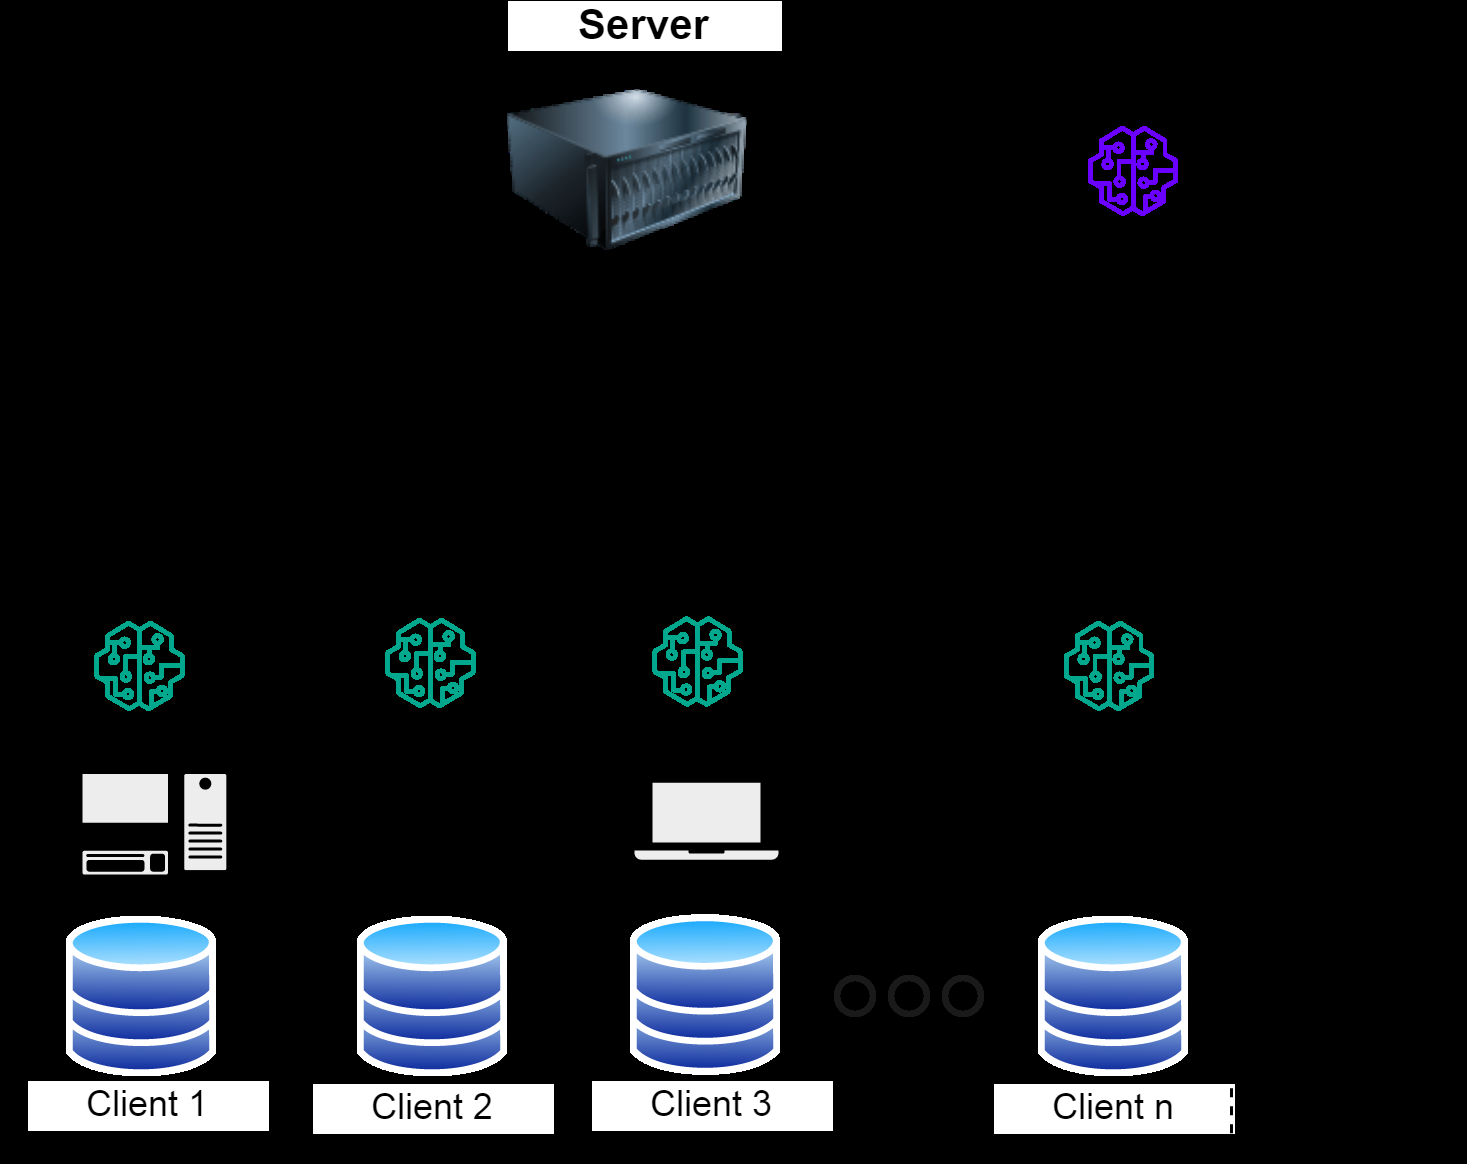
\includegraphics[width=0.62\textwidth]{figs/fig1.png}
\caption{Federated learning iterative process.}\label{fig:fl}
\end{figure}

We propose FedFACS (Federated Fair Adaptive Client Selection). FedFACS ranks clients with a fitness score built from three quantities: a utility term, a fairness term and an uncertainty penalty. The utility term is the KL divergence between a client's post-training predictive distribution and that of the received global model; it measures how far the local model has moved from the global model on the client's data. The uncertainty penalty is the variance of this divergence across scoring mini-batches. The fairness term grows with the number of consecutive rounds a client has not been selected, relative to the population mean \citep{shi2024,xu2024}. A bounded feedback rule, motivated by Lyapunov-style control \citep{chaudhari2002} but not a Lyapunov analysis, adjusts the utility--fairness mixing from the global validation-loss trajectory. The cohort size is adapted within configured integer bounds, and selected updates are combined with normalised, nonnegative stability weights.

The contributions of this work are as follows.
\begin{enumerate}
\item \textbf{A fitness score for fair adaptive selection.} We combine a KL-divergence utility, an idle-round fairness term and a batch-variance penalty into one ranking score, and state precisely what each term measures and does not measure.
\item \textbf{Convergence-aware mixing and cohort sizing.} A bounded feedback rule sets the utility--fairness coefficient, and an integer cohort rule sets the number of aggregated clients from the previous round's validation-loss reduction. Both use only information from completed FedFACS rounds. They are heuristics; no convergence or fairness guarantee is claimed.
\item \textbf{Normalised stability-weighted aggregation.} Aggregation weights are nonnegative and sum to one, with a sample-count fallback when no client has a positive stability score.
\item \textbf{An empirical study with explicit accounting.} We evaluate on four datasets under several heterogeneity settings, report where FedFACS is and is not better than the compared methods, distinguish uploads from downloads and local computation, and state the limitations of the evidence (Sections~\ref{sec:scope} and~\ref{sec:limits}).
\end{enumerate}

The rest of the paper is organised as follows. Section~\ref{sec2} reviews related work, Section~\ref{sec3} formulates the problem, Section~\ref{sec4} describes FedFACS, Section~\ref{sec5} reports the evaluation, Section~\ref{sec:limits} states limitations and Section~\ref{sec7} concludes.

%% ------------------------------------------------------------------
\section{Related work}\label{sec2}

\subsection{Classical federated learning}
FL has attracted attention in healthcare, edge computing, finance and computer vision \citep{ahmed2024,darzi2024,khan2024}, where data heterogeneity and communication overhead are the two main challenges. FedAvg averages updates from participating clients to build a shared model, but it degrades under non-IID data and ignores fairness \citep{mcmahan2017}. FedProx adds a proximal term to stabilise local training under heterogeneity, at additional computational cost \citep{li2020}. SCAFFOLD uses control variates to reduce client drift, but increases communication and can fail under strong heterogeneity \citep{karimireddy2020}. FedAdam uses an adaptive server-side optimiser, at higher server-side cost and without addressing fairness \citep{reddi2021}. FedNova normalises local updates before aggregation to remove objective inconsistency, but does not address the communication cost of many participants \citep{wang2020}.

\subsection{Client selection and model aggregation}
Classical FL assumes homogeneous data and resources; in practice neither holds, and transmitting updates from all clients every round is impractical. Selection methods include random, communication-based, utility-based, correlation-based and resource-based approaches \citep{ayeelyan2025}. Random selection with a fixed client count lacks adaptability and awareness of heterogeneity. \citet{li2024} use a performance-aware weight-decay mechanism that adapts the number of participants from historical performance. \citet{tsouvalas2024} reduce communication by compressing the model through dynamic clustered weighting, with possibly limited benefit under strong heterogeneity. \citet{vanthang2025} select informative clients from gradients and adapt thresholds in a fog-computing setting. Oort scores clients by training time, local loss and past selection count \citep{lai2021}. Power-of-Choice favours high-loss clients \citep{cho2022}. \citet{ye2025} rank clients by estimated contribution and alignment with the global model. \citet{zhai2024} select clients by a multi-armed-bandit quality metric that combines individual contribution and cross-client correlation, and weight aggregation by quality. DivFL selects diverse clients using gradient information \citep{balakrishnan2022}. \citet{nishio2019} select clients by data size, bandwidth and compute so that updates arrive within a deadline. AHIBCS uses current and historical client behaviour with an adaptive threshold, switching between a loss-based and a diversity-based strategy \citep{liu2025}.

Aggregation weights are classically proportional to local dataset sizes \citep{ayeelyan2025,zhai2024}. \citet{ji2019} use trainable attention scores to weight updates, and \citet{wu2021} weight updates by their directional alignment with the global optimisation direction; both add computational complexity and may suppress rare informative features from heterogeneous clients.

\subsection{Fairness-based client selection}
Fairness in FL aims to give all clients an opportunity to contribute \citep{huang2024}. Under non-IID data, over-exploiting high-contributing clients while under-exploring others yields a model biased toward the repeatedly selected clients, so adaptive fairness mechanisms are needed to balance exploitation and exploration \citep{bouzamoucha2025,mukhtiar2025a,mukhtiar2025b,zhang2022}. \citet{huang2020} select clients with a fairness constraint, though fairness is not guaranteed because selection is probabilistic. \citet{song2022} balance participation frequency and reputation. \citet{chaudhury2024} propose a veto-core approach to prevent client domination, at significant communication and computation cost. \citet{wang2023} use an entropy-based framework to trade fairness against accuracy. \citet{shi2023} propose FairFedCS, a Lyapunov-based selection whose score depends on reputation, participation frequency and Shapley value, and which lets clients redeem reputation, at computational overhead.

\subsection{Positioning of FedFACS}
The closest methods are Zhai et al.\ (adaptive selection and quality-weighted aggregation), AHIBCS (loss- and history-based adaptive selection) and FairFedCS (fairness-aware selection). FedFACS differs in the information its ranking uses: the divergence between local and global predictions on client-held scoring data, a server-recorded idle-round counter and a batch-variability penalty. It also differs in how it adapts the cohort size, from the previous round's validation-loss reduction, and how it weights aggregation, by a normalised nonnegative stability score. It requires every candidate to train and score before selection, which the compared selectors do not necessarily require; Section~\ref{sec4} and Section~\ref{sec:limits} state what this costs. This paper does not provide a controlled comparison of decision rules, information requirements and measured cost against these methods in a single framework.

%% ------------------------------------------------------------------
\section{Problem formulation}\label{sec3}

Let $\mathcal{C}=\{1,\dots,N\}$ be the client population, $D_i$ the dataset of client $i$, $n_i=|D_i|>0$ and $n=\sum_{i=1}^{N}n_i$. The sample-weighted learning objective and the local empirical loss are
\begin{equation}\label{eq:obj}
J(w)=\sum_{i=1}^{N}\frac{n_i}{n}\,f_i(w),\qquad n=\sum_{i=1}^{N}n_i,
\end{equation}
\begin{equation}\label{eq:loss}
f_i(w)=\frac{1}{n_i}\sum_{j=1}^{n_i}\ell\bigl(w;x_{ij},y_{ij}\bigr).
\end{equation}
Data heterogeneity makes local updates biased, unstable and noisy, and selecting all clients every round is impractical because of communication cost. At round $t$ the server therefore forms a cohort $C_k^t\subseteq\mathcal{C}$ of size $m_t$, given by Eq.~\eqref{eq:cohort}, by maximising the sum of fitness scores defined in Section~\ref{sec4}:
\begin{equation}\label{eq:sel}
C_k^t\in\operatorname*{arg\,max}_{\substack{A\subseteq\mathcal{C}\\|A|=m_t}}\ \sum_{i\in A}\Fit_i^t .
\end{equation}
Ties are resolved by ascending client identifier. The global model of the next round is the weighted average of the selected clients' models,
\begin{equation}\label{eq:agg}
w_{\mathrm{global}}^{t+1}=\sum_{i\in C_k^t}S_i^t\,w_i^t,
\end{equation}
with weights $S_i^t\ge 0$, $\sum_{i\in C_k^t}S_i^t=1$ defined in Eq.~\eqref{eq:S}.

FedFACS applies local optimisation to $f_i$, determines cohort membership by Eq.~\eqref{eq:sel} and determines the averaging weights by Eq.~\eqref{eq:S}. Equation~\eqref{eq:obj} is the reference population objective. It is not the criterion that the ranking rule optimises, and the stability weights replace the sample-size weights of Eq.~\eqref{eq:obj} without a proof that the resulting procedure minimises $J$. FedFACS should be read as a heuristic for choosing and weighting clients, not as an optimiser of Eq.~\eqref{eq:obj}.

%% ------------------------------------------------------------------
\section{The FedFACS framework}\label{sec4}

\subsection{Overview and protocol}\label{sec4.1}
FedFACS follows a synchronous client--server architecture (Fig.~\ref{fig:arch}). At round $t$ the server broadcasts the committed global model and round-start control state to all $N$ candidates (Step~1). Each candidate initialises its local model from the received global model, trains it and computes its fitness (Step~2), and reports the fitness together with its server-recorded idle counter (Step~3). Using feedback from completed rounds, the server computes the cohort size, ranks the candidates (Step~4) and selects $C_k^t$ (Step~5). Selected clients upload their trained parameters, raw stability scores and registered sample counts (Step~6). The server then aggregates with stability weights, validates the result and updates its control state (Step~7). Training stops when the performance criterion or the round budget is reached.

\emph{All $N$ candidates therefore incur model-download, local-training and scoring costs in every round; only the selected clients incur model-update upload costs.} FedFACS reduces uploads and aggregation contributions, not downlink traffic or local computation. The fairness mechanism avoids permanently excluding clients with smaller datasets or lower utility, since such clients may still contribute to model performance and generalisation.

\begin{figure}[t]
\centering
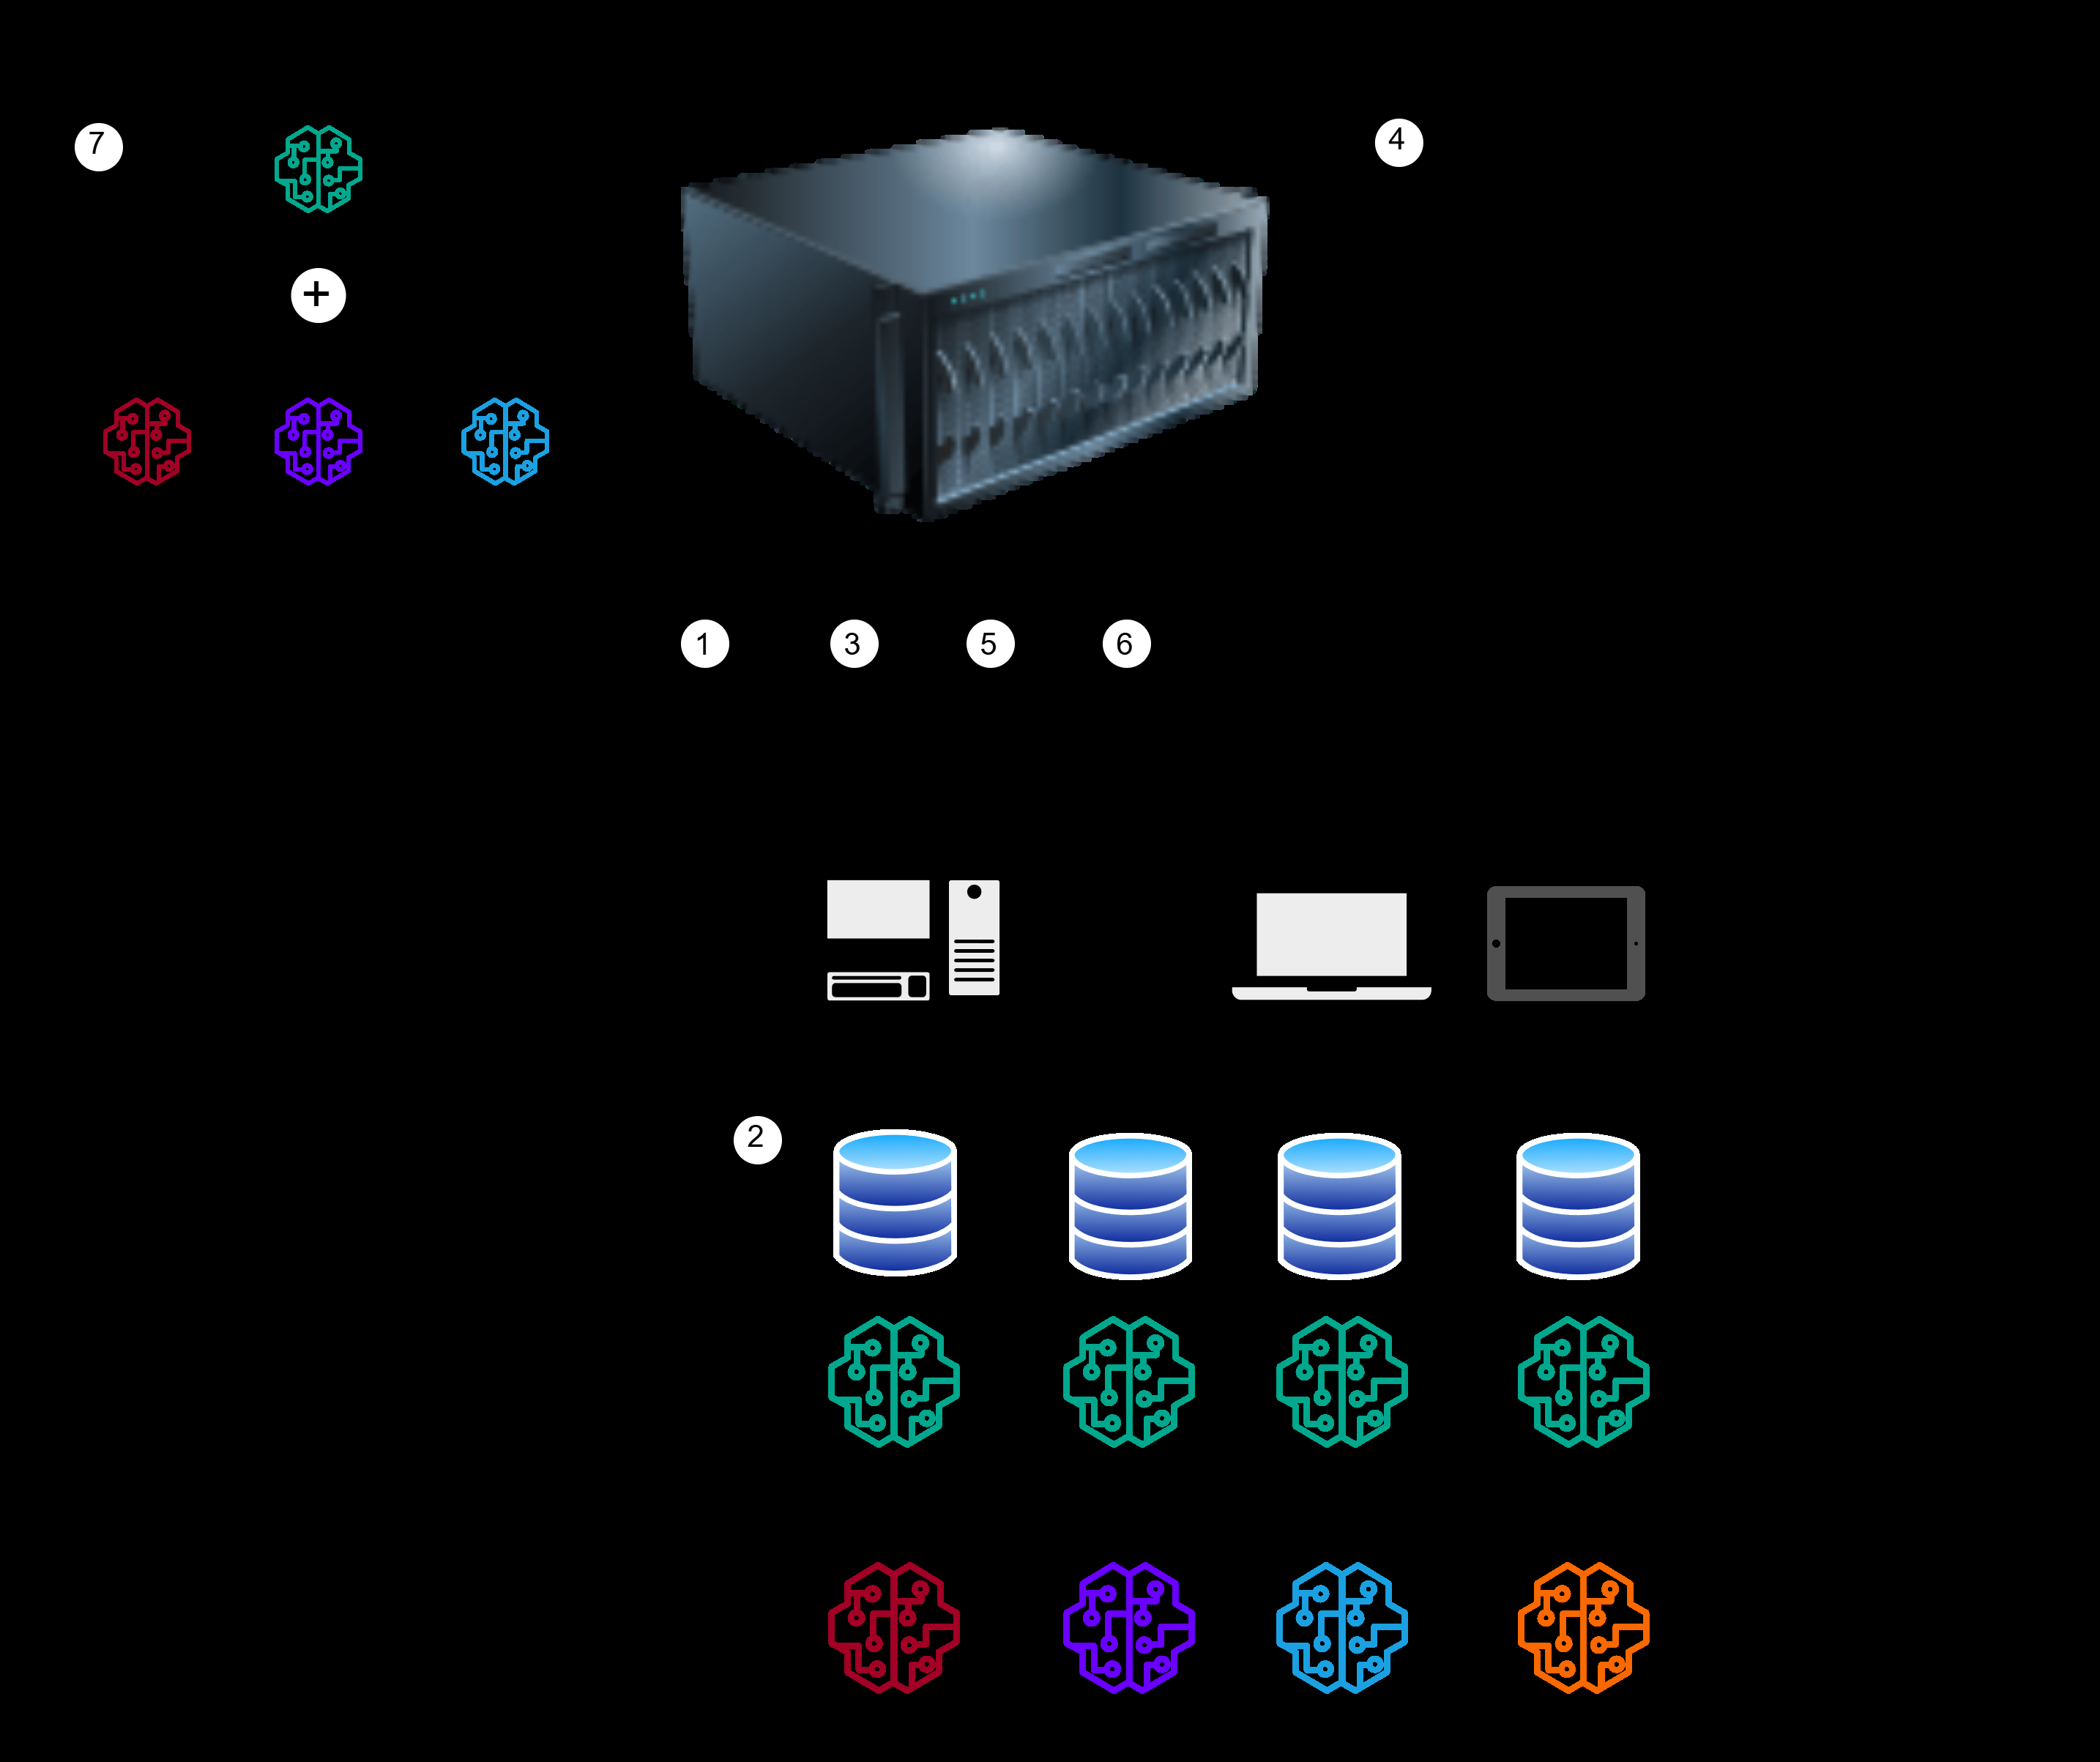
\includegraphics[width=0.78\textwidth]{figs/fig2.png}
\caption{Proposed framework architecture. Step numbers follow the protocol in Section~\ref{sec4.1}.}\label{fig:arch}
\end{figure}

\subsection{Local scoring and KL utility}\label{sec4.2}
The Kullback--Leibler (KL) divergence \citep{kullback1951} of a distribution $P$ from a reference distribution $Q$ is $\mathrm{KL}(P\Vert Q)=\sum_{c}P(c)\log\frac{P(c)}{Q(c)}$; it is nonnegative, zero only when $P=Q$, and asymmetric. For a classification task with label set $\mathcal{Y}$, client $i$ compares the class probabilities $P_i^t(\cdot\mid x)$ predicted by its model after local training with the probabilities $Q^t(\cdot\mid x)$ predicted by the unchanged global model received at the start of round $t$. Both are evaluated on the same client-local scoring examples. The per-example divergence is
\begin{equation}\label{eq:kld}
d_i^t(x)=\sum_{c\in\mathcal{Y}}P_i^t(c\mid x)\log\frac{P_i^t(c\mid x)}{Q^t(c\mid x)} ,
\end{equation}
the KL divergence of the local from the global prediction. The scoring examples are divided into $B$ nonempty batches $X_{i,b}^t$, $b=1,\dots,B$. The batch score and the example-weighted client score are
\begin{equation}\label{eq:klb}
\mathrm{KL}_{i,b}^t=\frac{1}{|X_{i,b}^t|}\sum_{x\in X_{i,b}^t}d_i^t(x),
\end{equation}
\begin{equation}\label{eq:kl}
\KL_i^t=\frac{\sum_{b=1}^{B}|X_{i,b}^t|\,\mathrm{KL}_{i,b}^t}{\sum_{b=1}^{B}|X_{i,b}^t|},
\end{equation}
so every scoring example has equal weight. The unweighted mean and sample variance of the batch scores are
\begin{equation}\label{eq:klmean}
\overline{\mathrm{KL}}_i^t=\frac{1}{B}\sum_{b=1}^{B}\mathrm{KL}_{i,b}^t,
\end{equation}
\begin{equation}\label{eq:var}
\sigma_i^2=\frac{1}{B-1}\sum_{b=1}^{B}\bigl(\mathrm{KL}_{i,b}^t-\overline{\mathrm{KL}}_i^t\bigr)^2 .
\end{equation}

The quantity $\KL_i^t$ measures the post-training \emph{disagreement} between the local and global predictions. Despite the symbol $\Delta$, it is not a before-and-after reduction in divergence, and a large value is not by itself evidence that aggregating the client's update would improve the global model: under non-IID data, local drift can also be harmful \citep{li2020,wang2020}. We use $\KL_i^t$ as a heuristic indicator of how much new, locally learnable information a client holds, and we do not claim that it predicts the held-out loss change of aggregation; that relationship was not tested (Section~\ref{sec:limits}). The variance $\sigma_i^2$ measures differences between scoring batches. It does not separate noisy data from legitimate heterogeneity or rare classes, and a consistently misleading client can have low between-batch variance. The sample variance requires $B\ge 2$ nonempty batches; for fewer batches it is undefined and is not silently replaced by zero. The batch count, sampling procedure and batch sizes must be specified for the score to be reproducible; the values used in the original experiments were not recorded (Section~\ref{sec:scope}).

\subsection{Idle-round fairness}\label{sec4.3}
Let $r_i^t$ count the consecutive committed rounds before round $t$ in which client $i$ was not selected, with $r_i^1=0$, and let $\bar r^t$ be the population mean, with $\bar r^1=0$. The server maintains the fairness priority
\begin{equation}\label{eq:fair}
F_i^t=1+\frac{r_i^t}{1+\bar r^t},
\end{equation}
which expresses waiting time relative to the population mean \citep{xu2024}. The $+1$ in the denominator avoids division by zero in the first round or when all clients were just selected. After each committed round, the counters and their mean are updated:
\begin{equation}\label{eq:idle}
r_i^{t+1}=\begin{cases}0, & i\in C_k^t,\\ r_i^t+1, & i\notin C_k^t,\end{cases}
\end{equation}
\begin{equation}\label{eq:rbar}
\bar r^{t+1}=\frac{1}{N}\sum_{i=1}^{N}r_i^{t+1}.
\end{equation}
For a fixed population, $1\le F_i^t<N+1$. Selection resets a counter to zero and non-selection increments it by one. The rule does not impose a maximum waiting time.

\subsection{Utility--fairness controller and fitness}\label{sec4.4}
The utility--fairness mixing coefficient $a_i^t\in[0,1]$ is initialised as $a_i^0=0.5$ and updated by
\begin{equation}\label{eq:a}
a_i^t=\operatorname{clip}\!\left(\beta a_i^{t-1}+(1-\beta)\frac{\nu^t\bigl(\KL_i^t-F_i^t\bigr)}{\lambda F_i^t+\bigl|\nu^t\bigl(\KL_i^t-F_i^t\bigr)\bigr|},\,0,\,1\right),
\end{equation}
where $\operatorname{clip}(x,0,1)=\min\{1,\max\{0,x\}\}$, $\beta=0.9$ and $\lambda=1$. Because $F_i^t\ge 1$ and $\lambda>0$, the denominator is strictly positive. The update smooths toward a signed feedback target in $[-1,1]$ and then clips; its sign depends jointly on $\nu^t$ and $\KL_i^t-F_i^t$, so a positive $\nu^t$ alone does not imply an increase of $a_i^t$. The priority score, the raw stability score and the fitness are
\begin{equation}\label{eq:prio}
\Pi_i^t=a_i^t\,\KL_i^t+(1-a_i^t)\,F_i^t,
\end{equation}
\begin{equation}\label{eq:s}
s_i^t=\KL_i^t-\mu\,\sigma_i^2,\qquad \mu\ge 0,
\end{equation}
\begin{equation}\label{eq:fit}
\Fit_i^t=\Pi_i^t-\mu\,\sigma_i^2 .
\end{equation}

Two properties of this design should be stated plainly. First, Eq.~\eqref{eq:prio} combines $a_i^t\KL_i^t$ and $(1-a_i^t)F_i^t$ on their original numerical scales. Since $F_i^t\ge 1$ while $\KL_i^t$ can be much smaller than one, the fairness term can dominate the priority over most of the range of $a_i^t$, which limits the practical influence of the controller; rescaling both terms to a common range before mixing would address this but was not evaluated. Second, Eq.~\eqref{eq:a} is a bounded exponential-moving-average feedback rule. It is not a Lyapunov function, and we provide no stability proof, convergence rate or fairness bound for FedFACS; the Lyapunov reference \citep{chaudhari2002} is cited only for the qualitative idea of feedback regulation.

\subsection{Convergence feedback}\label{sec4.5}
The validation-loss reduction of a completed round is
\begin{equation}\label{eq:rho}
\rho^t=\frac{L_{\mathrm{global}}^{t-1}-L_{\mathrm{global}}^{t}}{L_{\mathrm{global}}^{t-1}},\qquad L_{\mathrm{global}}^{t-1}>0,
\end{equation}
where $L_{\mathrm{global}}^0$ is the validation loss of the initial model. Selection in round $t$ uses $\rho^{t-1}$ and not the loss of its own candidate aggregate. We initialise $\rho^0=0$, $\nu^1=0$ and $\Omega^2=0$. With $\beta_{\mathrm{ref}}=0.9$, the causal reference and the deviation signal are
\begin{equation}\label{eq:omega}
\Omega^t=\beta_{\mathrm{ref}}\,\Omega^{t-1}+(1-\beta_{\mathrm{ref}})\,\rho^{t-2}\quad(t\ge 3),\qquad \Omega^2=0,
\end{equation}
\begin{equation}\label{eq:nu}
\nu^t=\Omega^t-\rho^{t-1},\qquad t\ge 2 .
\end{equation}
A negative $\rho^t$ records a validation-loss increase and remains in the feedback calculation. A zero previous loss terminates before division, and nonfinite values invalidate the round. The reference is computed entirely from earlier completed FedFACS rounds and uses no competing baseline trajectory. When $\nu^t>0$ the recent loss reduction is below its smoothed history; the controller's response depends on Eq.~\eqref{eq:a} as discussed above.

\subsection{Cohort sizing}\label{sec4.6}
For each configuration we specify integer bounds $1\le C_{k,\min}\le C_{k,\max}\le N$. The integer cohort size, with half-up rounding, is
\begin{equation}\label{eq:cohort}
m_t=\min\Bigl\{C_{k,\max},\ \max\Bigl\{C_{k,\min},\ \Bigl\lfloor C_{k,\min}+(C_{k,\max}-C_{k,\min})\bigl[1-\operatorname{clip}(\rho^{t-1},0,1)\bigr]+\tfrac12\Bigr\rfloor\Bigr\}\Bigr\}.
\end{equation}
The clipped ratio is used only for cohort sizing; the signed $\rho^{t-1}$ is retained in the feedback of Eqs.~\eqref{eq:omega}--\eqref{eq:nu}. Initialisation, an unchanged loss and an increasing loss select $C_{k,\max}$; a complete loss reduction selects $C_{k,\min}$. The rule is a heuristic interpolation and is not shown to identify an optimal or minimal cohort. Under the synchronous fixed-population protocol, a missing candidate report cancels the attempt without changing the bounds.

\subsection{Stability-weighted aggregation}\label{sec4.7}
For the selected clients, we keep the positive part of each raw stability score and its cohort sum,
\begin{equation}\label{eq:splus}
s_{i,+}^t=\max(s_i^t,0),\qquad H^t=\sum_{j\in C_k^t}s_{j,+}^t,
\end{equation}
and normalise the positive parts when their sum is positive; otherwise we use registered sample-count weights:
\begin{equation}\label{eq:S}
S_i^t=\begin{cases}\dfrac{s_{i,+}^t}{H^t}, & H^t>0,\\[2ex] \dfrac{n_i}{\sum_{j\in C_k^t}n_j}, & H^t=0.\end{cases}
\end{equation}
For numerically stable evaluation of the first branch, scale by the largest positive score $\hat s^t=\max_{j\in C_k^t}s_{j,+}^t$ and set $z_i^t=s_{i,+}^t/\hat s^t$, so that $S_i^t=z_i^t/\sum_{j\in C_k^t}z_j^t$ for $\hat s^t>0$. Both branches give $S_i^t\ge 0$ and $\sum_{i\in C_k^t}S_i^t=1$, and the aggregate is Eq.~\eqref{eq:agg}. Frozen model tensors and nontrainable buffers retain their round-start global values. A selected client with $S_i^t=0$ incurs upload cost and resets its idle counter, but makes no direct contribution to that round's aggregate. The positive-part and fallback rules are design choices introduced to make the weights well defined, and their effect was not isolated experimentally.

\subsection{Validation and state commitment}\label{sec4.8}
After aggregation, the server evaluates the candidate aggregate's validation loss and stages $\rho^t$, $\Omega^{t+1}$, $\nu^{t+1}$, $r_i^{t+1}$ and $\bar r^{t+1}$. The model, feedback and counters are committed together only after all numerical and protocol checks pass. A failed pre-commit attempt discards the staged state while retaining the record of consumed resources. Reports and decisions carry run and round identifiers; duplicate or stale messages are rejected, and a lost post-commit acknowledgement is recovered from the committed server outcome. The committed model, $\bar r^{t+1}$ and $\nu^{t+1}$ are broadcast to all candidates for the next round.

\subsection{Algorithms}\label{sec4.9}
Algorithms~\ref{alg:client} and~\ref{alg:server} give one consistent account of a round. In Algorithm~\ref{alg:client}, local parameters are reset to the received global parameters at the start of every round, the scoring predictions are computed after local training on the same scoring examples with the unchanged global model, and idle counters are held by the server and updated only at commit.

\begin{algorithm}[t]
\caption{Client-side training and fitness evaluation (client $i$, round $t$)}\label{alg:client}
\begin{algorithmic}[1]
\Require global model $w_{\mathrm{global}}^t$; server state $(\nu^t,\bar r^t,r_i^t)$; local data $D_i$; epochs $E$; learning rate $\eta$; client-held $a_i^{t-1}$
\State $w_i^t\gets w_{\mathrm{global}}^t$ \Comment{reset at every round}
\For{each local epoch $1,\dots,E$}
  \For{each mini-batch $(x,y)\subset D_i$}
    \State $w_i^t\gets w_i^t-\eta\nabla f_i(w_i^t)$ on the mini-batch loss of Eq.~\eqref{eq:loss}
  \EndFor
\EndFor
\State compute $P_i^t(\cdot|x)$ with $w_i^t$ and $Q^t(\cdot|x)$ with $w_{\mathrm{global}}^t$ on the $B$ scoring batches
\State compute $\KL_i^t$ \eqref{eq:kl} and $\sigma_i^2$ \eqref{eq:var}
\State compute $F_i^t$ \eqref{eq:fair}, $a_i^t$ \eqref{eq:a}, $\Pi_i^t$ \eqref{eq:prio}, $s_i^t$ \eqref{eq:s}, $\Fit_i^t$ \eqref{eq:fit}
\State report $\Fit_i^t$ to the server
\If{the server selects client $i$}
  \State upload $w_i^t$, $s_i^t$ and $n_i$
\EndIf
\end{algorithmic}
\end{algorithm}

\begin{algorithm}[t]
\caption{Server-side selection, aggregation and state update}\label{alg:server}
\begin{algorithmic}[1]
\Require population $\mathcal{C}$, bounds $(C_{k,\min},C_{k,\max})$, rounds $T$; initial model $w_{\mathrm{global}}^1$ with loss $L^0_{\mathrm{global}}>0$
\State initialise $r_i^1=0$, $\bar r^1=0$, $\rho^0=0$, $\nu^1=0$, $\Omega^2=0$
\For{$t=1,\dots,T$}
  \State broadcast $w_{\mathrm{global}}^t$, $\nu^t$, $\bar r^t$ to all $N$ candidates
  \State receive $\{\Fit_i^t\}_{i\in\mathcal{C}}$
  \State compute $m_t$ by \eqref{eq:cohort} from $\rho^{t-1}$
  \State select $C_k^t$ by \eqref{eq:sel} (ties by ascending identifier)
  \State receive $(w_i^t,s_i^t,n_i)$ from $i\in C_k^t$
  \State compute $S_i^t$ by \eqref{eq:splus}--\eqref{eq:S} and aggregate by \eqref{eq:agg}
  \State evaluate the candidate aggregate on validation data; compute $\rho^t$ \eqref{eq:rho}, $\Omega^{t+1}$ \eqref{eq:omega}, $\nu^{t+1}$ \eqref{eq:nu}
  \State compute $r_i^{t+1}$ \eqref{eq:idle} and $\bar r^{t+1}$ \eqref{eq:rbar}
  \State commit model, $\rho^t$, $\Omega^{t+1}$, $\nu^{t+1}$ and counters together (Section~\ref{sec4.8})
\EndFor
\end{algorithmic}
\end{algorithm}

\subsection{Trust assumptions}\label{sec4.10}
FedFACS assumes that clients report fitness scores, stability scores and sample counts honestly. The server does not verify these self-reported values before using them for selection and aggregation weighting, so a client that misreports can influence which clients are selected and how updates are weighted. This assumption is shared by comparable score-based selectors, but it is not a property we establish. Verification mechanisms, such as cross-validated scoring, anomaly detection on reported scores or Byzantine-robust aggregation, are not part of the design. The only privacy property we claim is that raw training data remain on the clients; no further privacy analysis is provided. Our evaluation is of a synchronous, simulated setting with at most 100 clients.

%% ------------------------------------------------------------------
\section{Experimental evaluation}\label{sec5}

\subsection{Datasets and partitions}\label{sec5.1}
We use four public benchmarks. MNIST \citep{lecun2010} and Fashion-MNIST (FMNIST) \citep{xiao2017} each contain 60{,}000 training and 10{,}000 test $28\times28$ grayscale images in ten classes (handwritten digits and clothing items, respectively). CIFAR-10 \citep{krizhevsky2009} contains 60{,}000 $32\times32$ RGB images in ten classes. The COVID-19 Radiography database \citep{rahman2020} contains chest radiographs from three classes: COVID-19, normal and viral pneumonia.

Heterogeneity is modelled with four partitioning scenarios. In S1 the training data are distributed with a Dirichlet distribution $\mathrm{Dir}(\alpha)$, $\alpha\in\{0.1,0.5\}$, producing imbalance in both client size and label distribution; a smaller $\alpha$ means stronger skew \citep{iyer2023}. In S2 each client is randomly assigned data from two classes \citep{zhai2024}. In S3 noisy data are generated and distributed across clients with a noise level from 0\% to 45\% per client under IID conditions. In S4, three clients hold data from all ten classes with noise levels of 10\% or 20\%, and the remaining clients hold only nine classes with the noise pattern of S3, under non-IID conditions \citep{shi2023}. The type and randomisation of the label or feature corruption used in S3 and S4 were not recorded.

\subsection{Models, configurations and baselines}\label{sec5.2}
FedFACS was implemented in Python with PyTorch and torchvision using ResNet-18 \citep{he2016}. The first convolutional layer and layers~1--3 are frozen; layer~4 and the final fully connected layer are trained. The output layer has 10 units for MNIST, FMNIST and CIFAR-10 and 3 units for COVID-19. The pretraining checkpoint, image preprocessing, grayscale-channel handling, normalisation and batch-normalisation treatment were not recorded. Experiments ran on an NVIDIA RTX 3090 GPU with 32~GB of RAM.

The evaluation is split into three separately defined configurations, and results are interpreted only within a configuration, dataset, partition, architecture, budget and target.
\begin{itemize}
\item \textbf{Configuration A} follows \citet{zhai2024}: 100 clients, 200 rounds, 10 local epochs, batch size 32, $\beta=0.9$, a maximum sampling rate of 0.1, SGD with learning rate 0.05 (CIFAR-10) and 0.01 (MNIST, FMNIST). Compared methods are FedAvg, FedProx (proximal coefficient 0.1), Pow-D (10 highest-loss clients out of 20 sampled), DivFL and Zhai et al., under partitions S1 and S2.
\item \textbf{Configuration B} follows \citet{liu2025}: FMNIST and CIFAR-10 with 100 clients and COVID-19 with 30 clients; 100 rounds on FMNIST and 350 rounds on CIFAR-10 and COVID-19; learning rates 0.001, 0.1 and 0.01 for FMNIST, CIFAR-10 and COVID-19, respectively; S1 with $\alpha=0.5$. Random, Pow-D and AHIBCS draw 15 candidate clients per round at random and aggregate 10. The $(C_{k,\min},C_{k,\max})$ bounds used for FedFACS in this configuration were not recorded and are not those of the Configuration~A ablation.
\item \textbf{Configuration C}: learning rates 0.005 (CIFAR-10) and 0.01 (FMNIST), batch size 64, 20 local epochs, and early stopping after 20 consecutive rounds without improvement in the global loss; the data split used for this stopping rule was not recorded. Compared methods are Random, Greedy (highest reputation), RBFF \citep{song2022} and FairFedCS \citep{shi2023} (control parameter $\sigma=0.6$), under S3 and S4.
\end{itemize}
Ablations use Configuration~A. The specification of Section~\ref{sec4} uses $\lambda=1$ and $a_i^0=0.5$; the values used in the original experiments for $\lambda$ (which the original manuscript did not state), $a_i^0$, $\mu$ and $B$, and the cohort bounds in Configurations~B and~C, were not recorded.

\subsection{Metrics}\label{sec5.3}
\emph{Accuracy} is the fraction of correctly classified test samples. \emph{Round-to-target} is the first completed round at which accuracy reaches the declared target; a run that does not reach the target within its budget is recorded as not reached. Validation data are intended for threshold selection, early stopping and checkpoint selection, and the held-out test set for reporting; final-round, peak and validation-selected-checkpoint accuracy are different endpoints and are not interchangeable. For the results reported here, the data split used to evaluate round-to-target and whether reported accuracies are final-round or peak values were not recorded. \emph{Recall}, \emph{precision} and \emph{F1} are
\begin{equation}\label{eq:recall}
\mathrm{Recall}=\frac{TP}{TP+FN},\qquad \mathrm{Precision}=\frac{TP}{TP+FP},\qquad F1=\frac{2\,\mathrm{Precision}\,\mathrm{Recall}}{\mathrm{Precision}+\mathrm{Recall}},
\end{equation}
where $TP$, $FP$ and $FN$ are correctly detected, incorrectly predicted and missed positives \citep{yacouby2020}. The averaging convention (macro, micro or weighted) used for the values reported here was not recorded.
\emph{Cumulative uploads} count repeated selected-client submissions,
\begin{equation}\label{eq:ctotal}
C_{\mathrm{total}}(T)=\sum_{t=1}^{T}|C_k^t| .
\end{equation}
For an attempted round $t$, let $\mathrm{Comm}^t_{\mathrm{down}}$, $\mathrm{Comm}^t_{\mathrm{up}}$ and $\mathrm{Comm}^t_{\mathrm{aux}}$ be the model-download, update-upload and auxiliary application traffic. Total counted communication is
\begin{equation}\label{eq:btotal}
\mathrm{Comm}_{\mathrm{total}}(T)=\mathrm{Comm}_{\mathrm{setup}}+\mathrm{Comm}_{\mathrm{cal}}+\mathrm{Comm}_{\mathrm{final}}+\sum_{t\in\mathcal{R}(T)}\bigl(\mathrm{Comm}^t_{\mathrm{down}}+\mathrm{Comm}^t_{\mathrm{up}}+\mathrm{Comm}^t_{\mathrm{aux}}\bigr),
\end{equation}
where $\mathrm{Comm}_{\mathrm{setup}}$ is one-time setup traffic, $\mathrm{Comm}_{\mathrm{cal}}$ is calibration traffic (zero for FedFACS under the causal reference of Eq.~\eqref{eq:omega}, nonzero for any method that needs a prior calibration run), $\mathrm{Comm}_{\mathrm{final}}$ is final-model distribution traffic, and $\mathcal{R}(T)$ is the set of attempted rounds up to $T$, including partial and cancelled attempts. Eq.~\eqref{eq:btotal} defines the accounting; \emph{it was not measured in our experiments}, and cumulative uploads are only one component of it.
\emph{Jain's fairness index} \citep{shi2024,cho2020} is
\begin{equation}\label{eq:jfi}
\mathrm{JFI}=\frac{\bigl(\sum_{i=1}^{N}p_i/q_i\bigr)^2}{N\sum_{i=1}^{N}(p_i/q_i)^2},\qquad q_i=(\text{number of labels})\times(1-\text{fraction of noisy data}),
\end{equation}
where $p_i$ is the participation rate of client $i$ in aggregation, $N$ is the client population and $q_i$ is the quality of its local data \citep{shi2023}. Because it is applied to $p_i/q_i$, $\mathrm{JFI}=1$ means participation proportional to quality, which equals equal raw participation only if all $q_i$ are equal. The minimum possible value is $1/N$, and the threshold of 0.5 sometimes used for description is a convention, not a property of the index. An index between 0.5 and 1 does not imply that every client participates: with equal quality, serving 90 of 100 clients uniformly and never serving the other ten gives $0.9$. Part of any JFI difference may also reflect selection correlating with data quality rather than with participation equality.

\subsection{Scope of the reported results}\label{sec:scope}
The numerical results in Tables~\ref{tab:abl-acc}--\ref{tab:c} and Figs.~\ref{fig:radar}--\ref{fig:jfidiff} were produced by the original implementation, before the formulation in Section~\ref{sec4} was revised in response to peer review. That implementation, its configuration files and the exact data partitions are no longer available, so the experiments could not be repeated with the revised formulation. Section~\ref{sec4} corrects several definitions that were ill-defined or inconsistent as originally written: the idle-round update (Eq.~\ref{eq:idle}, whose original form never incremented a counter), the denominator of the mixing controller (Eq.~\ref{eq:a}), the convergence reference (Eqs.~\ref{eq:omega}--\ref{eq:nu}, which originally depended on a prior baseline run), the integer cohort rule (Eq.~\ref{eq:cohort}) and the aggregation weights (Eq.~\ref{eq:S}, where scores could originally be negative). We cannot verify which of these corrections the original implementation already followed. Where it followed the original equations, Tables~\ref{tab:abl-acc}--\ref{tab:c} describe a closely related but not identical procedure, and the revised procedure has not been evaluated. The results should therefore be read as evidence about the FedFACS design as originally implemented, not as a validation of every detail of Section~\ref{sec4}. Re-evaluating the revised specification with multiple seeds is the main item of future work (Section~\ref{sec:limits}). Each reported value is from a single run, with no uncertainty estimate.

\subsection{Results}\label{sec5.4}

\subsubsection{Ablation}
Configuration~A compares full FedFACS with FedFACS-A1, which uses a fixed cohort of ten and sample-count aggregation, and FedFACS-A2, which keeps adaptive cohort sizing over $[8,10]$ with sample-count aggregation. Both use the same selection score as the full method. The comparison therefore distinguishes combined cohort-sizing and aggregation choices; it does not isolate the effects of the KL utility, the fairness term, the variance penalty or the feedback controller. Tables~\ref{tab:abl-acc} and~\ref{tab:abl-rounds} show that the full method is the most accurate in eight of nine settings (FMNIST~S2: 83.80 vs 83.81 for A1) and reaches the target in the fewest rounds in eight of nine settings; the exception is FMNIST S1 ($\alpha=0.5$), where the full method needs 99 rounds against 97 for A1. FedFACS-A1 alone is slower than Zhai et al.\ on CIFAR-10 (47, 69, 117 versus 44, 62, 113 rounds) and on MNIST S2 (123 versus 116), so the observed gains cannot be attributed to the selection score alone. With cohort bounds of 8--10, adaptive sizing can lower the per-round cohort by at most 20\% relative to a fixed cohort of ten.

\begin{table}[t]
\caption{Accuracy (\%) of FedFACS and its ablated variants (Configuration~A, single run).}\label{tab:abl-acc}
\centering
\begin{tabular}{llccc}
\toprule
Dataset & Scenario & FedFACS-A1 & FedFACS-A2 & FedFACS\\
\midrule
CIFAR-10 & S1 ($\alpha=0.1$) & 46.89 & 46.70 & 47.07\\
 & S1 ($\alpha=0.5$) & 50.37 & 49.95 & 51.12\\
 & S2 & 46.92 & 46.61 & 47.33\\
MNIST & S1 ($\alpha=0.1$) & 98.23 & 98.12 & 98.52\\
 & S1 ($\alpha=0.5$) & 98.63 & 98.48 & 98.91\\
 & S2 & 97.75 & 97.61 & 98.11\\
FMNIST & S1 ($\alpha=0.1$) & 86.35 & 86.19 & 86.63\\
 & S1 ($\alpha=0.5$) & 88.35 & 87.91 & 88.95\\
 & S2 & 83.81 & 83.76 & 83.80\\
\bottomrule
\end{tabular}
\end{table}

\begin{table}[t]
\caption{Rounds to the target accuracy for FedFACS and its ablated variants (Configuration~A, single run).}\label{tab:abl-rounds}
\centering
\begin{tabular}{llccc}
\toprule
Dataset & Scenario & FedFACS-A1 & FedFACS-A2 & FedFACS\\
\midrule
CIFAR-10 & S1 ($\alpha=0.1$) & 47 & 44 & 40\\
 & S1 ($\alpha=0.5$) & 69 & 64 & 57\\
 & S2 & 117 & 115 & 110\\
MNIST & S1 ($\alpha=0.1$) & 67 & 62 & 58\\
 & S1 ($\alpha=0.5$) & 72 & 73 & 69\\
 & S2 & 123 & 117 & 115\\
FMNIST & S1 ($\alpha=0.1$) & 85 & 83 & 81\\
 & S1 ($\alpha=0.5$) & 97 & 103 & 99\\
 & S2 & 111 & 113 & 105\\
\bottomrule
\end{tabular}
\end{table}

\subsubsection{Configuration A: comparison with FedAvg, FedProx, Pow-D, DivFL and Zhai et al.}
Targets follow \citet{zhai2024}: 44\%, 48\% and 44\% on CIFAR-10, 97\%, 98\% and 97\% on MNIST, and 84\%, 87\% and 80\% on FMNIST for S1 ($\alpha=0.1$), S1 ($\alpha=0.5$) and S2, respectively; the FedFACS columns of Tables~\ref{tab:abl-rounds} and~\ref{tab:rounds} coincide, so the ablation uses the same targets. Table~\ref{tab:rounds} reports the rounds required, Fig.~\ref{fig:radar} summarises accuracy and Figs.~\ref{fig:cifar}--\ref{fig:fmnist} show the accuracy curves. Relative to Zhai et al., FedFACS needs fewer rounds in all nine settings: by 9.1\%, 8.1\% and 2.7\% on CIFAR-10, by 14.7\%, 5.5\% and 0.9\% on MNIST and by 4.7\%, 2.0\% and 2.8\% on FMNIST, computed from Table~\ref{tab:rounds}. The reduction is largest where target accuracy is reached early and smallest under the strongest skew. DivFL reaches the MNIST targets much faster under both S1 settings (28 and 35 rounds versus 58 and 69), and FedFACS trades this speed for higher final accuracy than DivFL: the original evaluation reports differences of 1.19, 0.74 and 1.98 on MNIST (it does not state whether these are absolute or relative). Entries equal to 200 equal the training budget; the original evaluation does not distinguish reaching a target in round 200 from not reaching it, so these entries should be read as ``not reached, or reached only at the budget limit''. FedFACS final accuracies are 47.07, 51.12 and 47.33 on CIFAR-10, 98.52, 98.91 and 98.11 on MNIST and 86.63, 88.95 and 83.80 on FMNIST (Table~\ref{tab:abl-acc}); the original evaluation reports differences over the best baseline of 0.48, 0.89 and 0.67 (CIFAR-10), 0.27, 0.31 and 0.22 (MNIST), and $+0.35$, $+0.85$ and $-0.2$ (FMNIST), again without stating absolute or relative units. On FMNIST S2 FedFACS is therefore marginally below the best baseline in accuracy. Cumulative aggregated clients (Fig.~\ref{fig:cum}) are lower than those of the best-performing baseline by roughly 4--12.5\% (CIFAR-10), 7--17\% (MNIST) and 2.3--5.8\% (FMNIST) according to the original evaluation.

\begin{table}[t]
\caption{Rounds required to reach the target accuracy: FedFACS versus baselines (Configuration~A, single run). Entries marked $\ddagger$ equal the 200-round budget.}\label{tab:rounds}
\centering
\small
\begin{tabular}{llcccccc}
\toprule
Dataset & Scenario & FedAvg & FedProx & Pow-D & DivFL & Zhai et al. & FedFACS\\
\midrule
CIFAR-10 & S1 ($\alpha=0.1$) & 91 & 197 & 97 & 72 & 44 & 40\\
 & S1 ($\alpha=0.5$) & 105 & 87 & 153 & 130 & 62 & 57\\
 & S2 & 135 & 148 & 125 & 200$^\ddagger$ & 113 & 110\\
MNIST & S1 ($\alpha=0.1$) & 118 & 131 & 100 & 28 & 68 & 58\\
 & S1 ($\alpha=0.5$) & 100 & 106 & 94 & 35 & 73 & 69\\
 & S2 & 145 & 169 & 135 & 200$^\ddagger$ & 116 & 115\\
FMNIST & S1 ($\alpha=0.1$) & 117 & 132 & 115 & 179 & 85 & 81\\
 & S1 ($\alpha=0.5$) & 128 & 116 & 124 & 161 & 101 & 99\\
 & S2 & 168 & 186 & 125 & 200$^\ddagger$ & 108 & 105\\
\bottomrule
\end{tabular}
\end{table}

\begin{figure}[t]
\centering
\begin{minipage}[t]{0.32\textwidth}\centering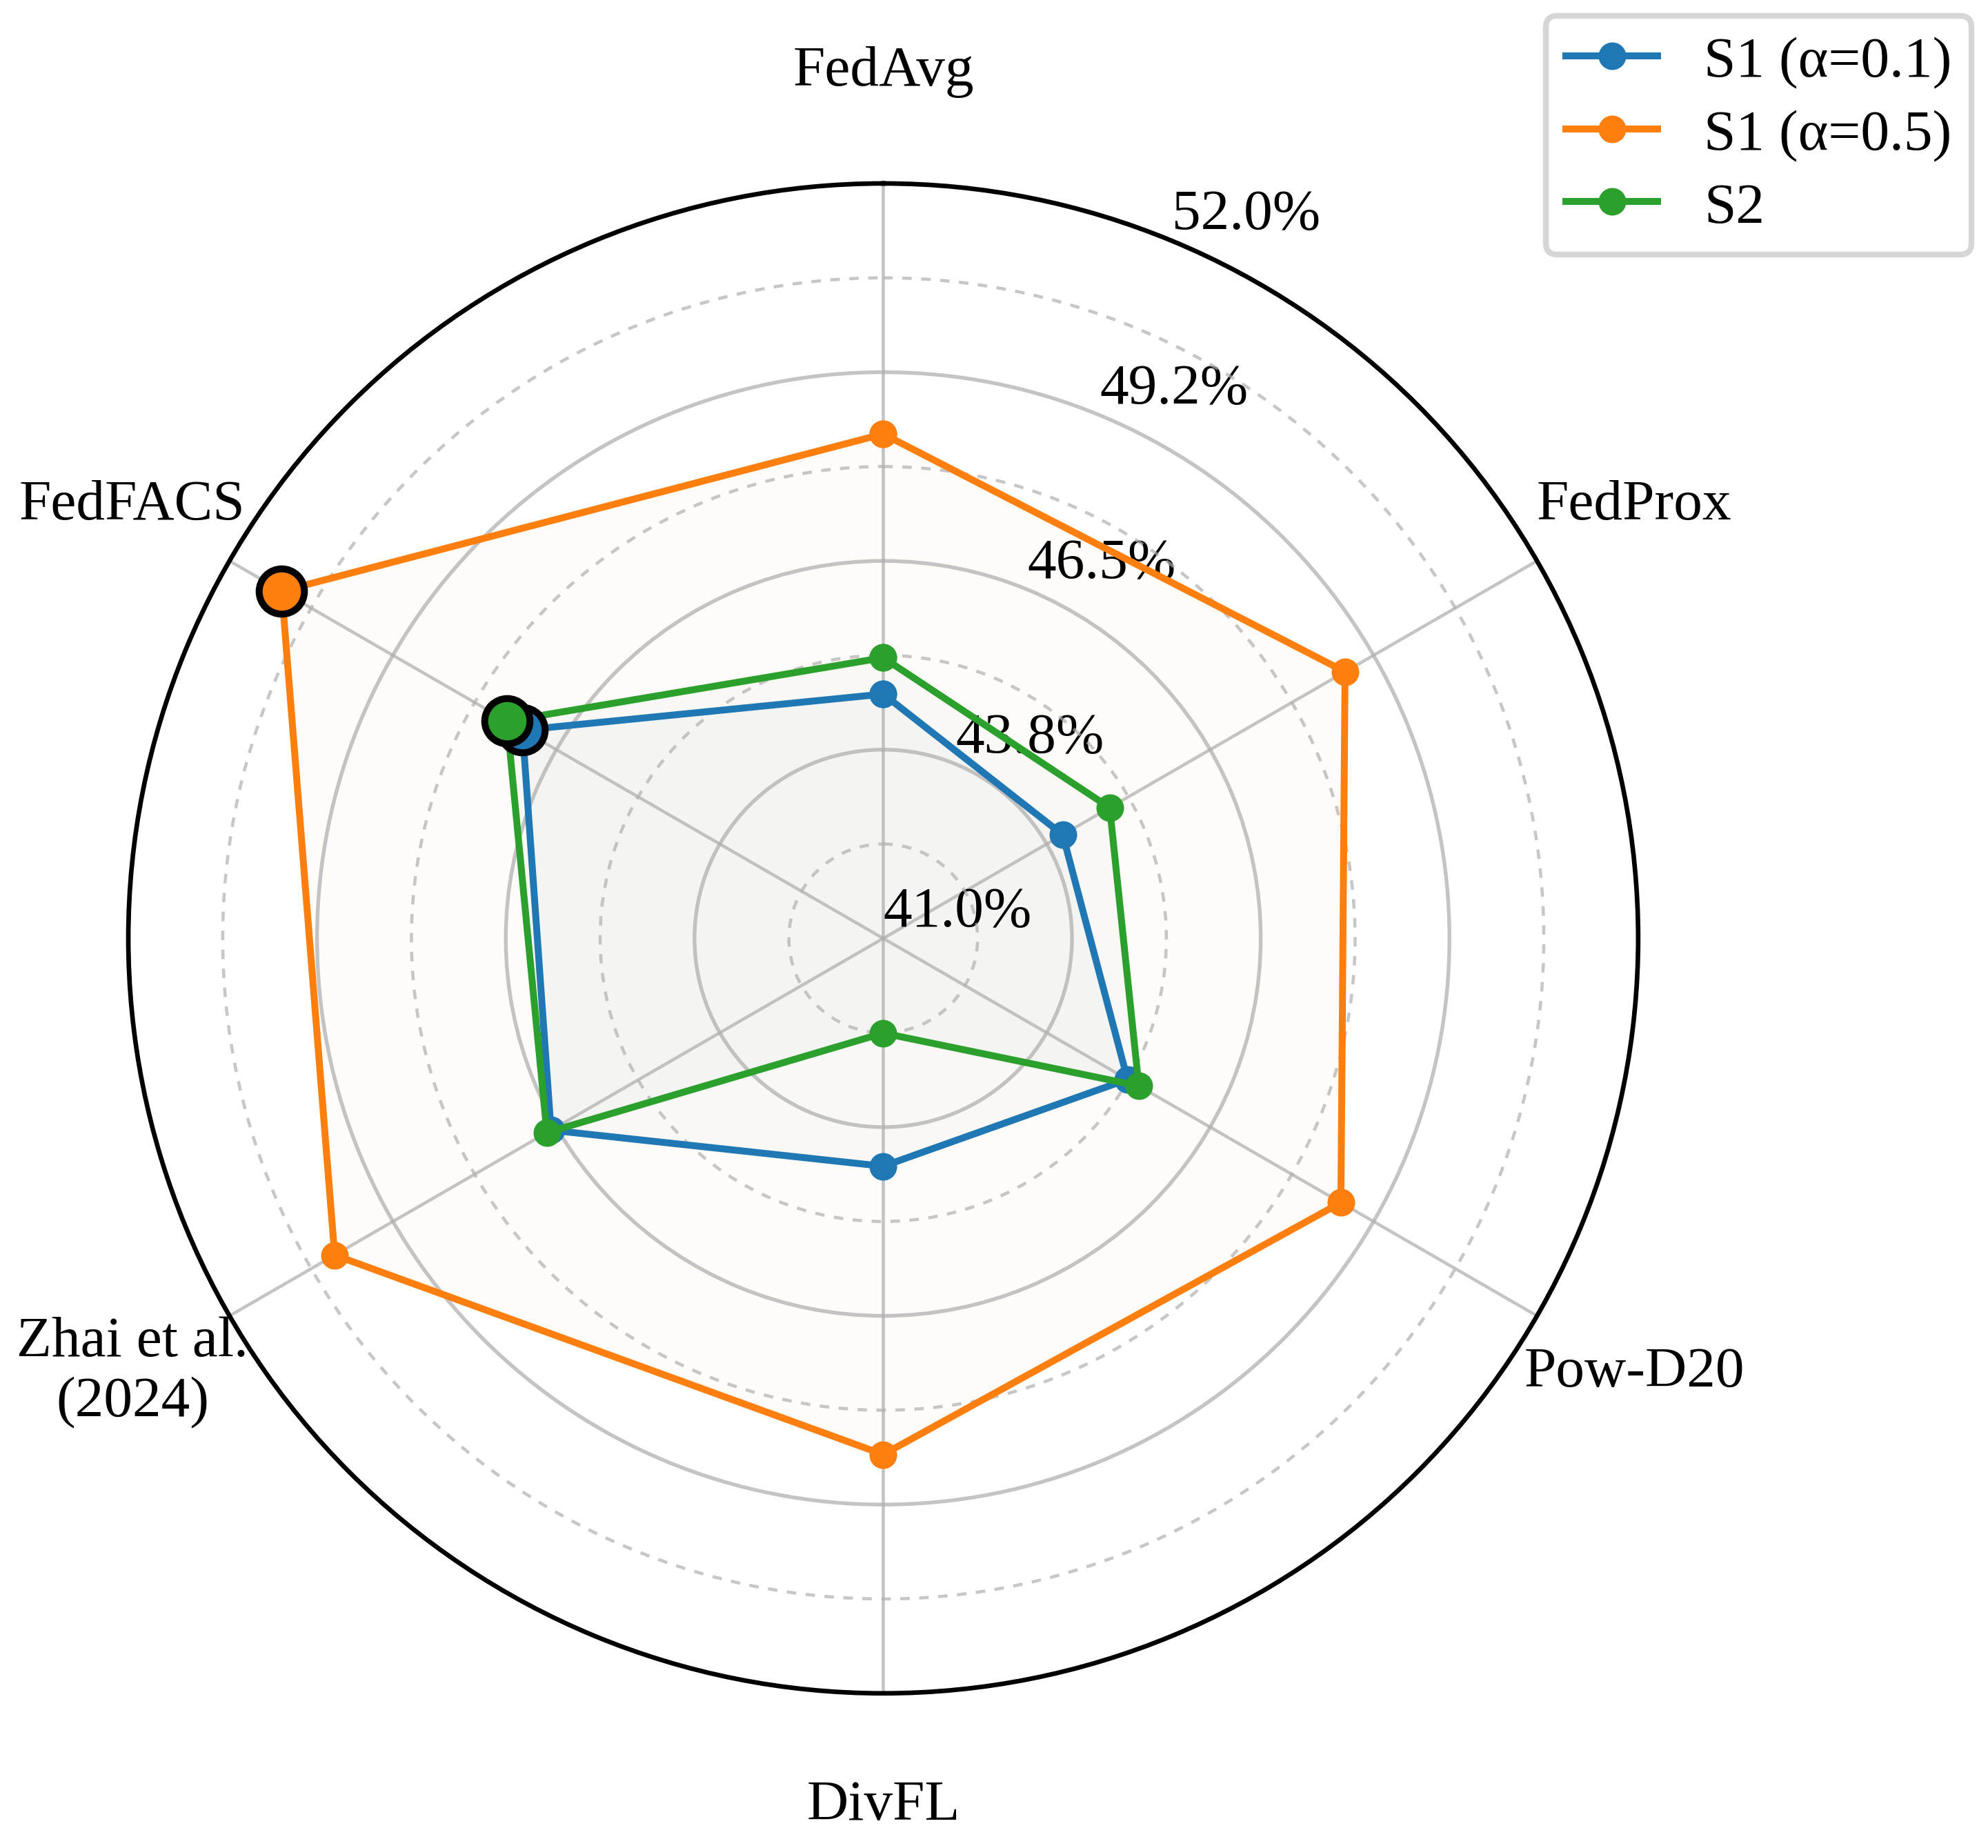
\includegraphics[width=\textwidth]{figs/fig3a.png}\\(a) CIFAR-10\end{minipage}\hfill
\begin{minipage}[t]{0.32\textwidth}\centering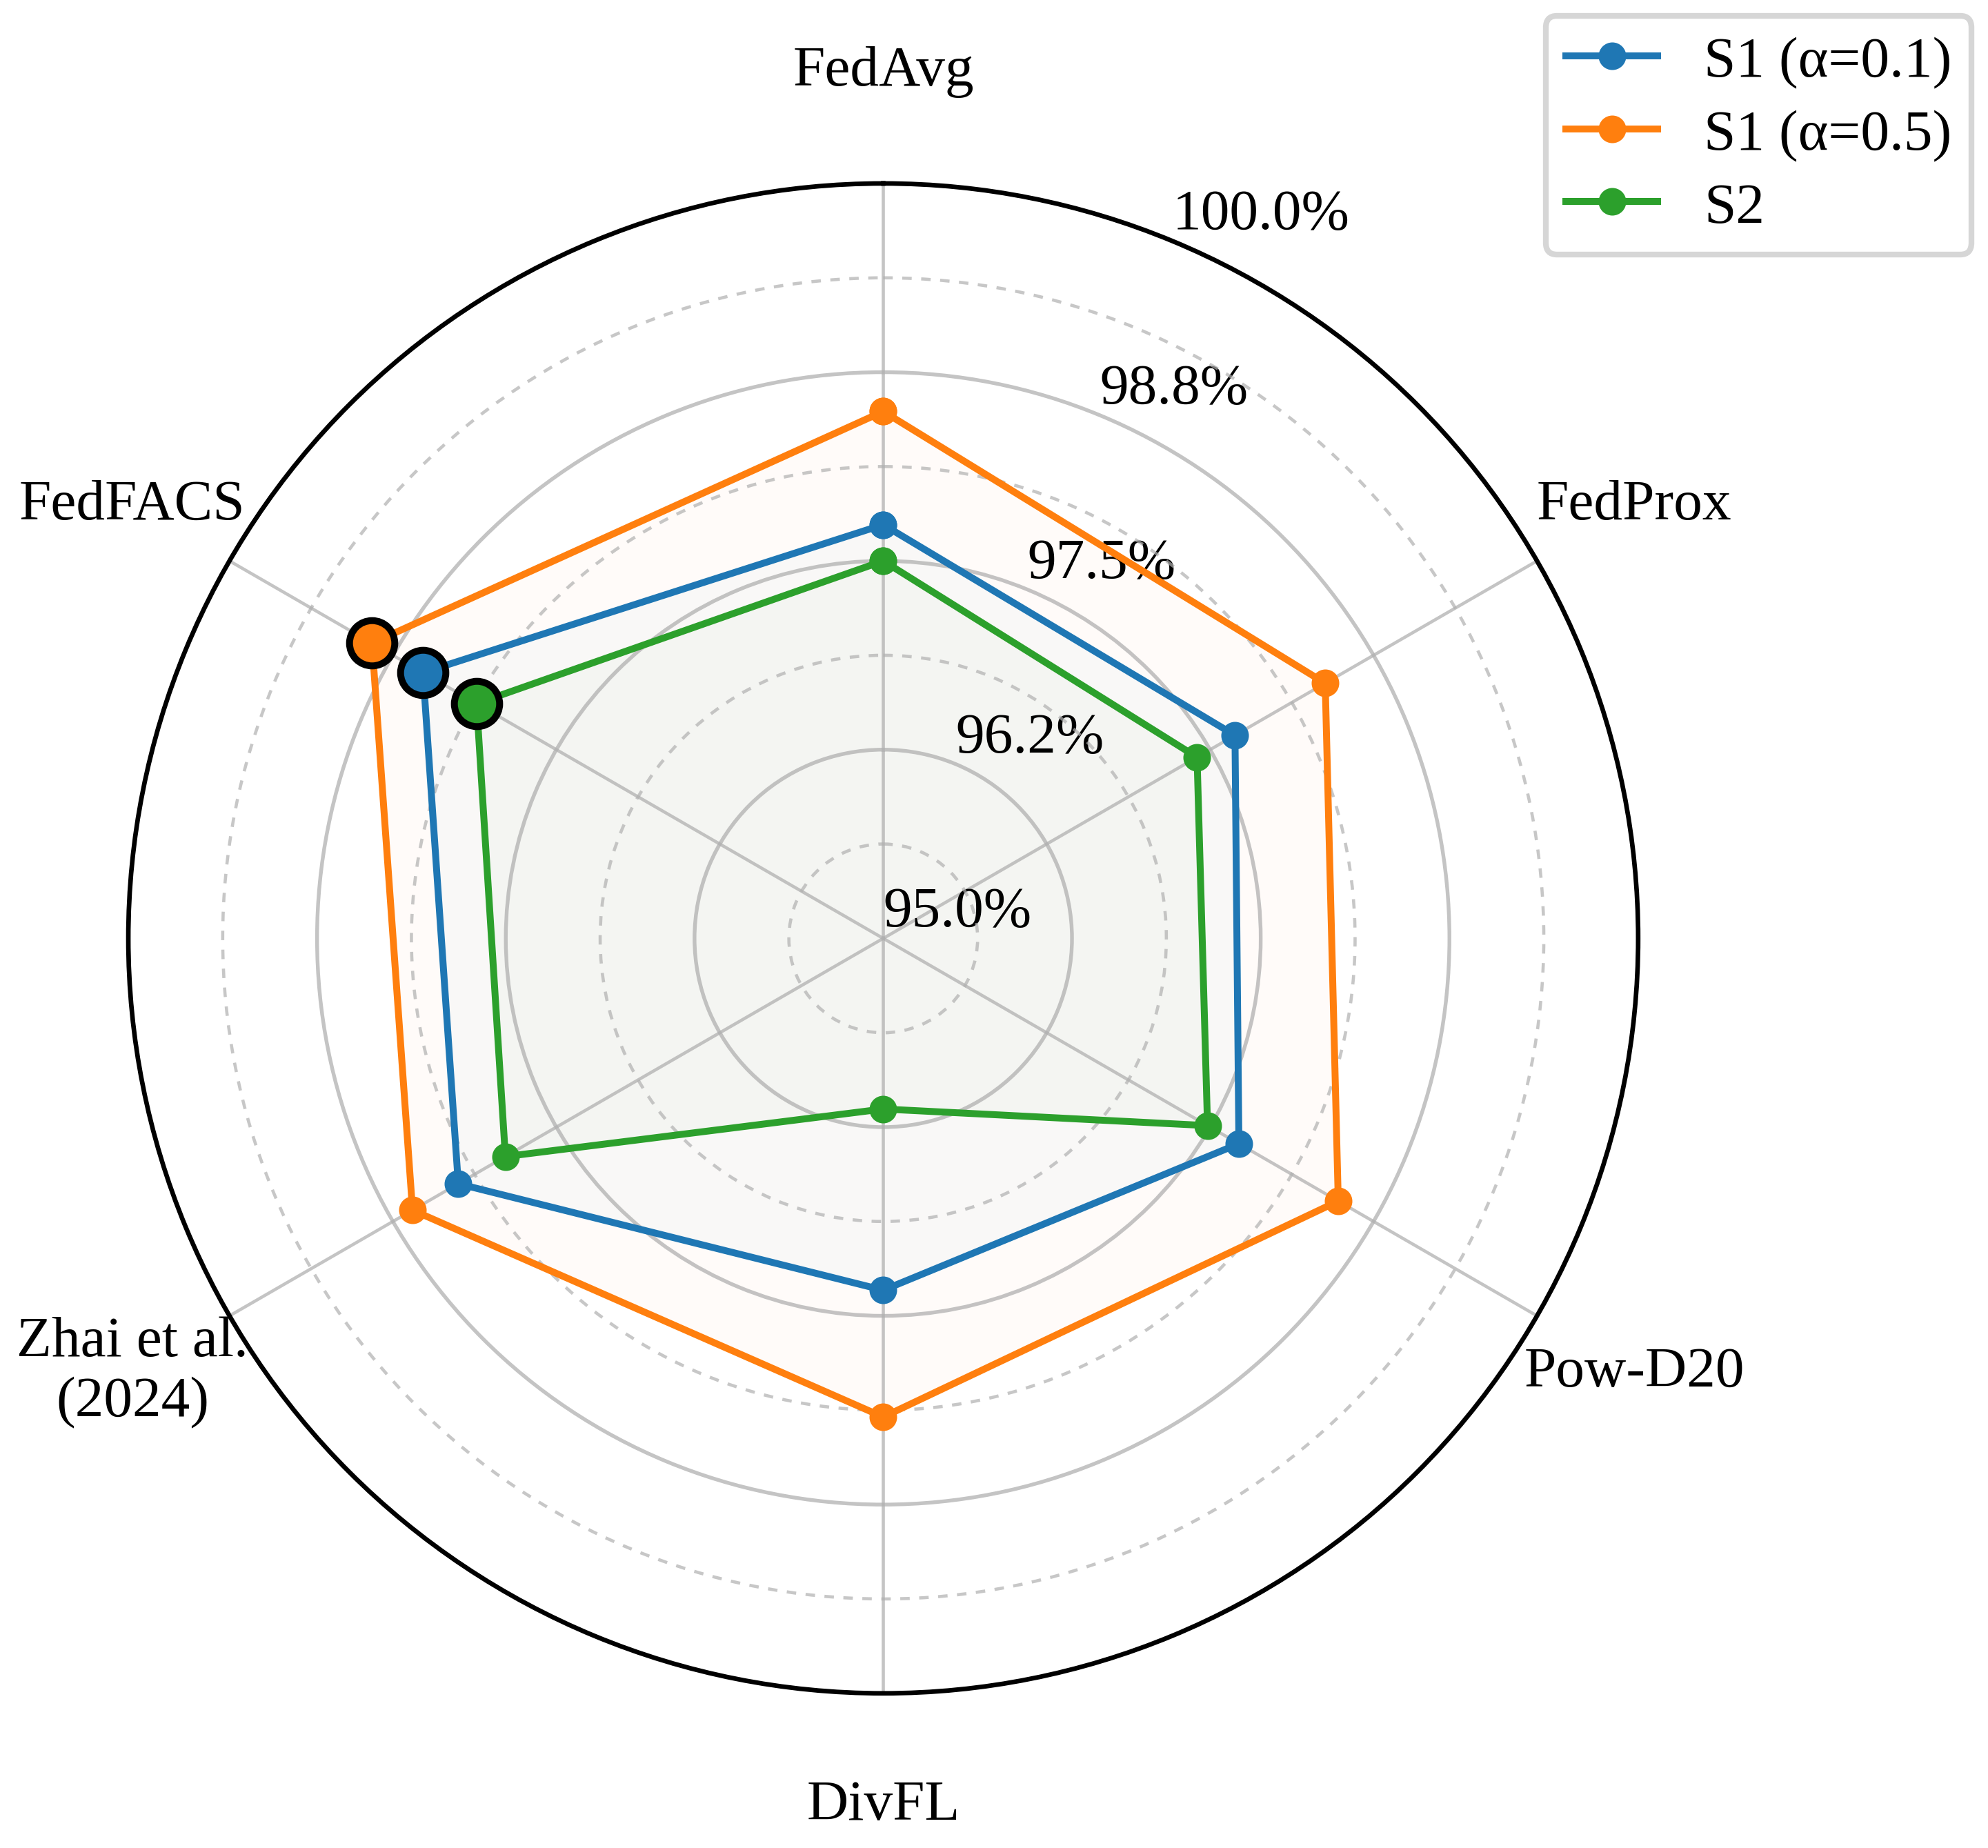
\includegraphics[width=\textwidth]{figs/fig3b.png}\\(b) MNIST\end{minipage}\hfill
\begin{minipage}[t]{0.32\textwidth}\centering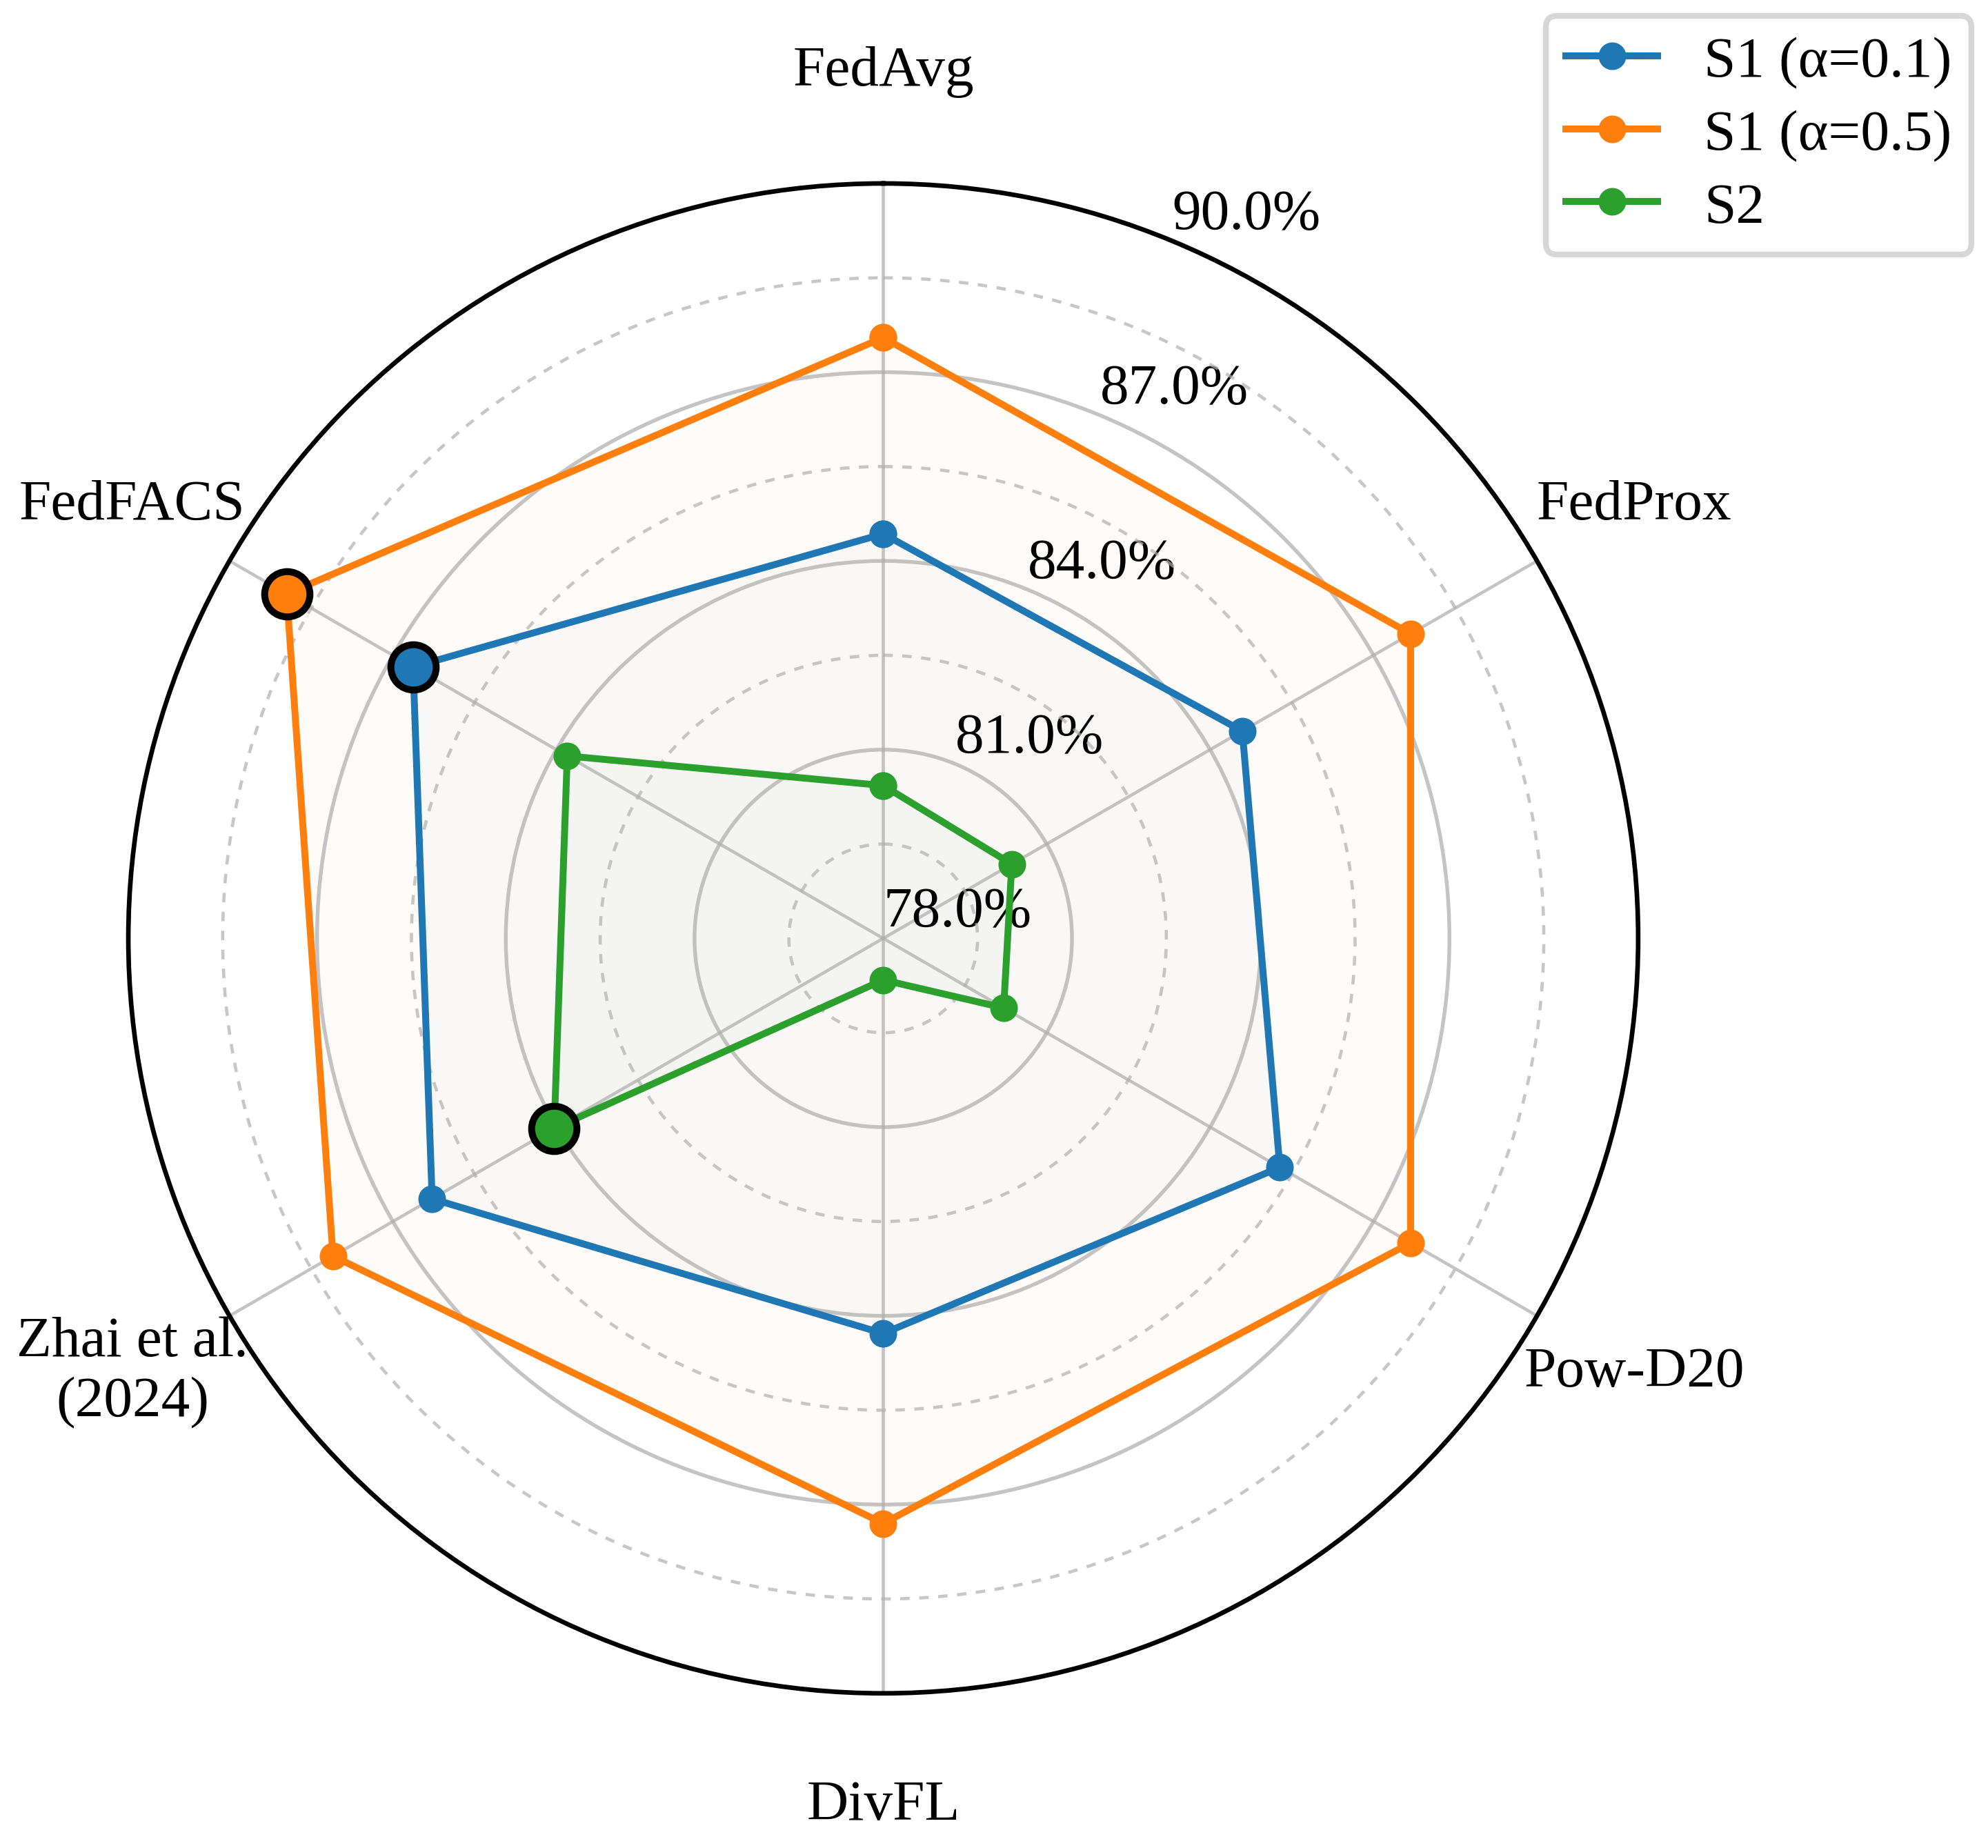
\includegraphics[width=\textwidth]{figs/fig3c.png}\\(c) FMNIST\end{minipage}
\caption{Classification accuracy of FedFACS and baseline methods under the heterogeneous scenarios, for CIFAR-10, MNIST and FMNIST. Outer axes are the compared methods and each curve is one scenario; markers highlight the best method in each scenario.}\label{fig:radar}
\end{figure}

\begin{figure}[t]
\centering
\begin{minipage}[t]{0.32\textwidth}\centering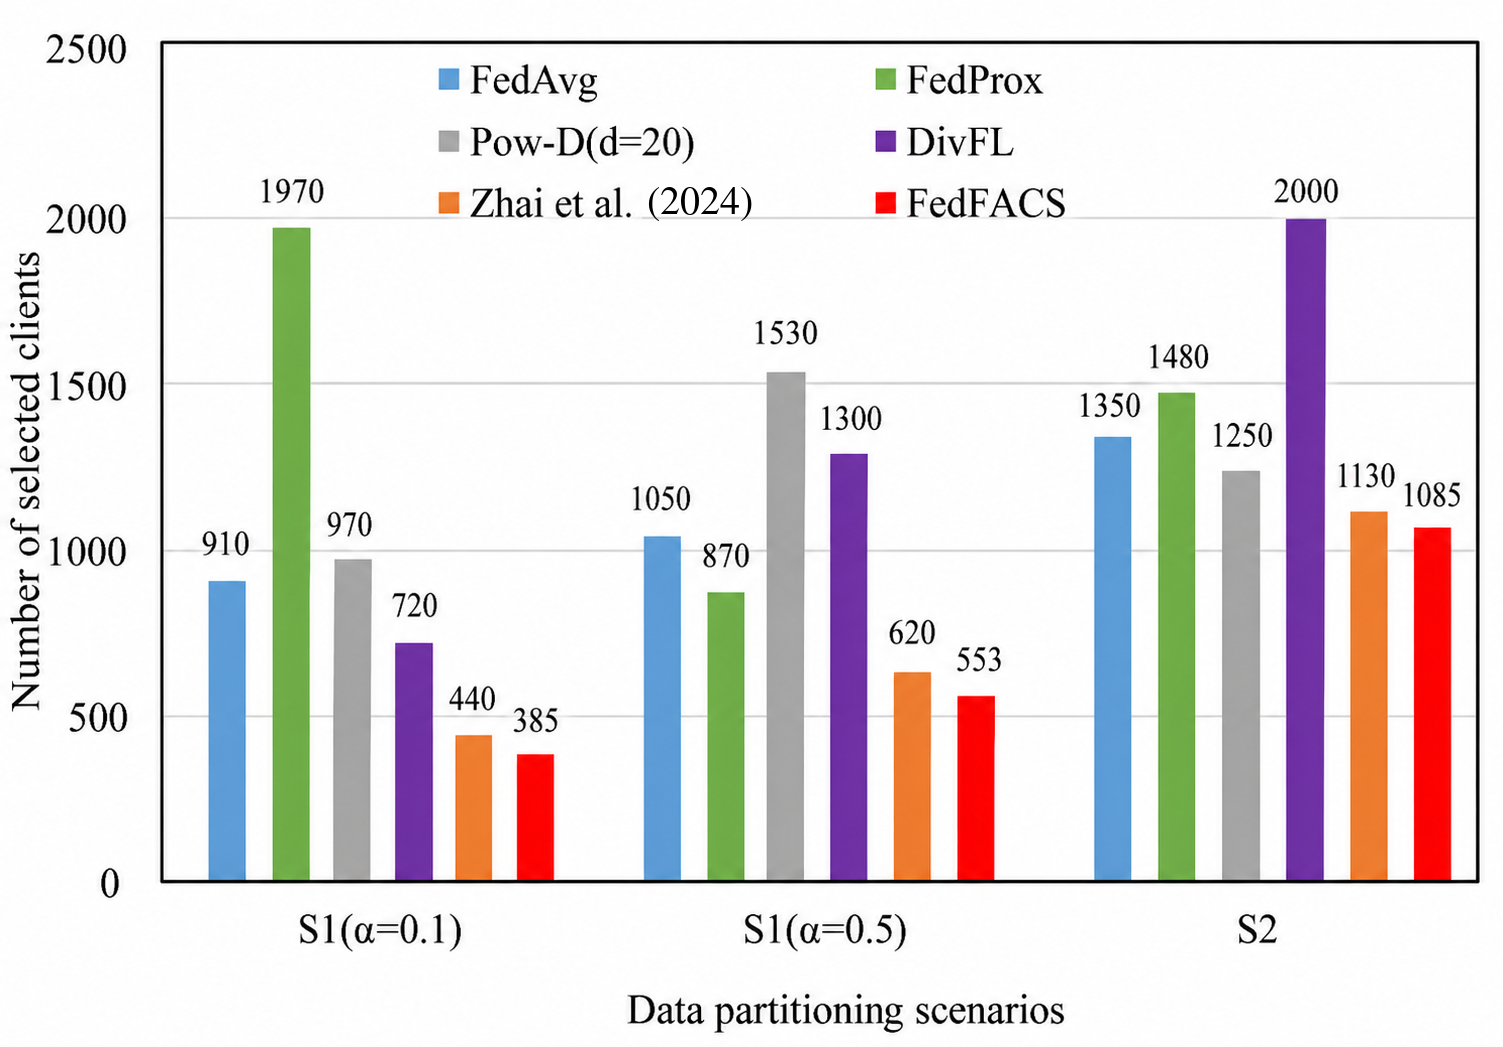
\includegraphics[width=\textwidth]{figs/fig4a.png}\\(a) CIFAR-10\end{minipage}\hfill
\begin{minipage}[t]{0.32\textwidth}\centering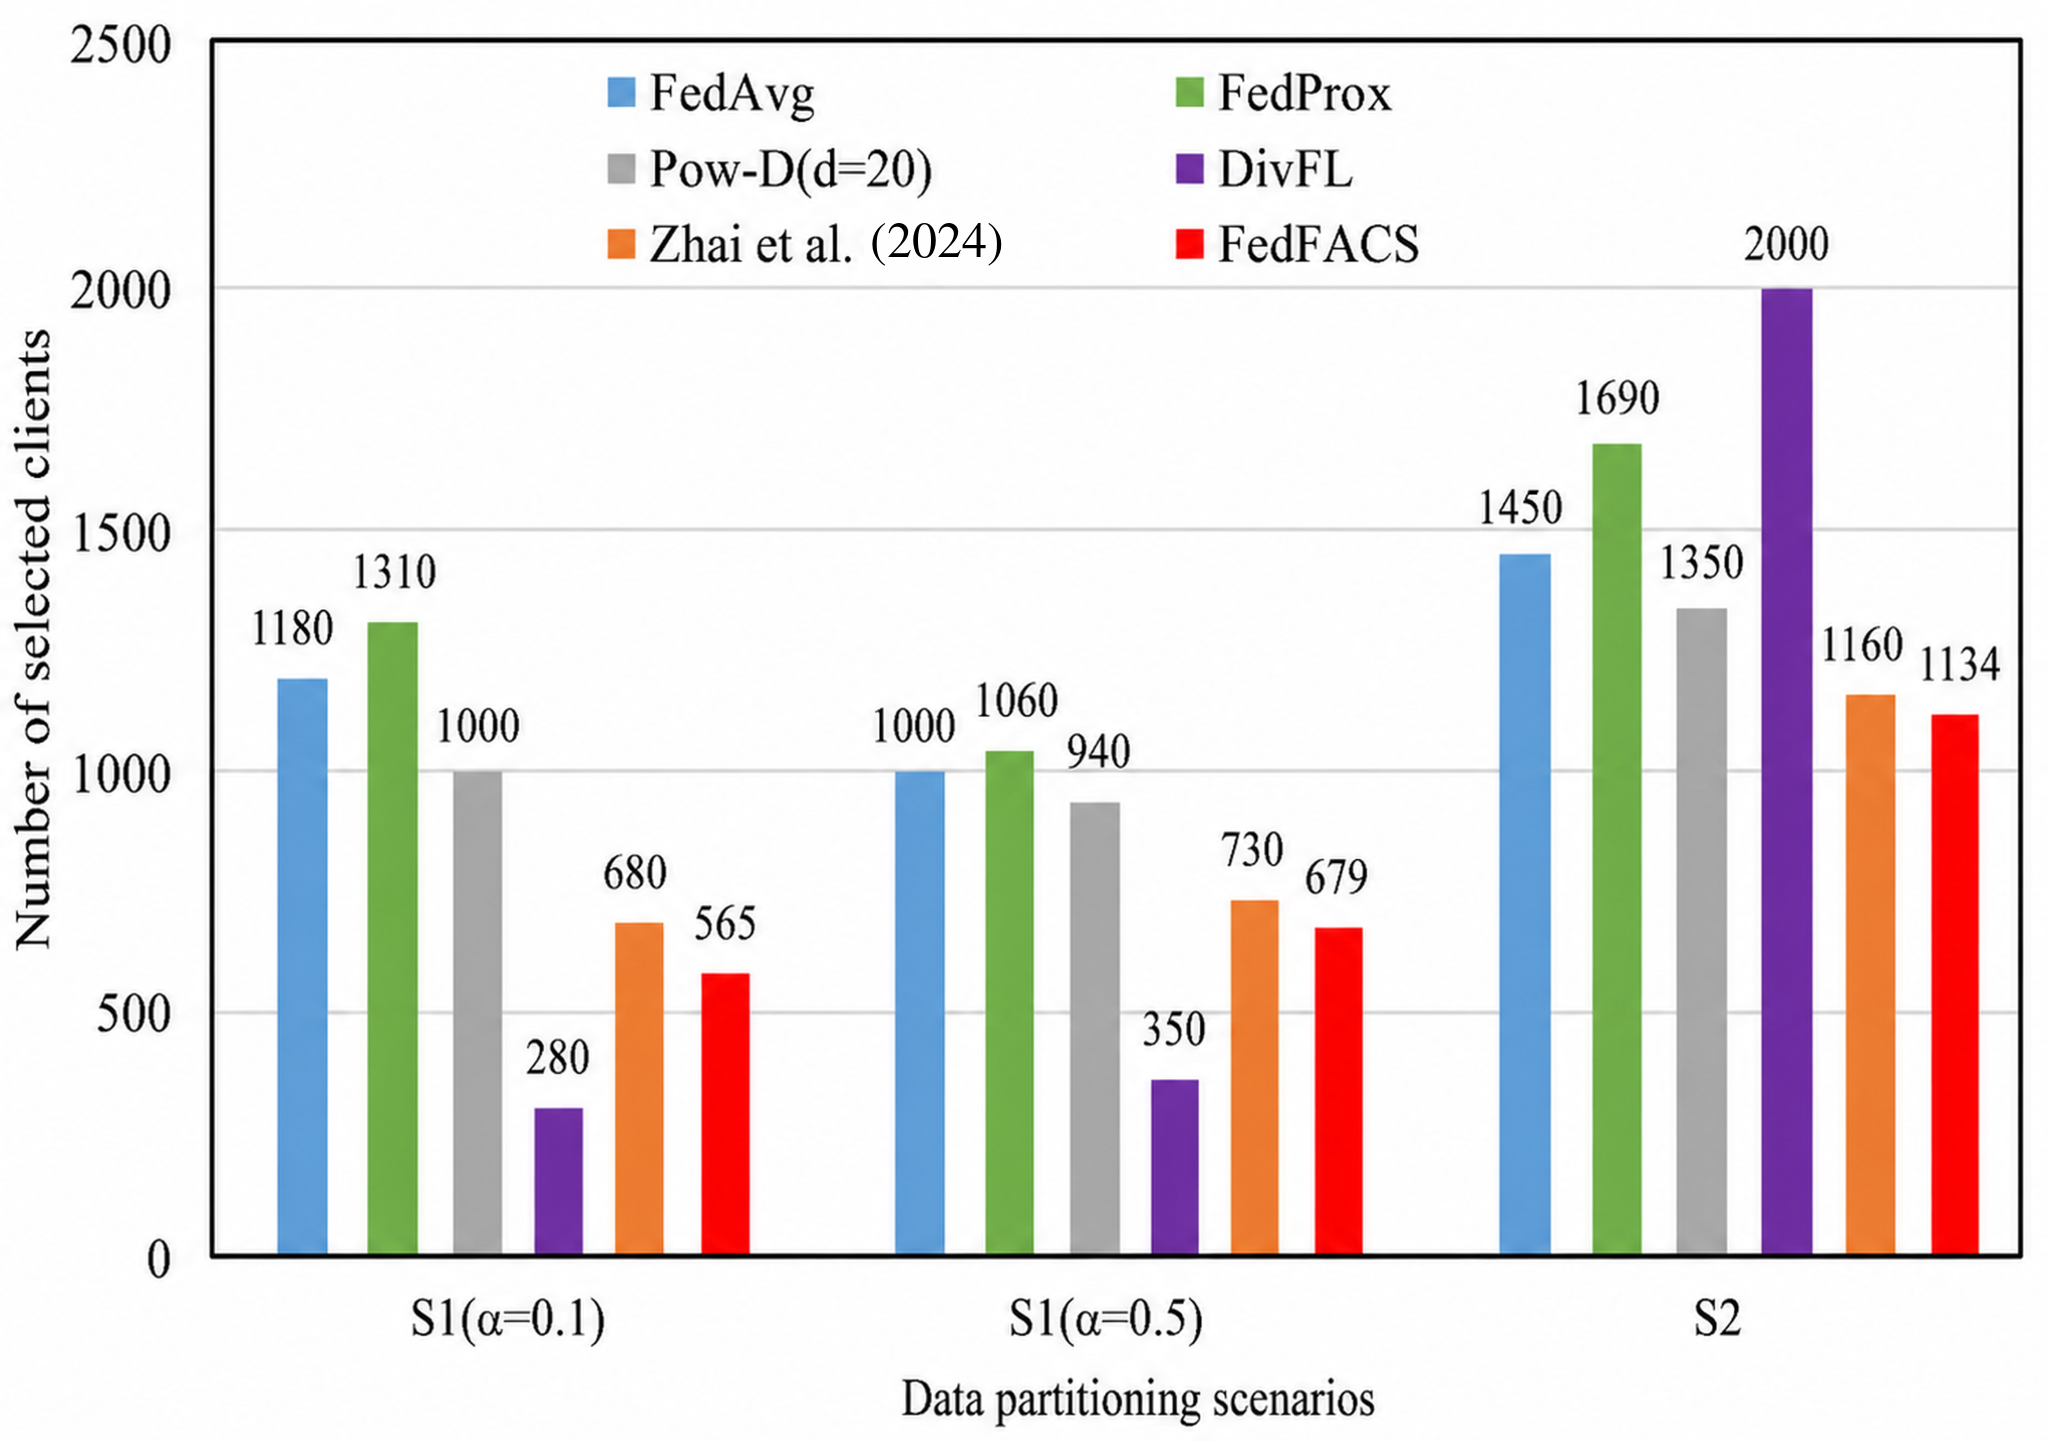
\includegraphics[width=\textwidth]{figs/fig4b.png}\\(b) MNIST\end{minipage}\hfill
\begin{minipage}[t]{0.32\textwidth}\centering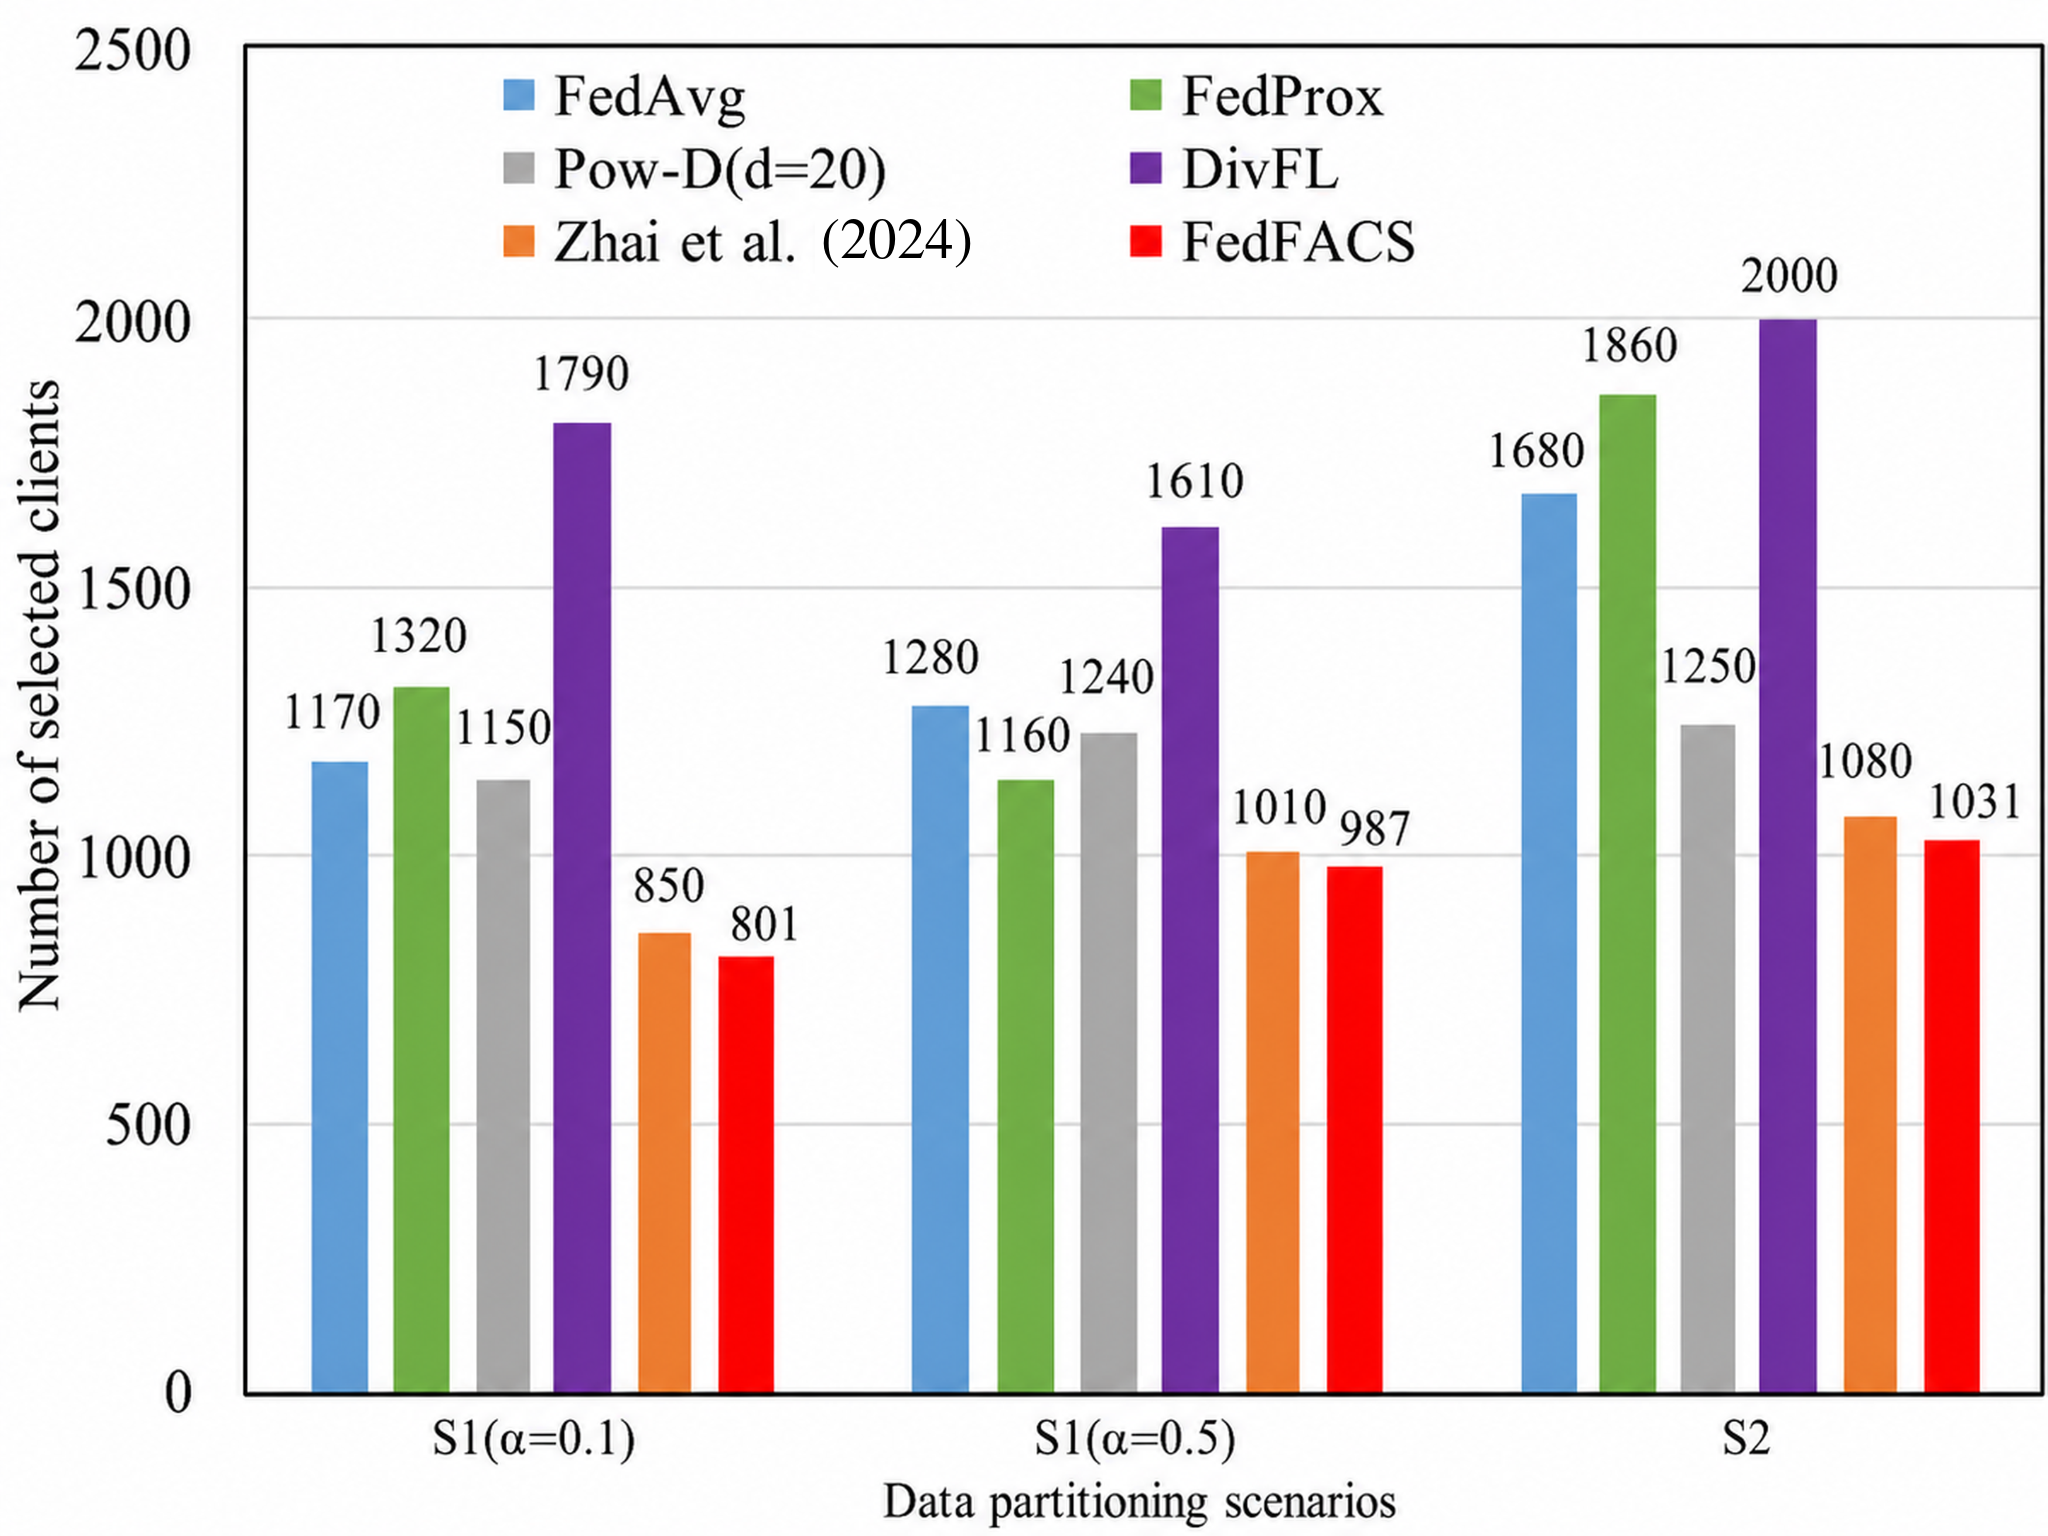
\includegraphics[width=\textwidth]{figs/fig4c.png}\\(c) FMNIST\end{minipage}
\caption{Cumulative number of selected clients required to reach the target accuracy in Scenarios~1 and~2.}\label{fig:cum}
\end{figure}

\begin{figure}[t]
\centering
\begin{minipage}[t]{0.32\textwidth}\centering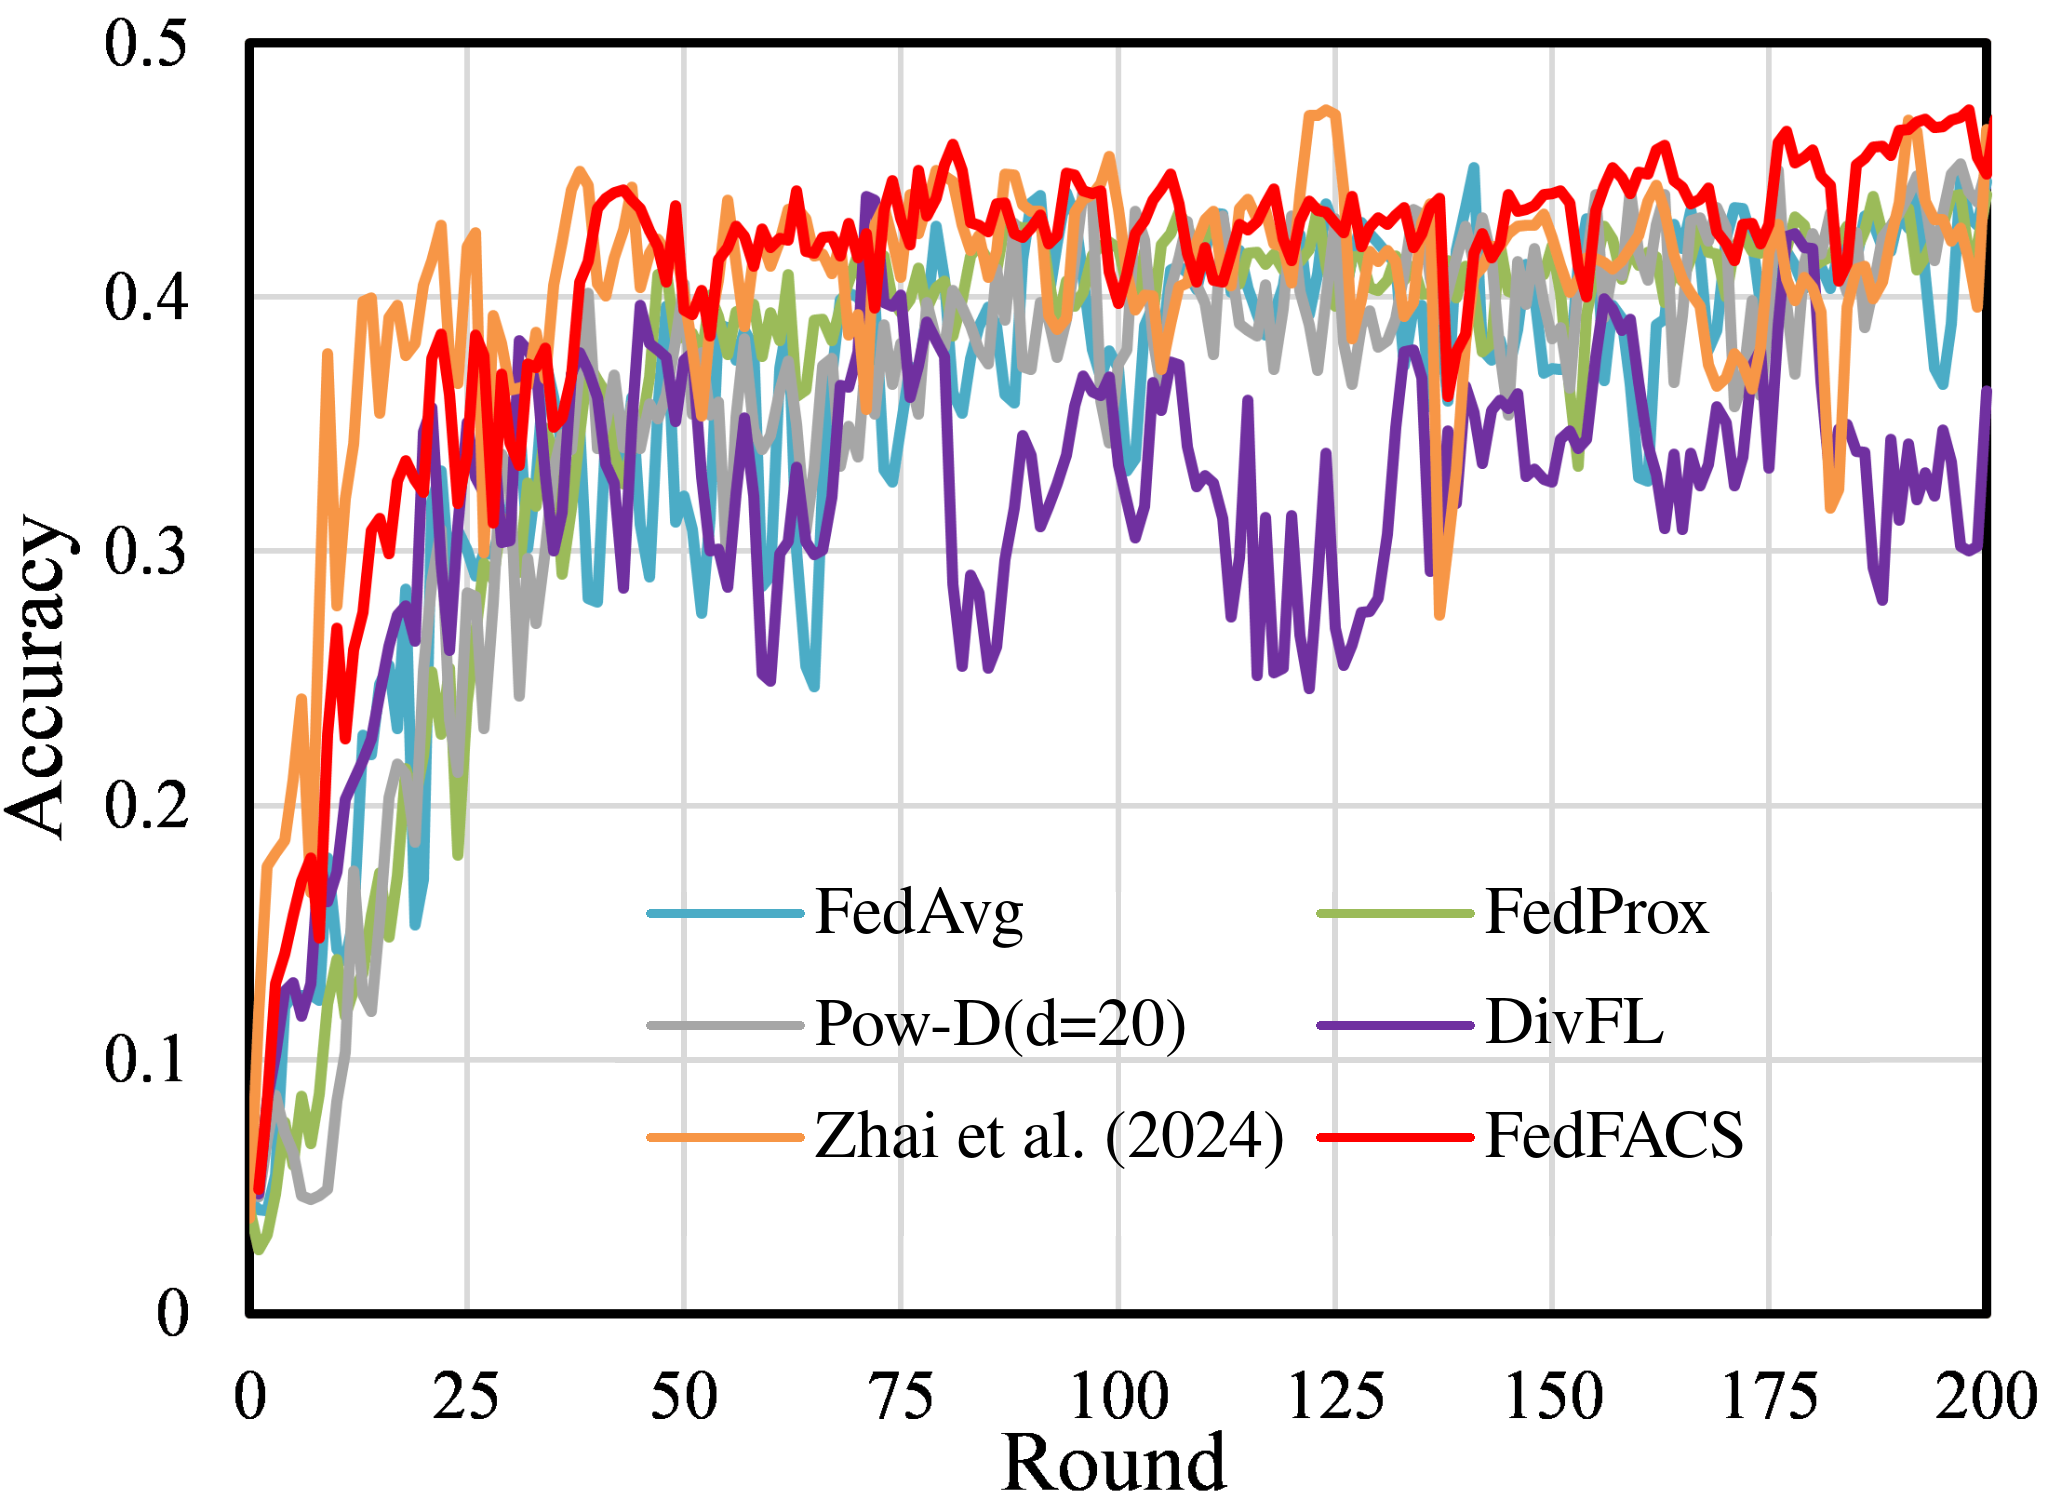
\includegraphics[width=\textwidth]{figs/fig5a.png}\\(a) S1 ($\alpha=0.1$)\end{minipage}\hfill
\begin{minipage}[t]{0.32\textwidth}\centering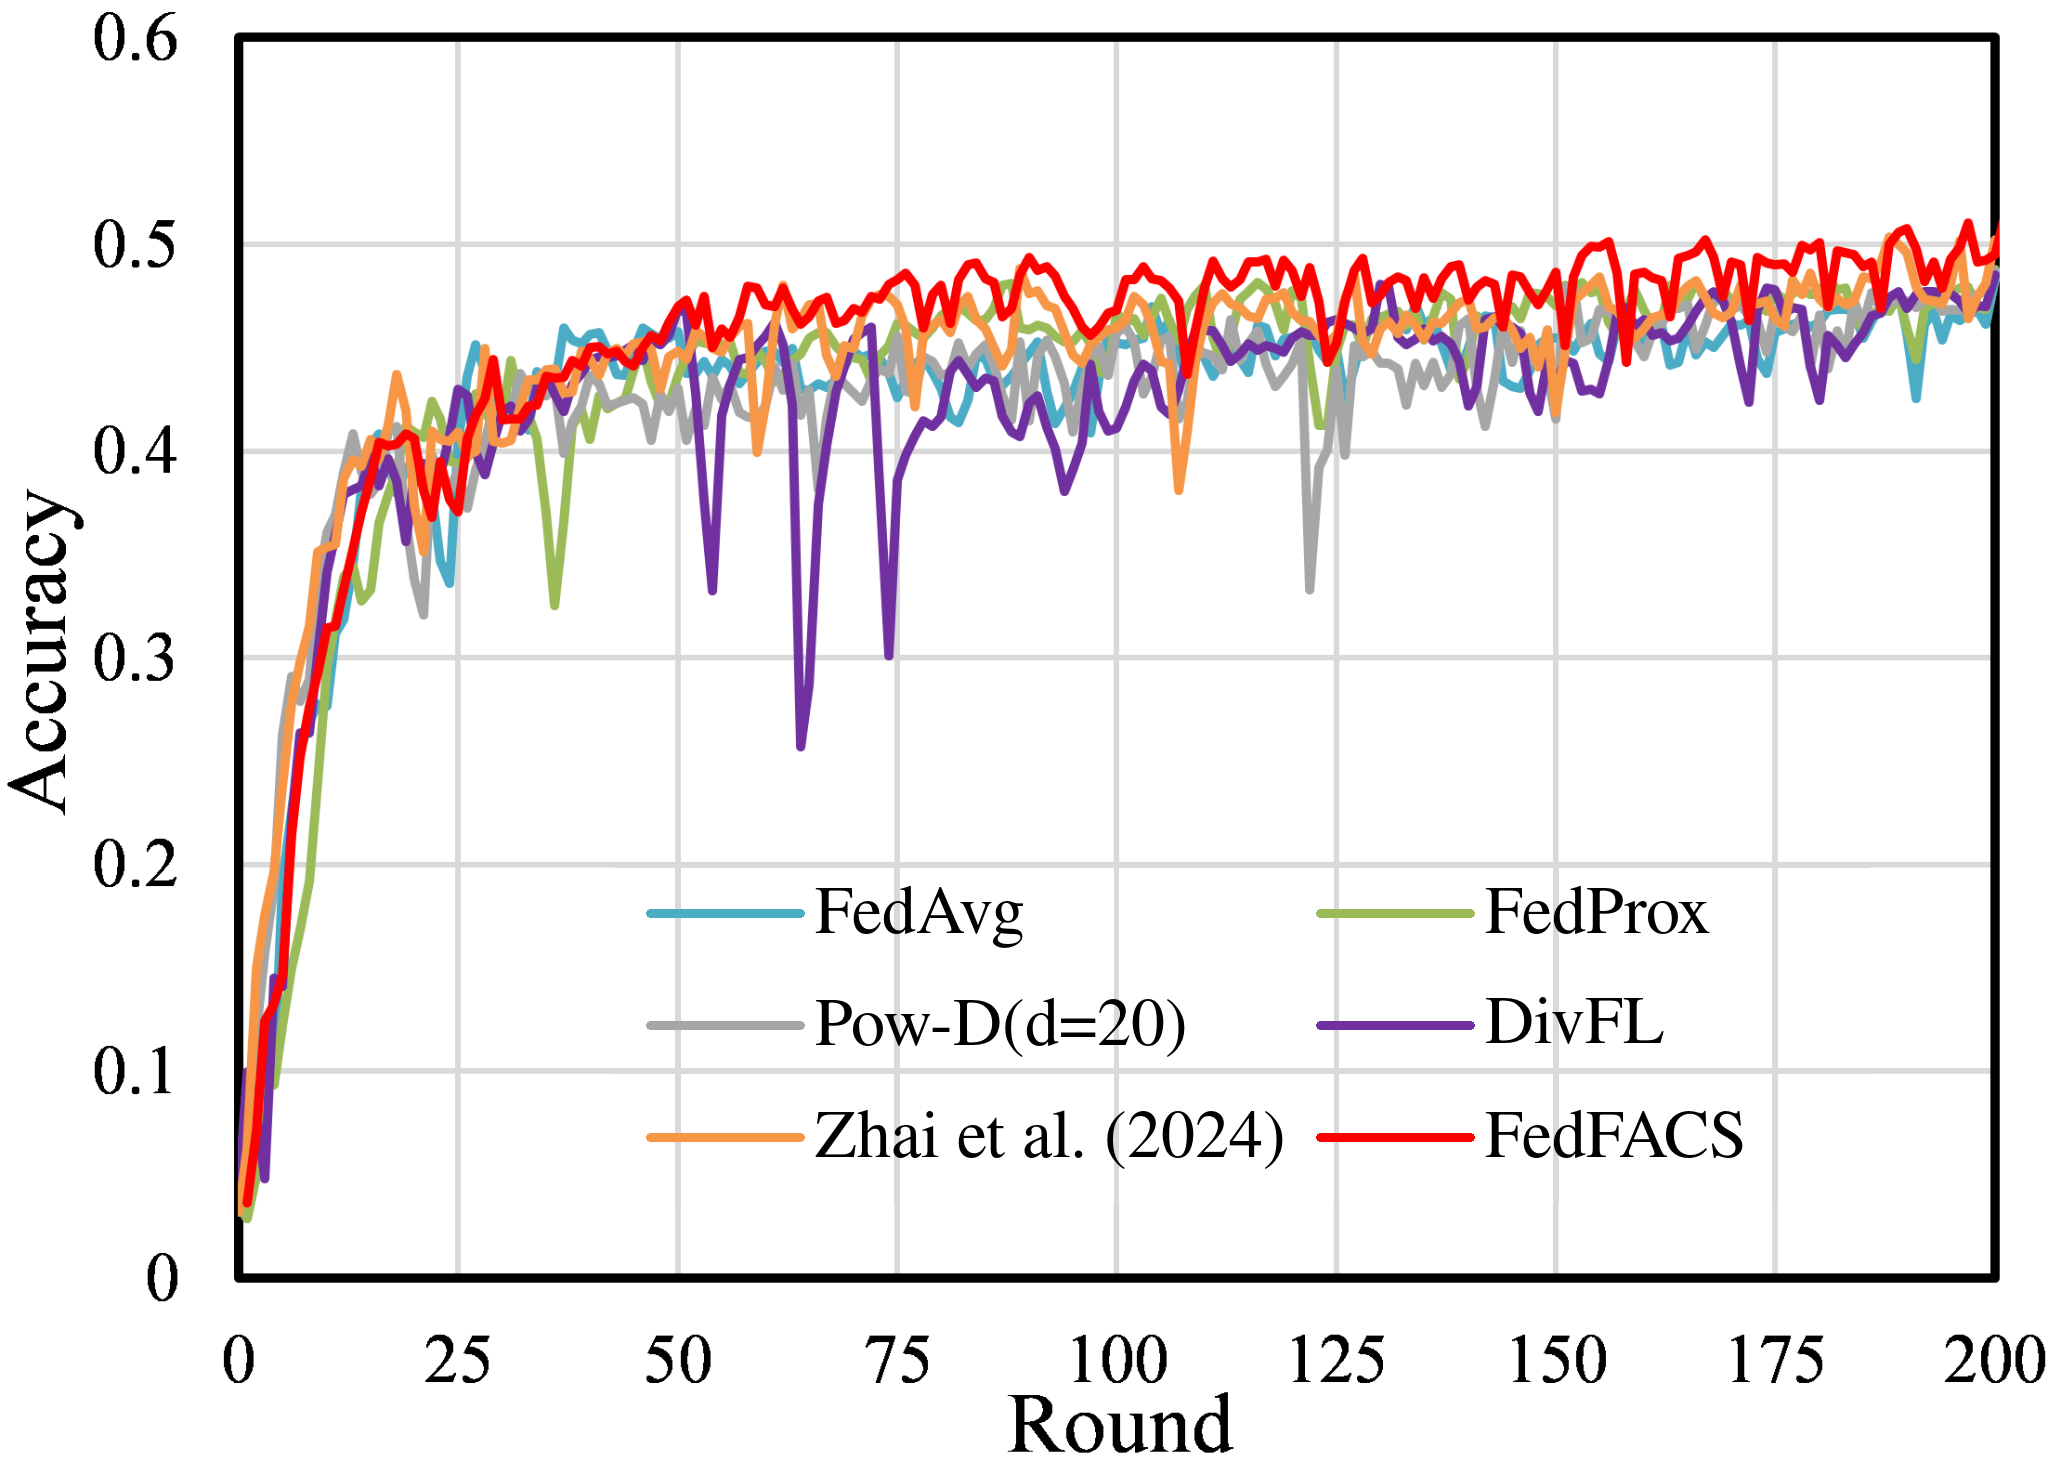
\includegraphics[width=\textwidth]{figs/fig5b.png}\\(b) S1 ($\alpha=0.5$)\end{minipage}\hfill
\begin{minipage}[t]{0.32\textwidth}\centering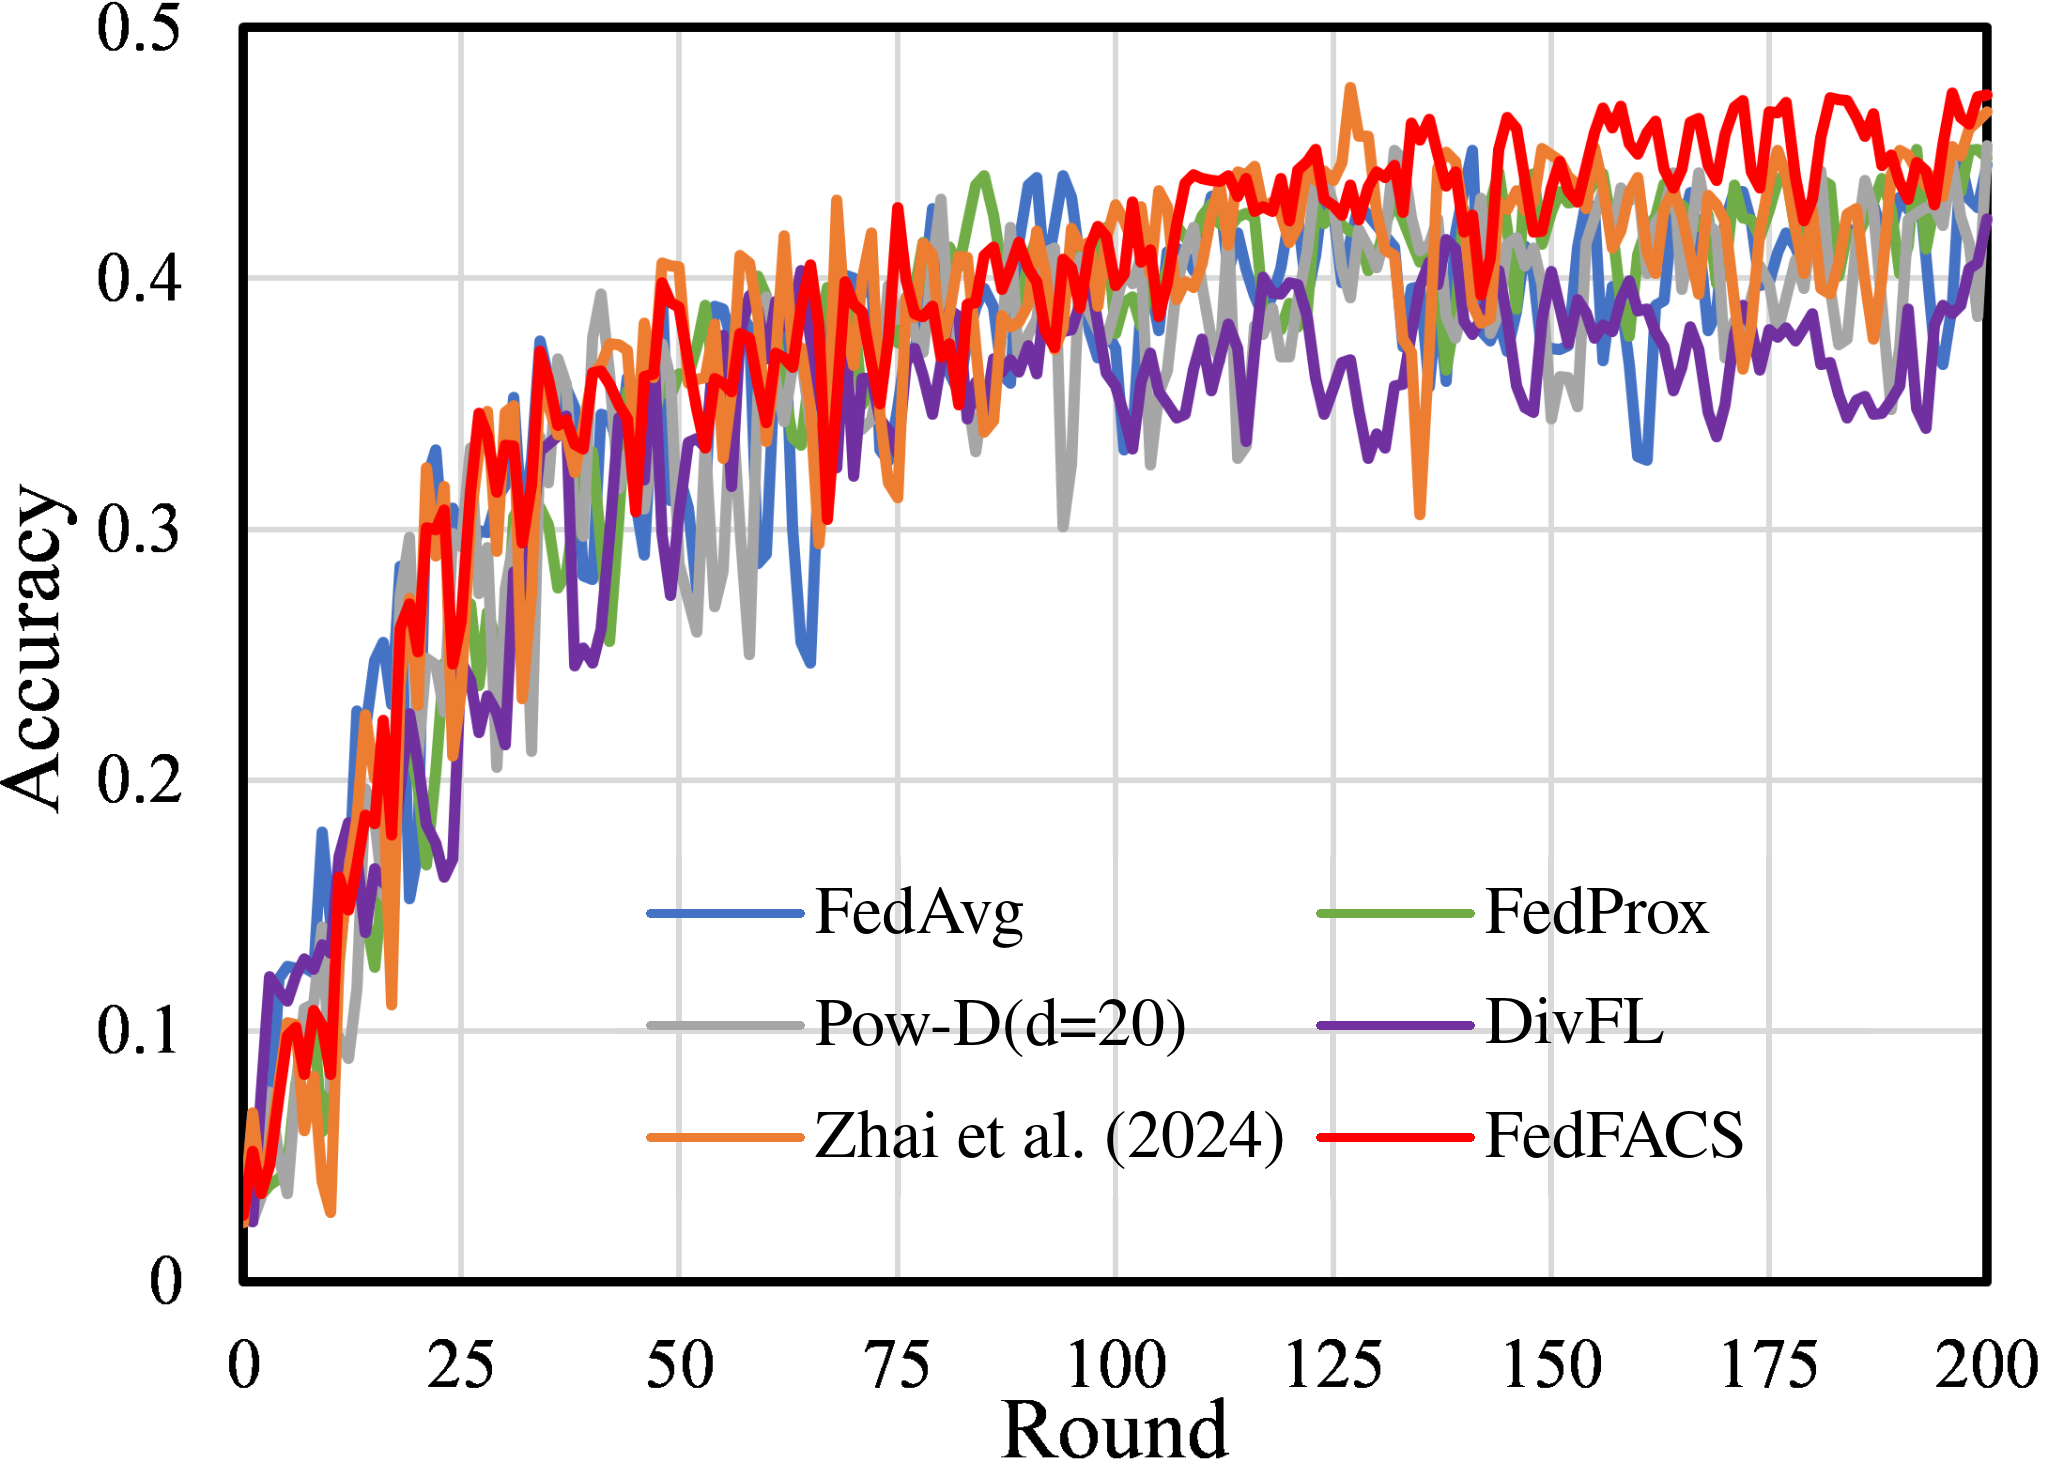
\includegraphics[width=\textwidth]{figs/fig5c.png}\\(c) S2\end{minipage}
\caption{Accuracy under heterogeneous data conditions on CIFAR-10.}\label{fig:cifar}
\end{figure}

\begin{figure}[t]
\centering
\begin{minipage}[t]{0.32\textwidth}\centering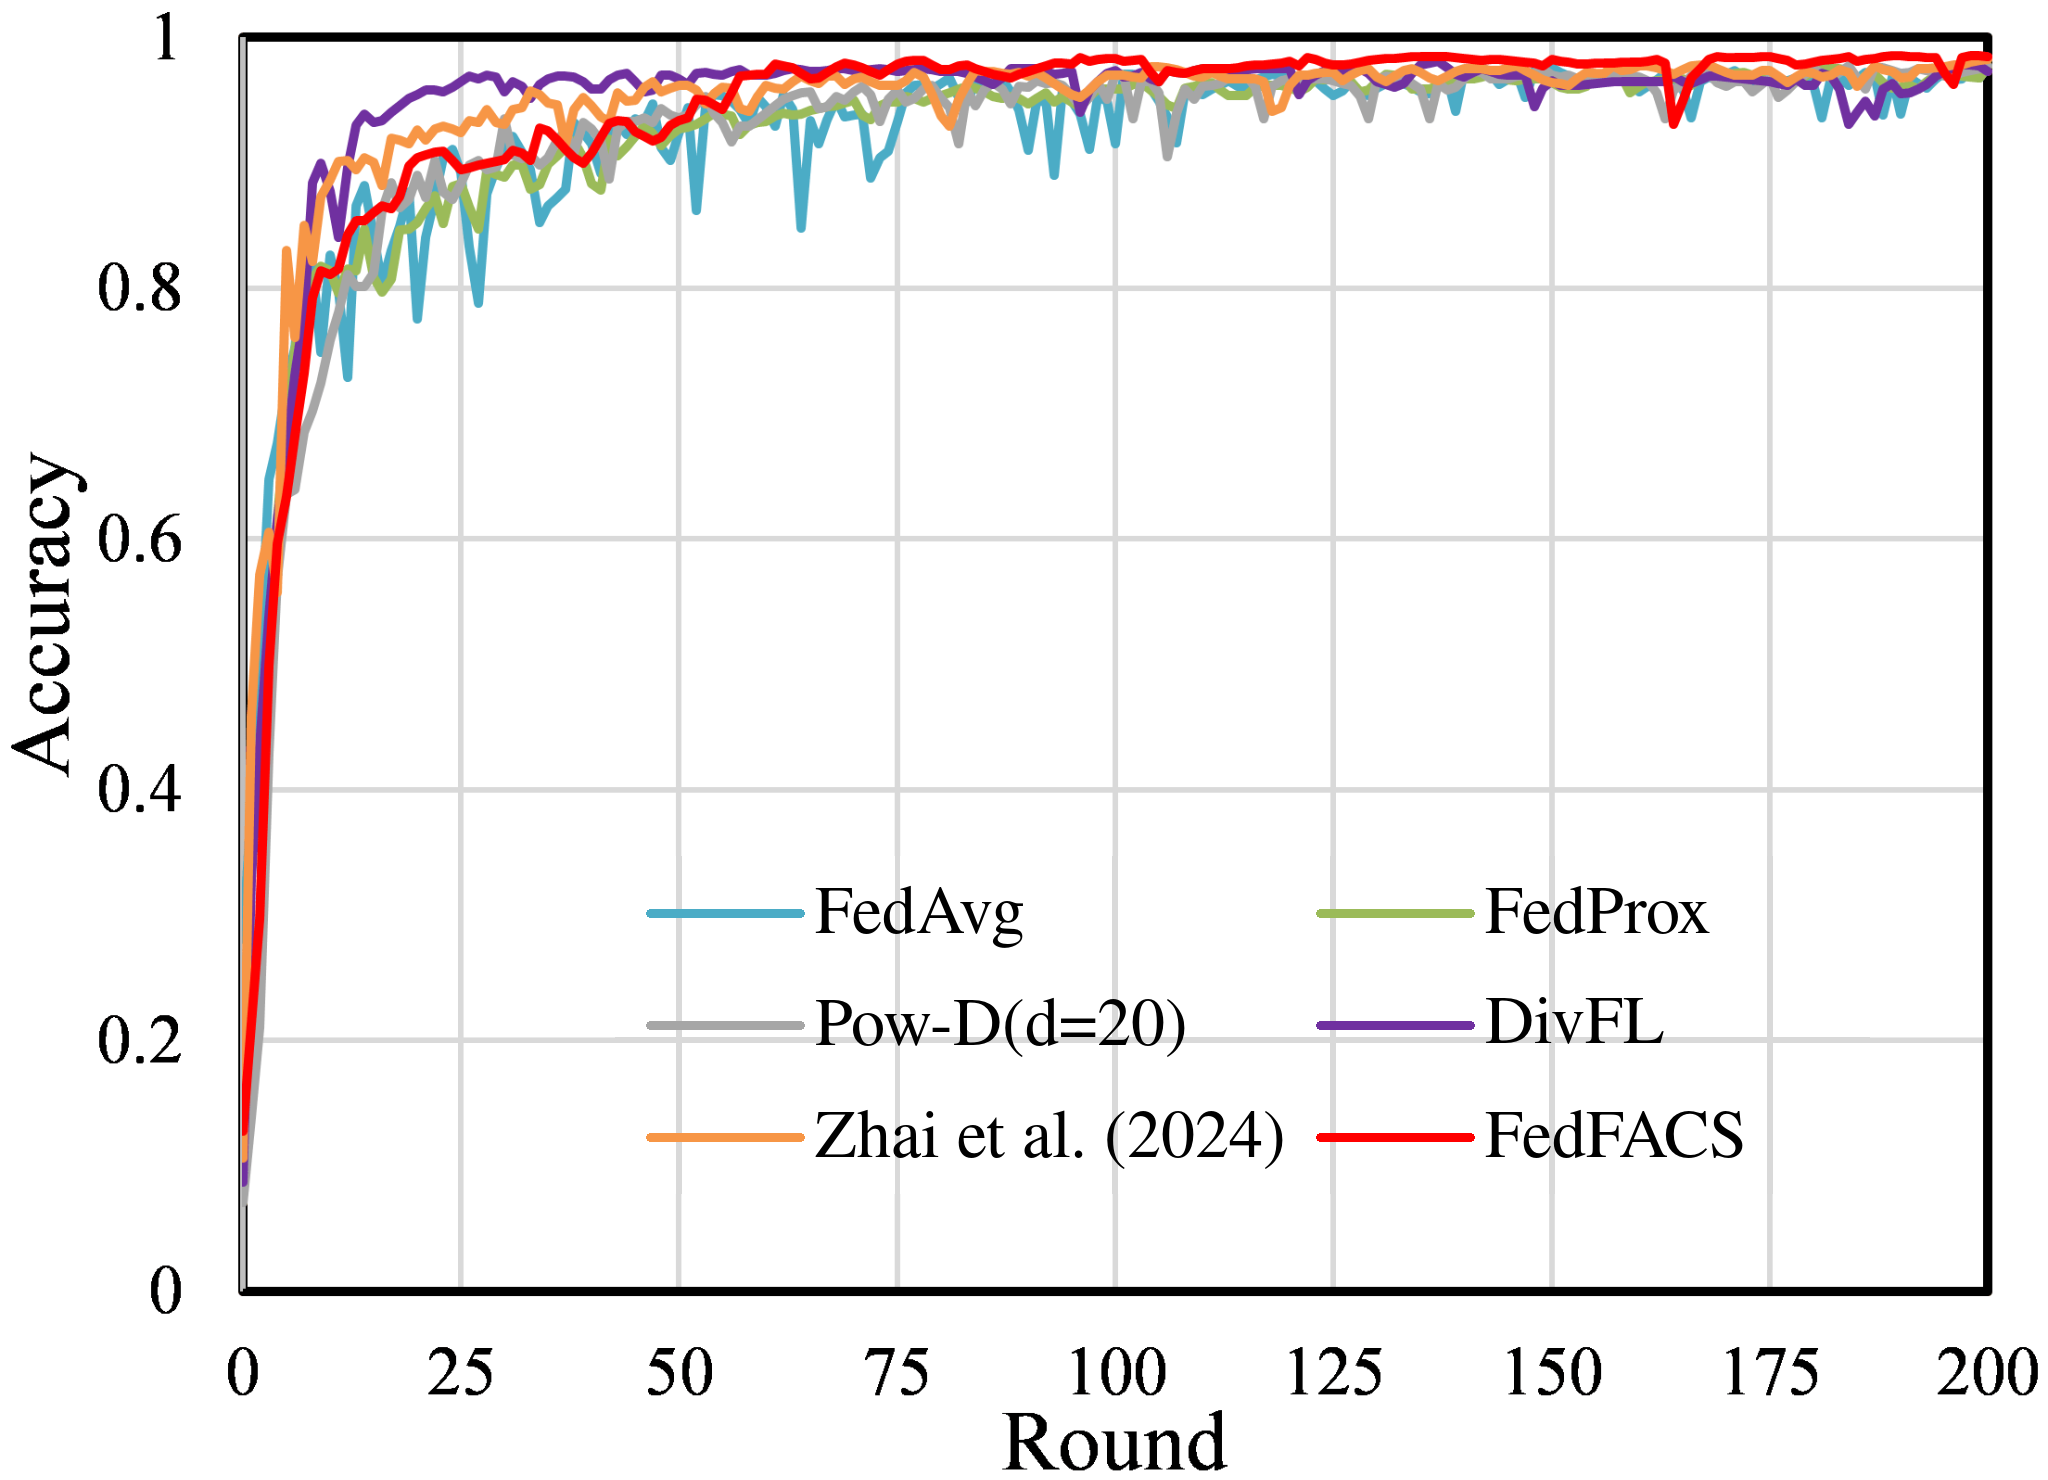
\includegraphics[width=\textwidth]{figs/fig6a.png}\\(a) S1 ($\alpha=0.1$)\end{minipage}\hfill
\begin{minipage}[t]{0.32\textwidth}\centering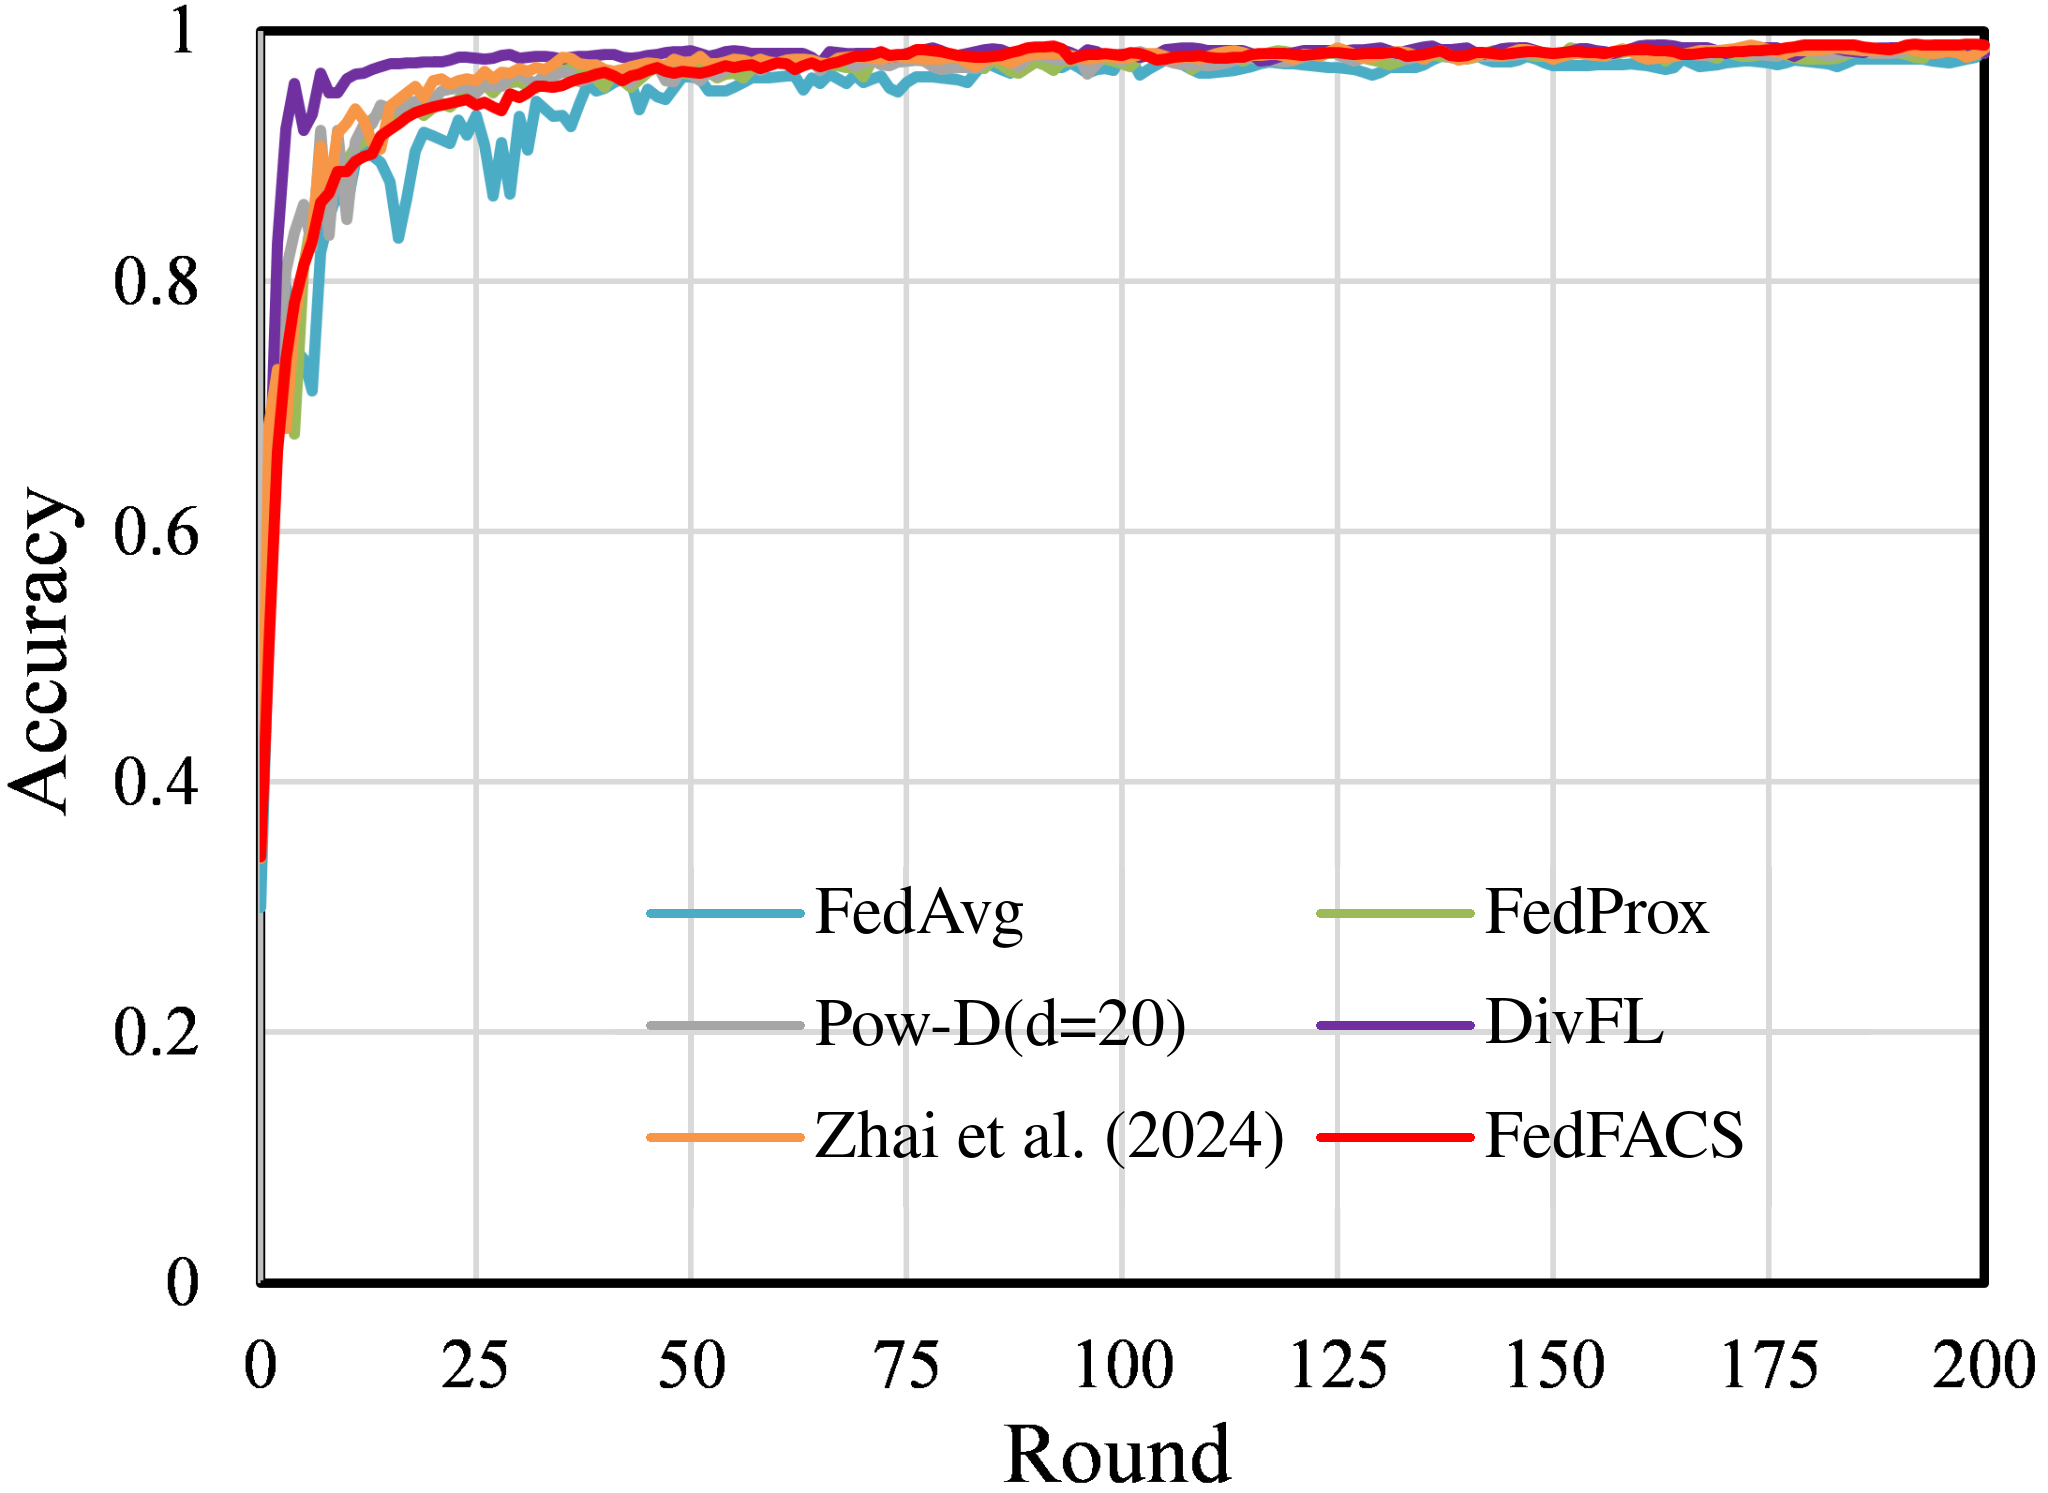
\includegraphics[width=\textwidth]{figs/fig6b.png}\\(b) S1 ($\alpha=0.5$)\end{minipage}\hfill
\begin{minipage}[t]{0.32\textwidth}\centering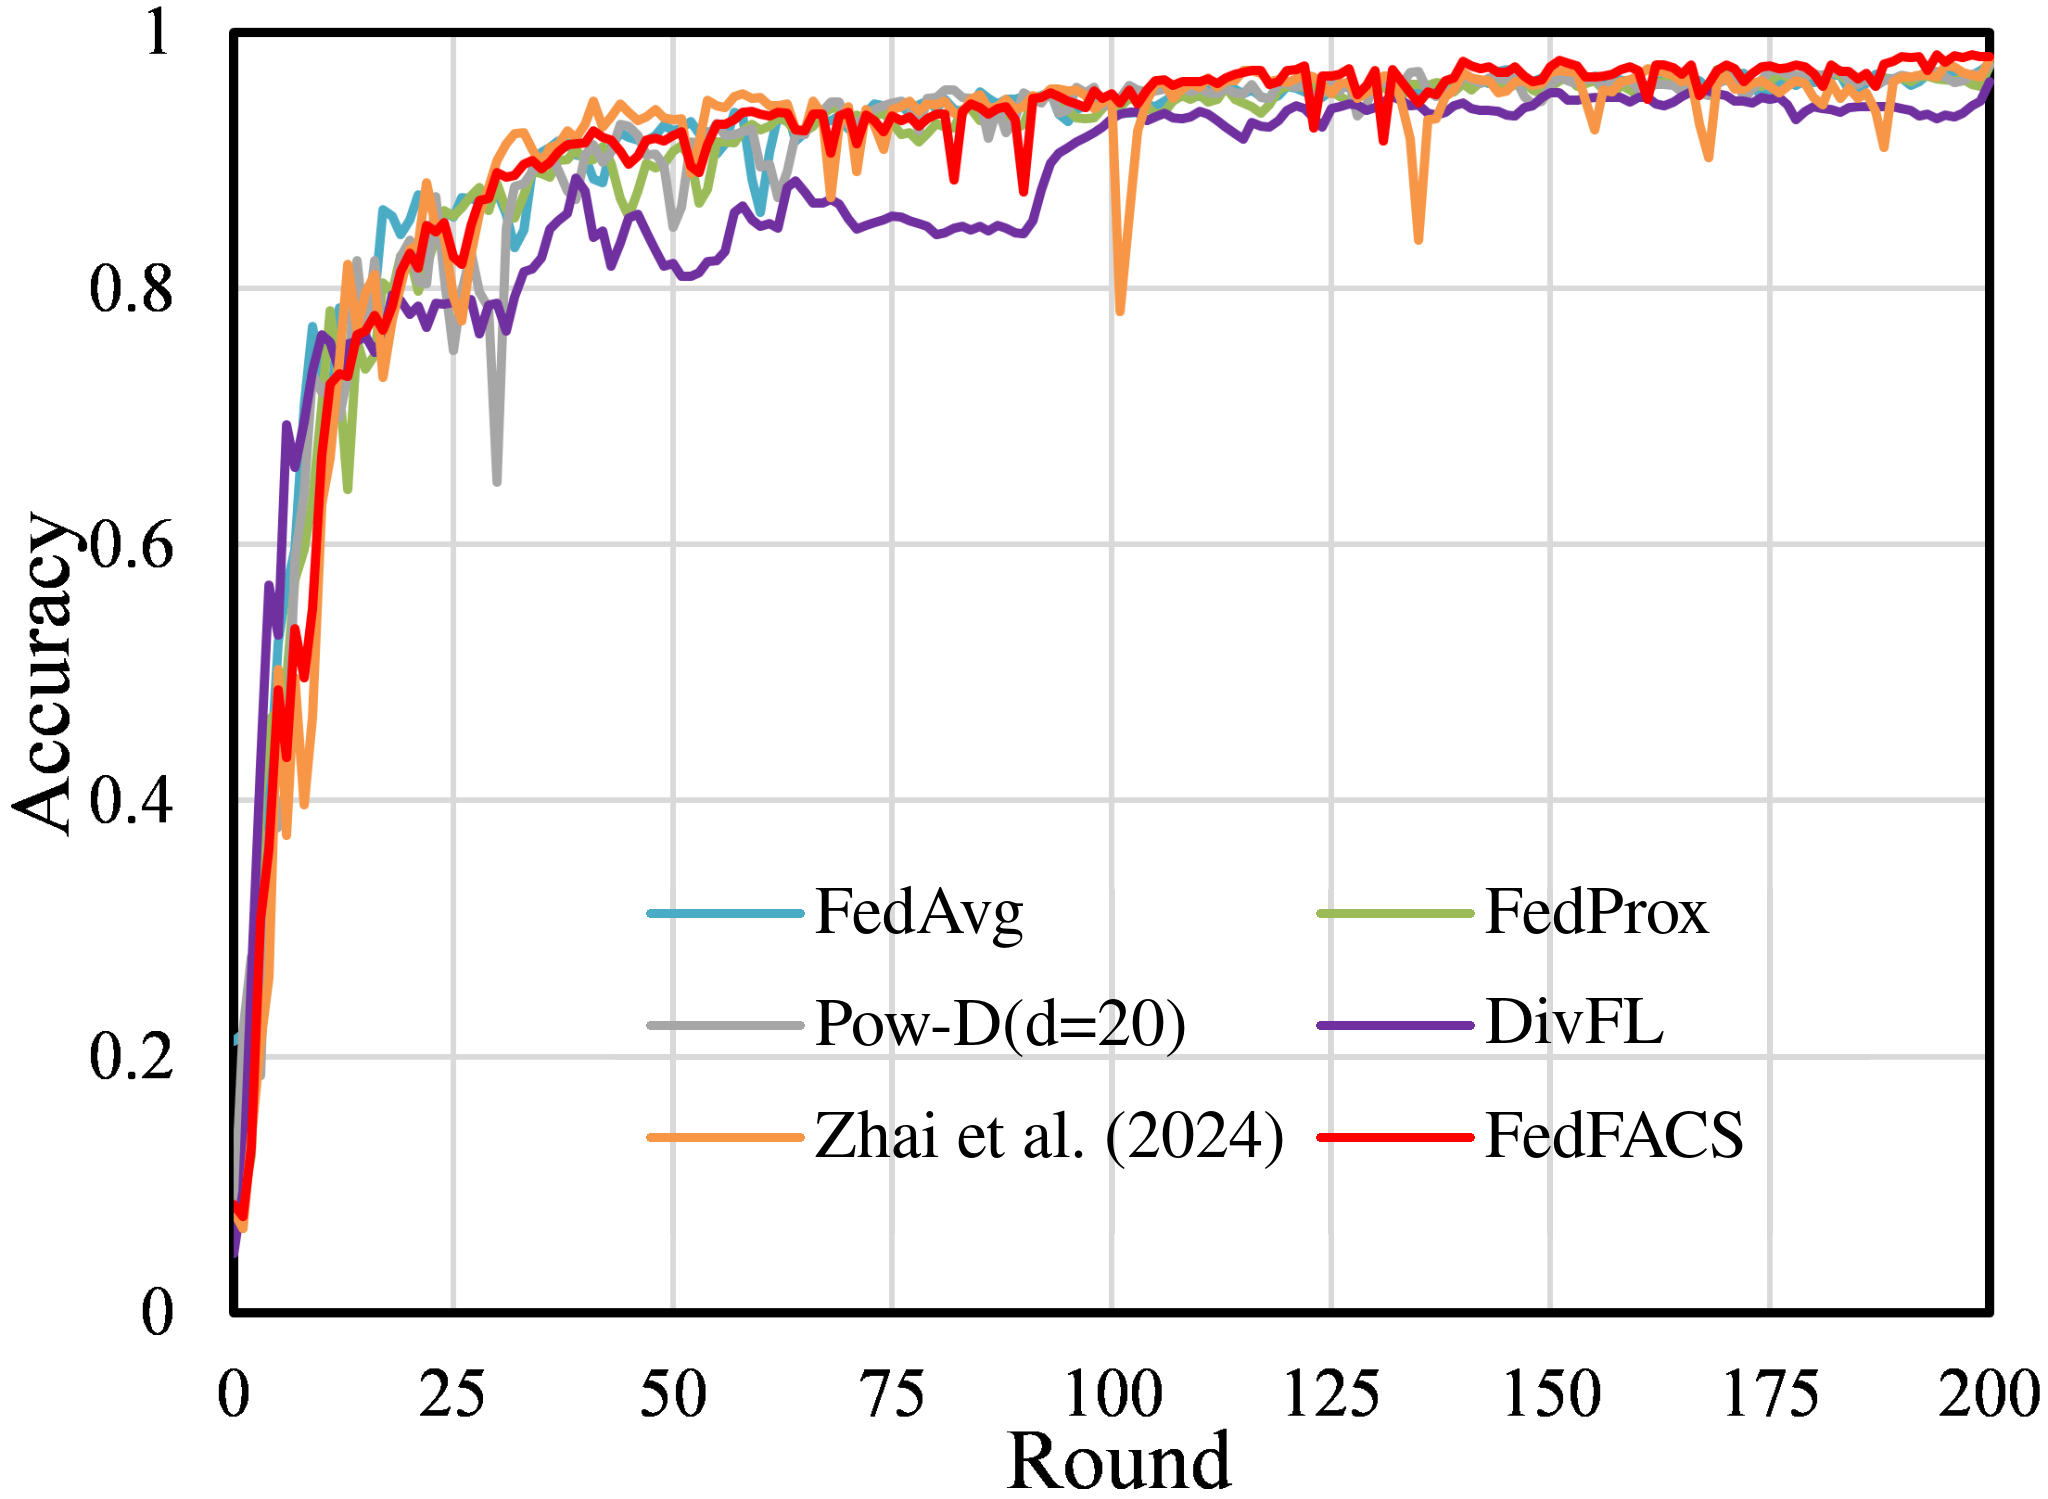
\includegraphics[width=\textwidth]{figs/fig6c.png}\\(c) S2\end{minipage}
\caption{Accuracy under heterogeneous data conditions on MNIST.}\label{fig:mnist}
\end{figure}

\begin{figure}[t]
\centering
\begin{minipage}[t]{0.32\textwidth}\centering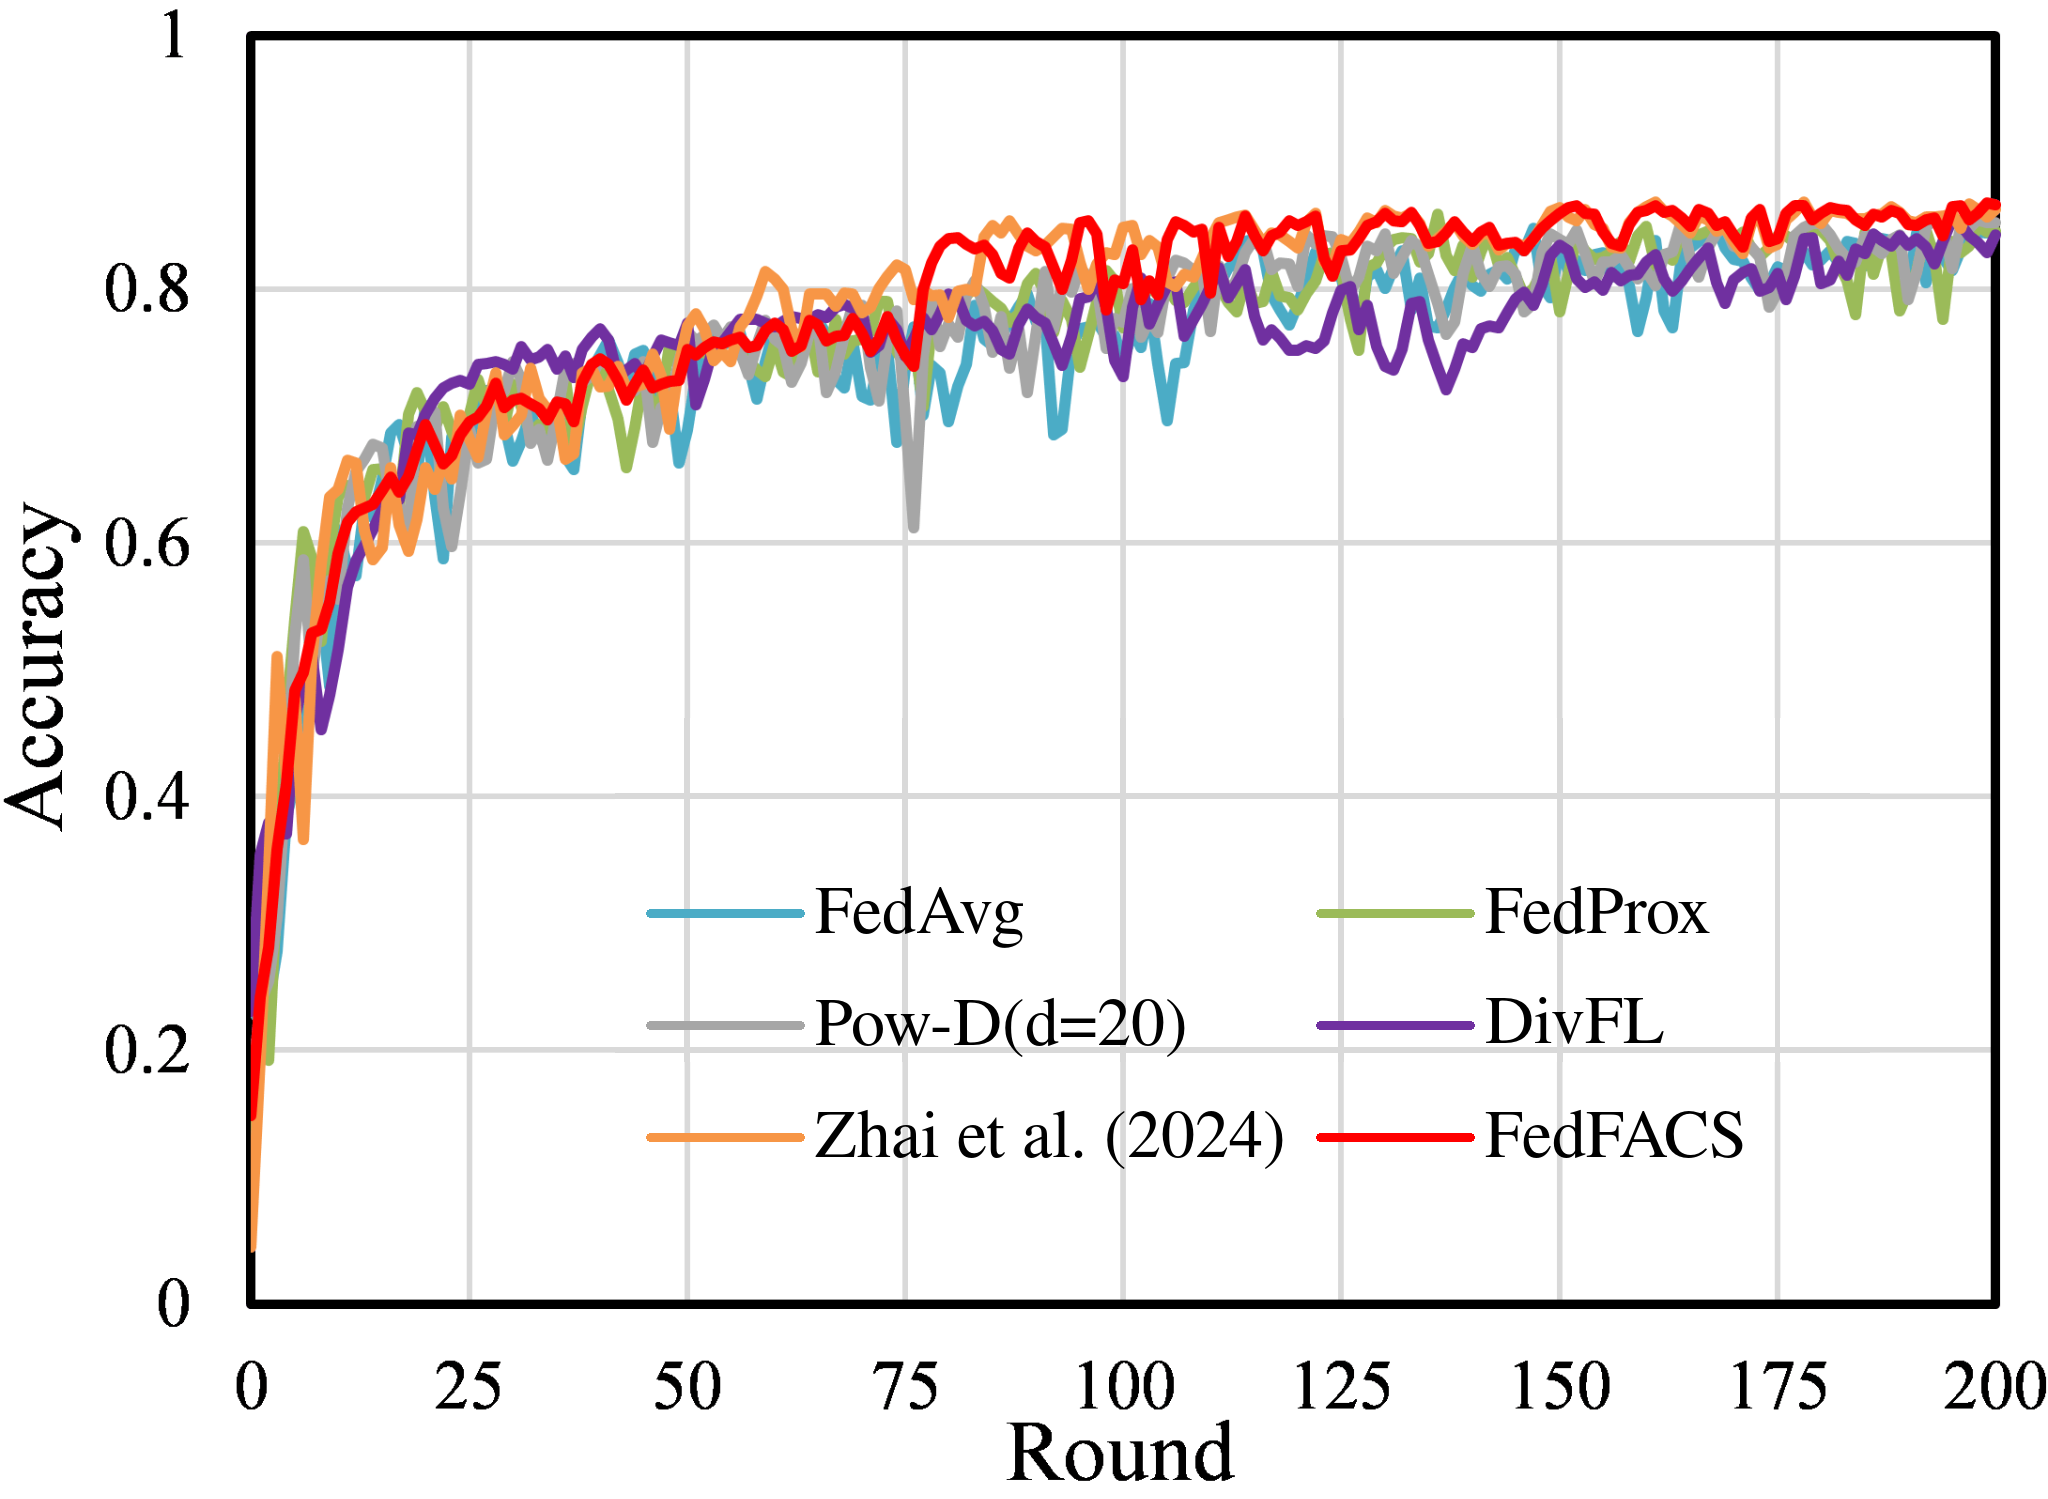
\includegraphics[width=\textwidth]{figs/fig7a.png}\\(a) S1 ($\alpha=0.1$)\end{minipage}\hfill
\begin{minipage}[t]{0.32\textwidth}\centering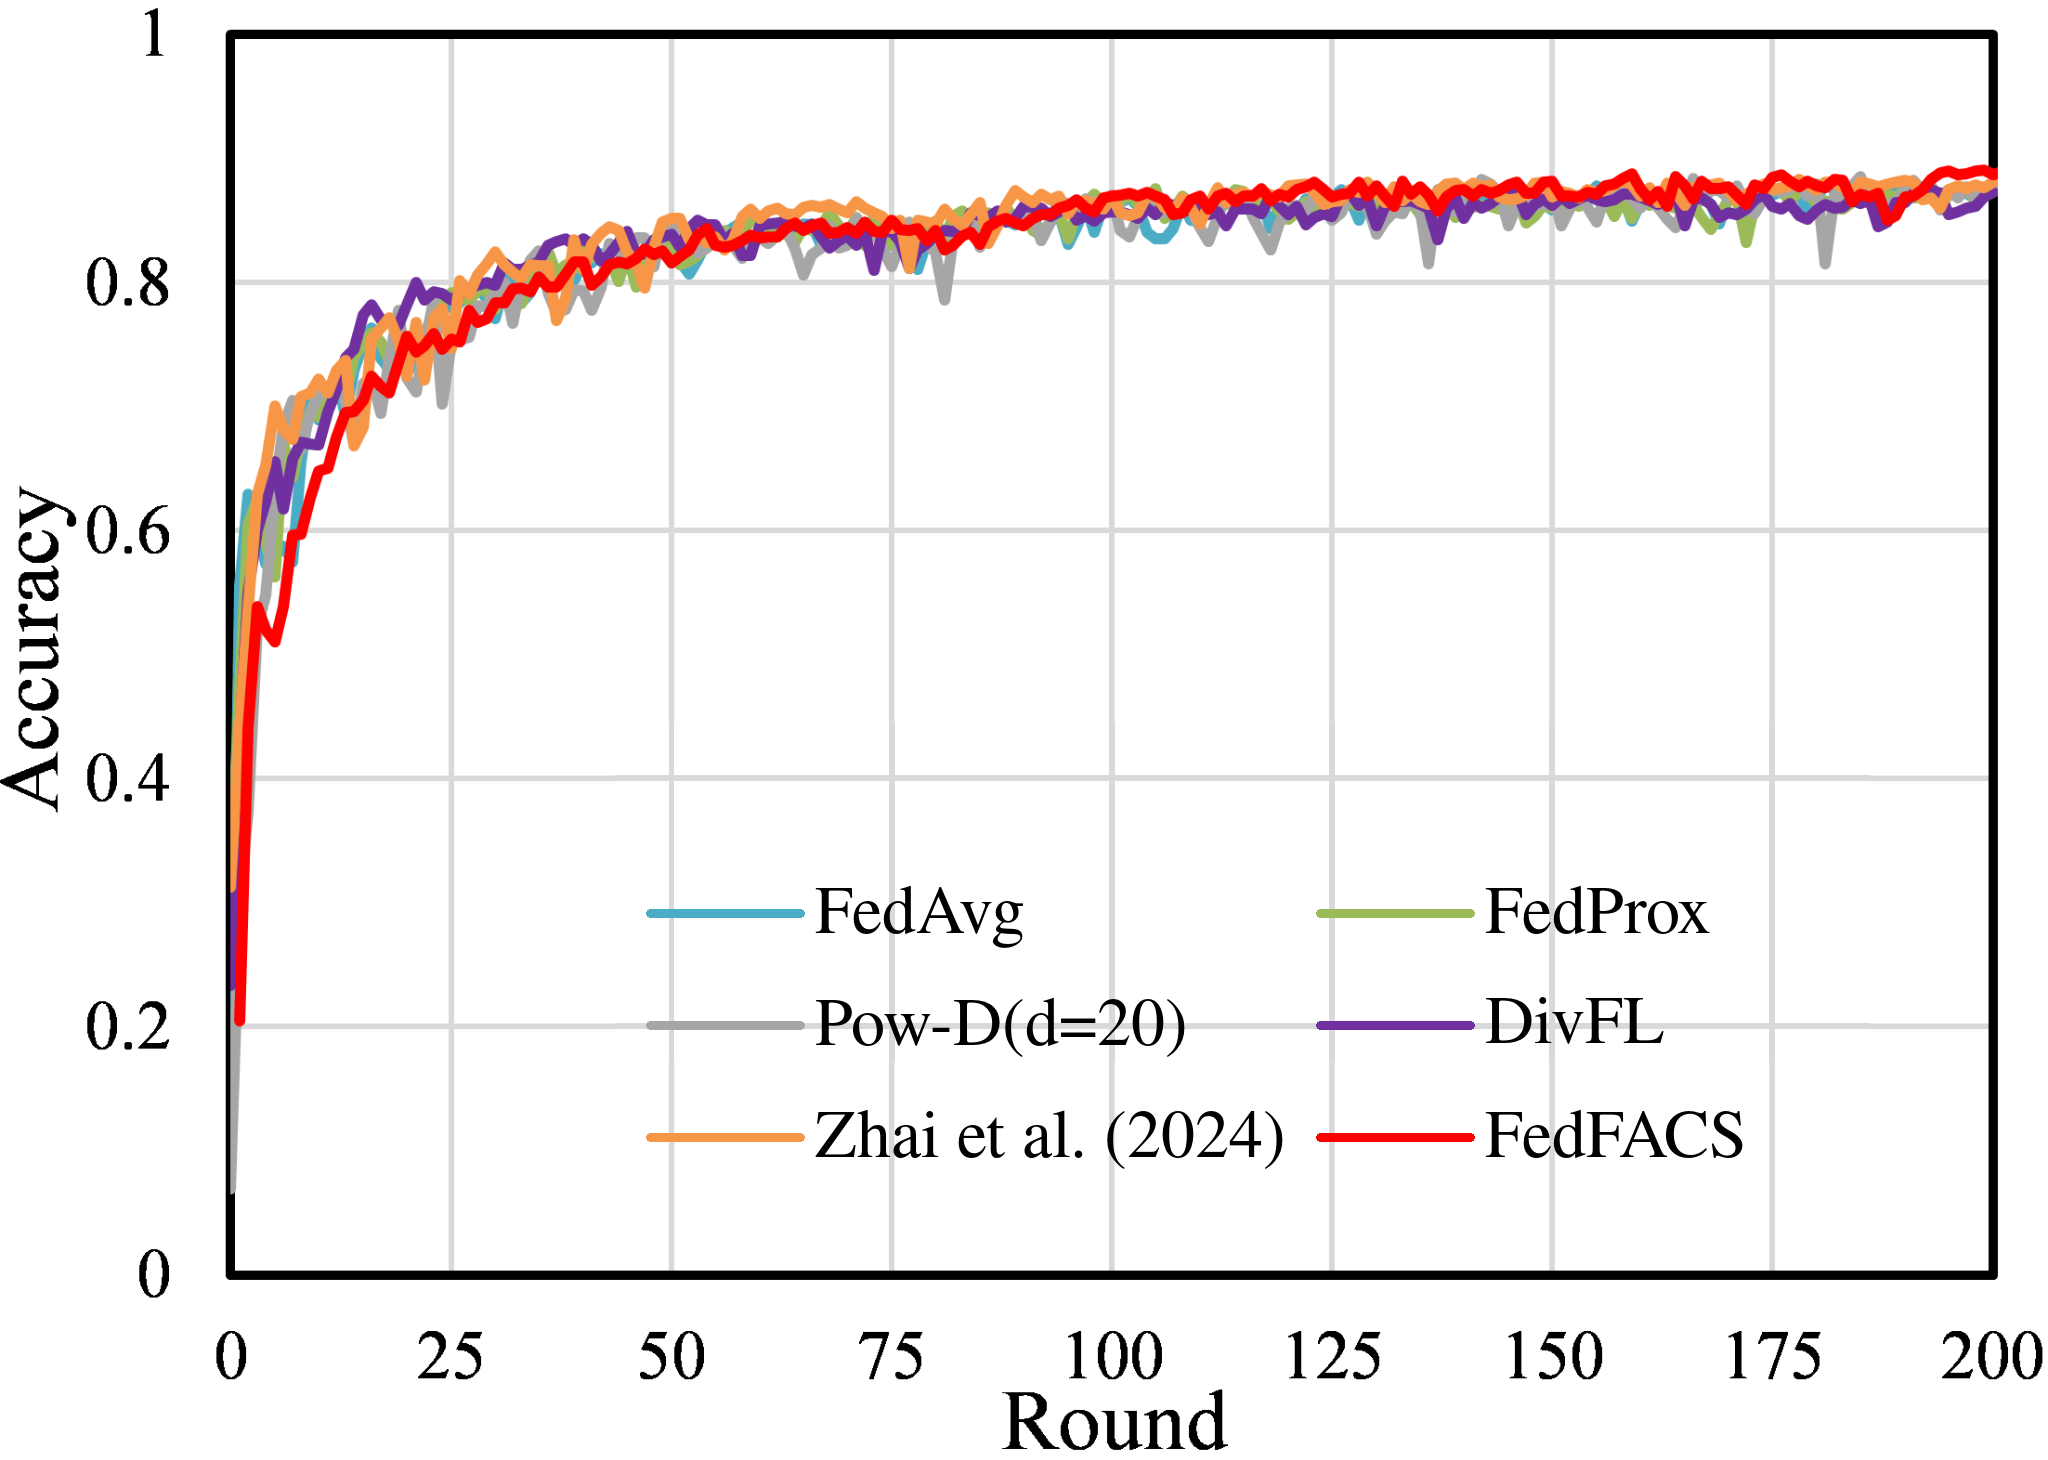
\includegraphics[width=\textwidth]{figs/fig7b.png}\\(b) S1 ($\alpha=0.5$)\end{minipage}\hfill
\begin{minipage}[t]{0.32\textwidth}\centering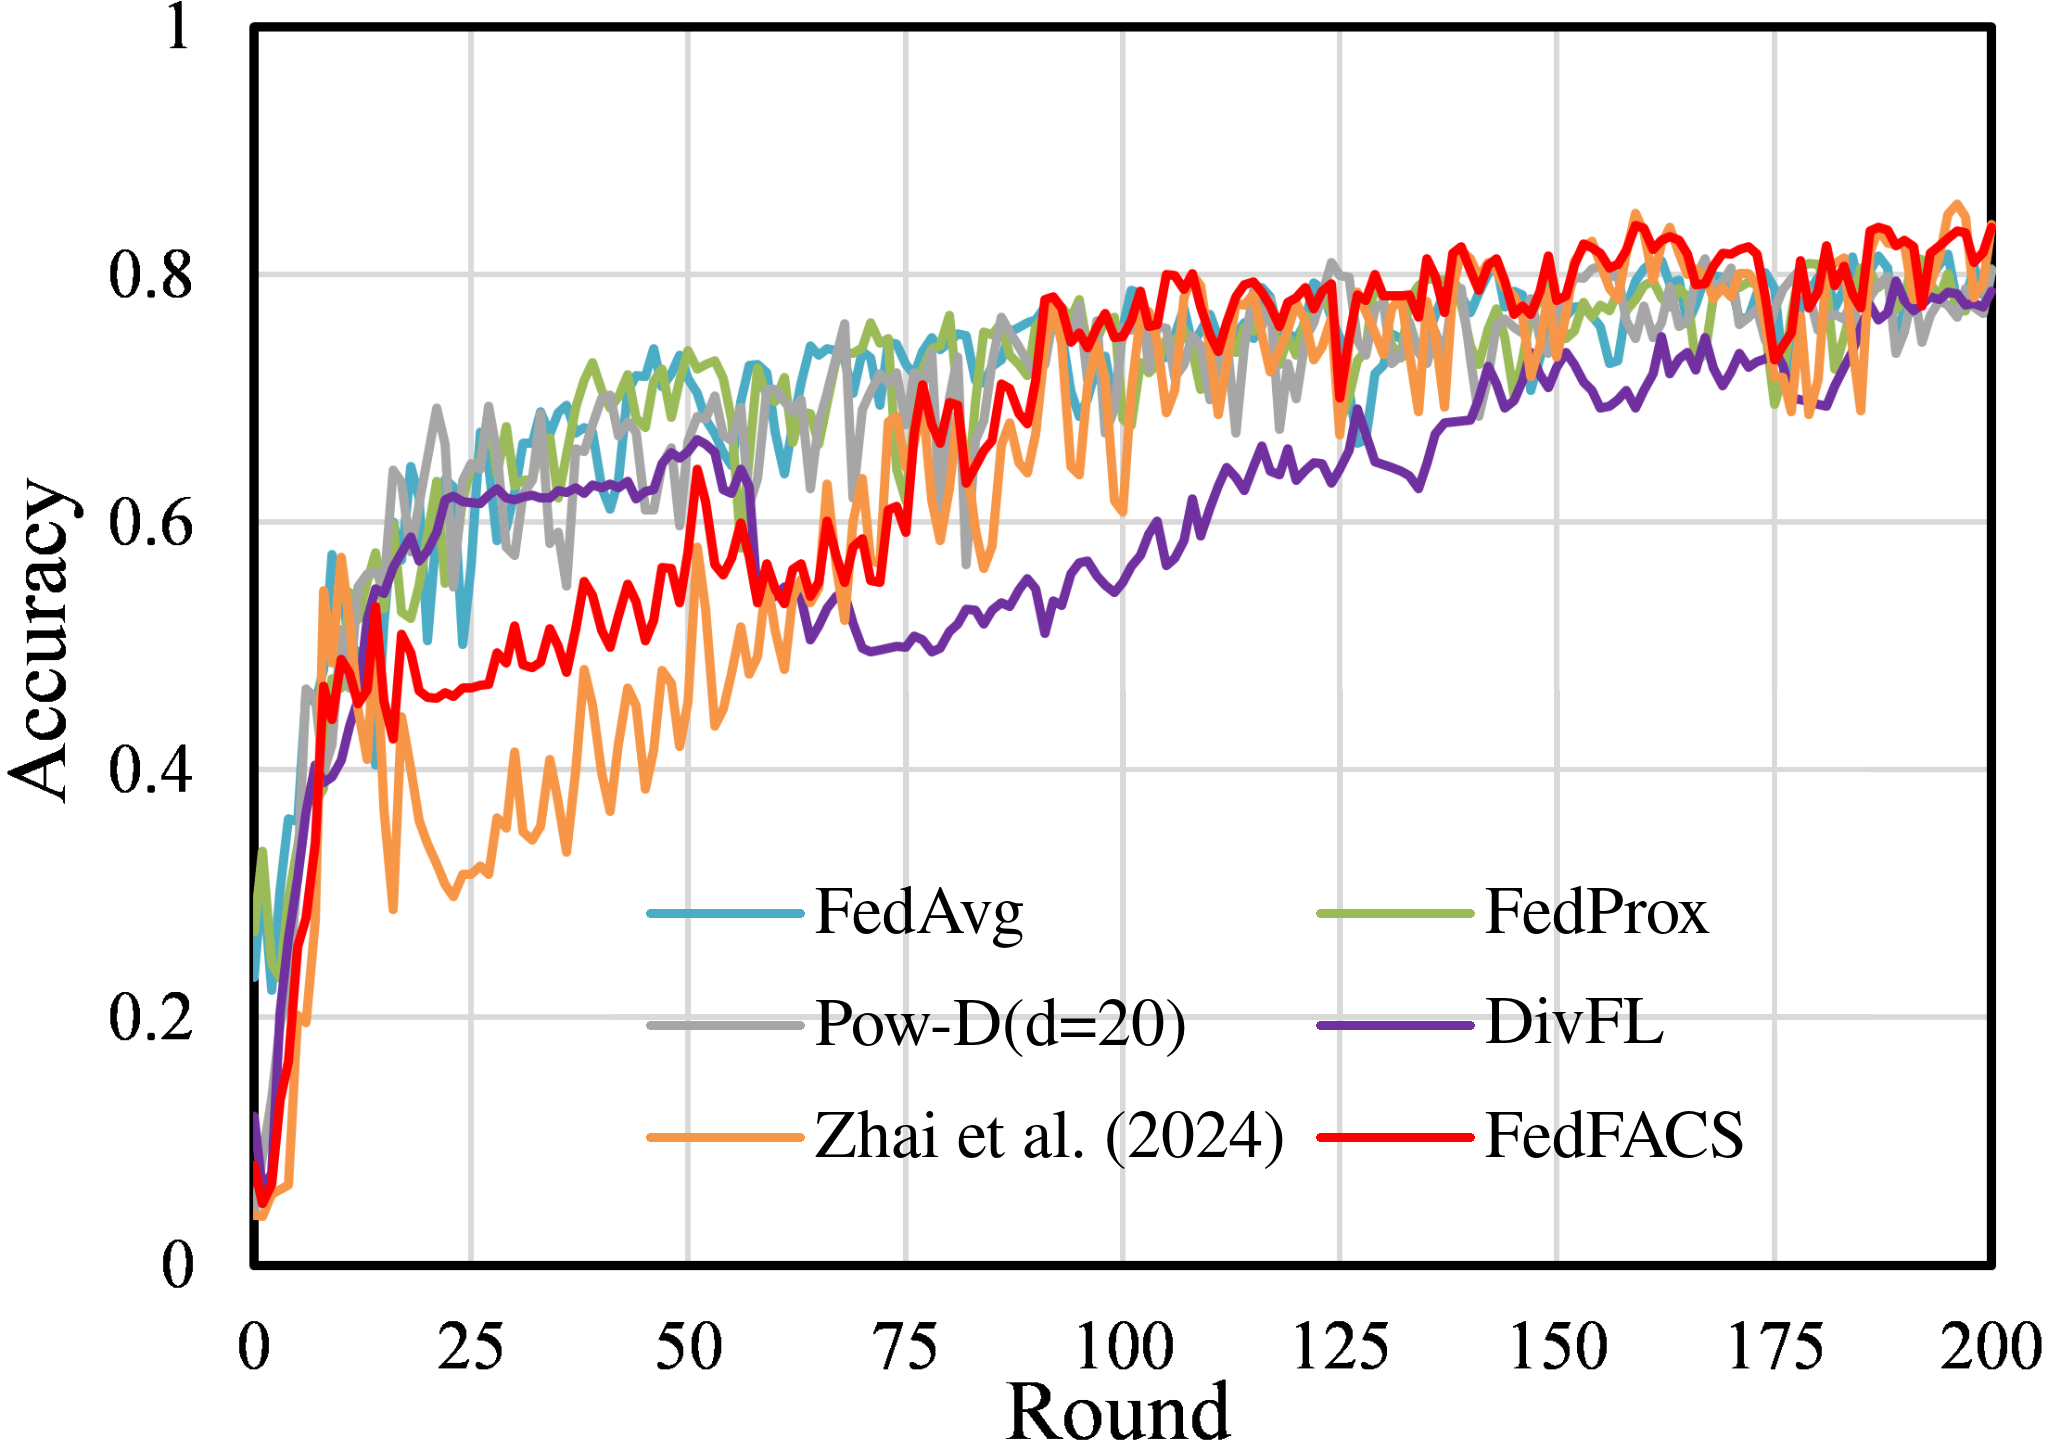
\includegraphics[width=\textwidth]{figs/fig7c.png}\\(c) S2\end{minipage}
\caption{Accuracy under heterogeneous data conditions on FMNIST.}\label{fig:fmnist}
\end{figure}

\subsubsection{Configuration B: comparison with Random, Pow-D and AHIBCS}
FedFACS reaches accuracies of 87.1\%, 54.3\% and 95.3\% on FMNIST, CIFAR-10 and COVID-19, against 85.9\%, 53.1\% and 94.8\% for AHIBCS (Fig.~\ref{fig:cfgB}). The absolute gains are 1.2, 1.2 and 0.5 percentage points (pp), equivalent to relative gains of 1.40\%, 2.26\% and 0.53\%. Over the other two methods the accuracy of FedFACS is higher by 5.5 pp (Random) and 3.6 pp (Pow-D) on FMNIST, 3.0 pp and 5.3 pp on CIFAR-10 and 3.6 pp and 2.2 pp on COVID-19. At accuracy targets of 83\%, 50\% and 91\%, FedFACS requires 35, 151 and 103 rounds against 27, 144 and 110 for AHIBCS (Table~\ref{tab:cfgB}). Cumulative uploads are 266, 1{,}381 and 1{,}047 against 270, 1{,}440 and 1{,}100, that is 1.5\%, 4.1\% and 4.8\% fewer. FedFACS therefore uploads less in all three cases but needs 29.6\% more rounds on FMNIST and 4.9\% more on CIFAR-10; only on COVID-19 (6.4\% fewer rounds) does it also converge faster. A small reduction in uploads on FMNIST thus comes with a substantial increase in rounds. On COVID-19 recall is 0.934 against 0.948 for AHIBCS, while F1 is 0.950 against 0.945 (Table~\ref{tab:prf}). Mean cohort sizes (uploads per round) are 7.6, 9.1 and 10.2 for FedFACS on FMNIST, CIFAR-10 and COVID-19. A mean of 7.6 requires at least one round with fewer than 8 clients and a mean of 10.2 requires at least one round with more than 10, so Configuration~B must have used bounds different from the $(8,10)$ of the Configuration~A ablation; the actual bounds and the per-round cohort sizes were not recorded. The fewer-uploads result must also be separated from the effect of reaching a target in fewer rounds: on COVID-19 both contribute, whereas on FMNIST and CIFAR-10 the saving comes from smaller per-round cohorts despite more rounds. Fig.~\ref{fig:gain} labels the gains between adjacent methods in absolute percentage points.

\begin{figure}[t]
\centering
\begin{minipage}[t]{0.48\textwidth}\centering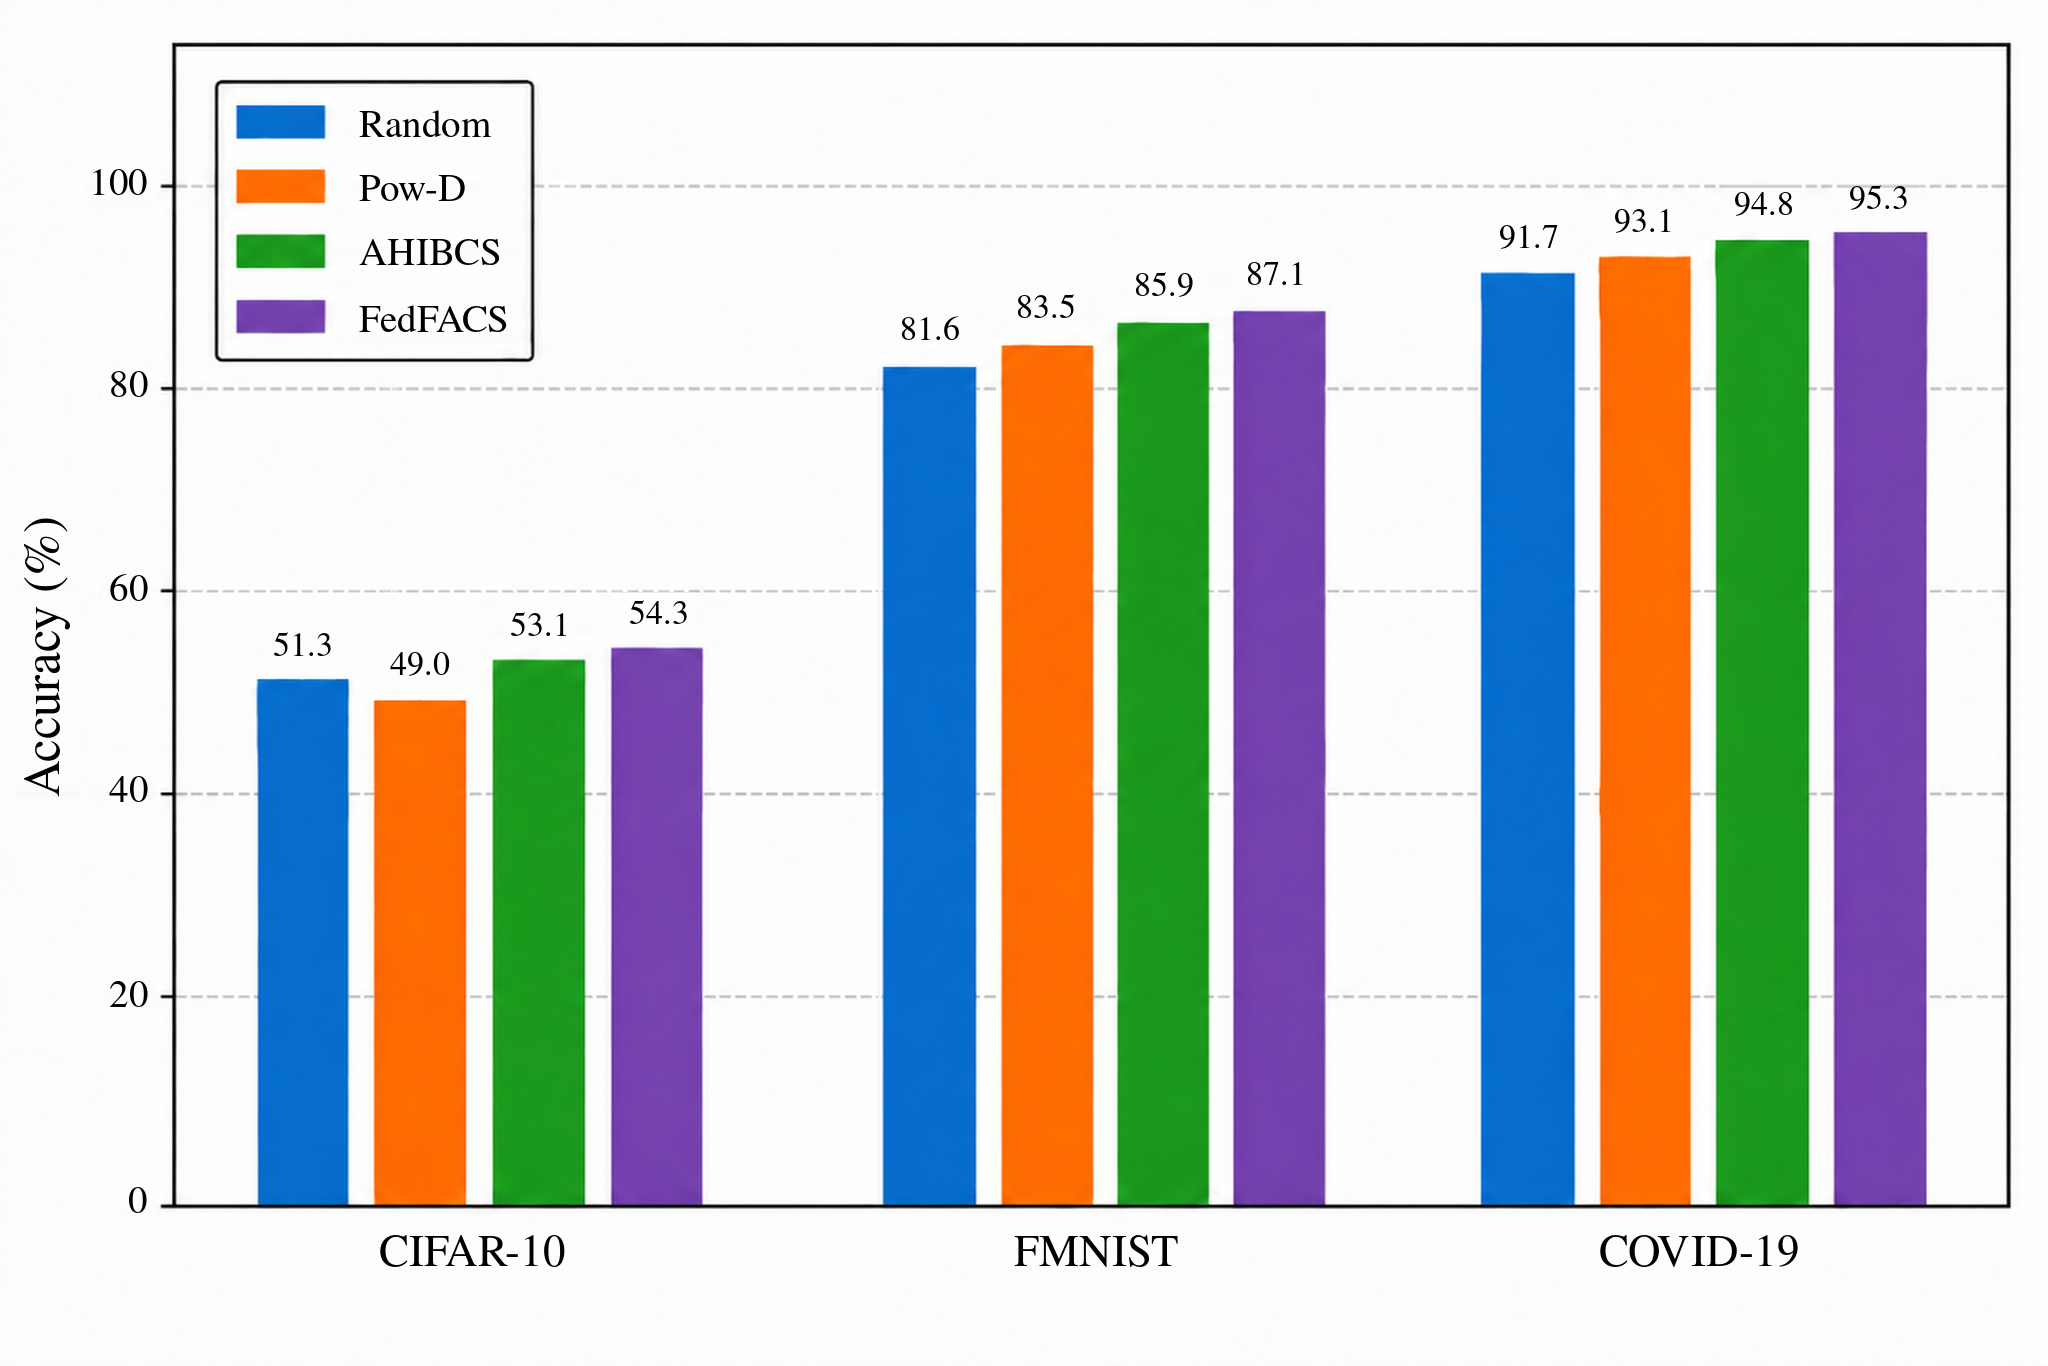
\includegraphics[width=\textwidth]{figs/fig8.png}\caption{Accuracy of Random, Pow-D, AHIBCS and FedFACS (Configuration~B).}\label{fig:cfgB}\end{minipage}\hfill
\begin{minipage}[t]{0.48\textwidth}\centering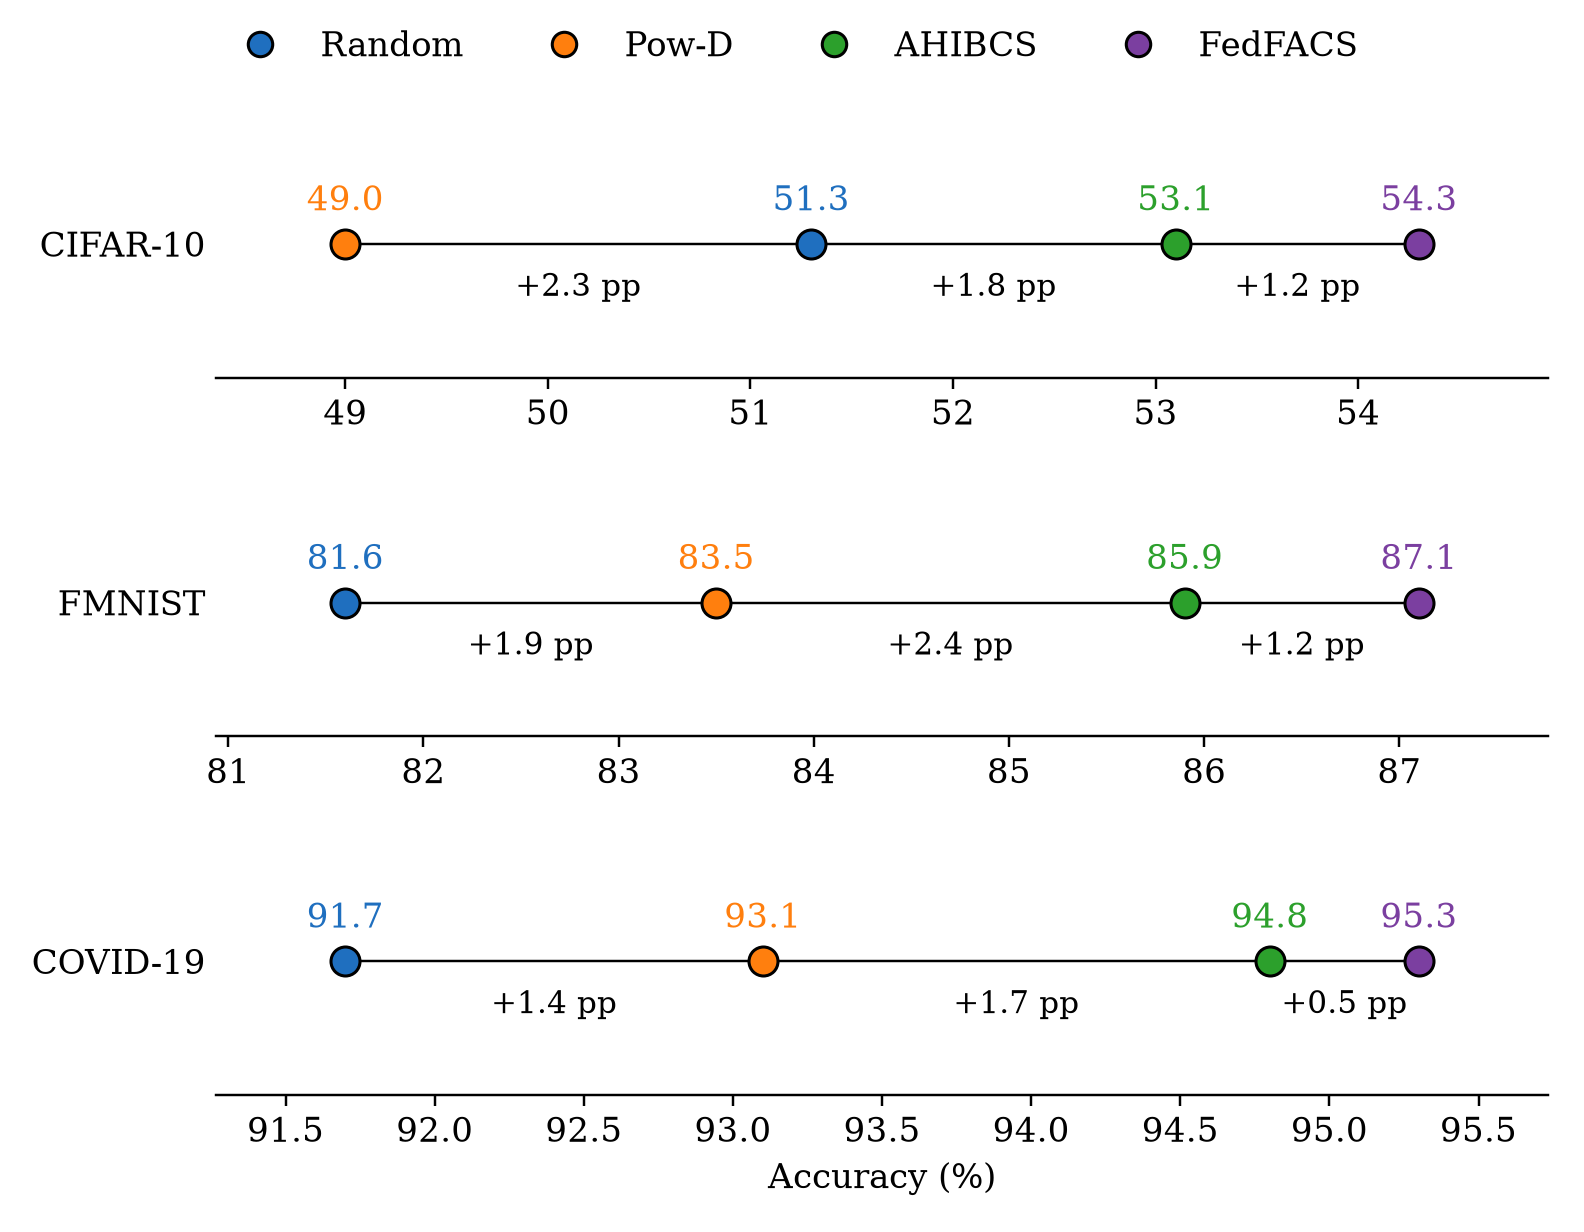
\includegraphics[width=\textwidth]{figs/fig9_corrected.png}\caption{Accuracy and gain between adjacent methods in percentage points (pp), from the values of Fig.~\ref{fig:cfgB}.}\label{fig:gain}\end{minipage}
\end{figure}

\begin{table}[t]
\caption{Recall and F1-score (Configuration~B, single run). The averaging convention was not recorded; see text.}\label{tab:prf}
\centering
\small
\begin{tabular}{lcccccc}
\toprule
 & \multicolumn{2}{c}{FMNIST} & \multicolumn{2}{c}{CIFAR-10} & \multicolumn{2}{c}{COVID-19}\\
Model & Recall & F1 & Recall & F1 & Recall & F1\\
\midrule
Random & 0.815 & 0.861 & 0.471 & 0.569 & 0.921 & 0.919\\
Pow-D & 0.838 & 0.882 & 0.449 & 0.547 & 0.926 & 0.934\\
AHIBCS & 0.853 & 0.894 & 0.523 & 0.620 & 0.948 & 0.945\\
FedFACS & 0.867 & 0.907 & 0.529 & 0.634 & 0.934 & 0.950\\
\bottomrule
\end{tabular}
\end{table}

\begin{table}[t]
\caption{Rounds and cumulative aggregated clients to reach the target accuracy (Configuration~B, single run).}\label{tab:cfgB}
\centering
\small
\begin{tabular}{lcccccc}
\toprule
 & \multicolumn{2}{c}{FMNIST} & \multicolumn{2}{c}{CIFAR-10} & \multicolumn{2}{c}{COVID-19}\\
Model & Rounds & Clients & Rounds & Clients & Rounds & Clients\\
\midrule
Random & 81 & 810 & 267 & 2670 & 265 & 2650\\
Pow-D & 53 & 530 & 198 & 1980 & 183 & 1830\\
AHIBCS & 27 & 270 & 144 & 1440 & 110 & 1100\\
FedFACS & 35 & 266 & 151 & 1381 & 103 & 1047\\
\bottomrule
\end{tabular}
\end{table}

Table~\ref{tab:prf} should be read with caution. On a balanced test set, macro-averaged recall equals accuracy, but the recall of Table~\ref{tab:prf} for CIFAR-10 (0.529 for FedFACS) lies below the accuracy of 54.3\% and F1 exceeds recall in most cells, so the values are not consistent with macro-averaging on balanced classes. Without the confusion matrices we do not draw conclusions from Table~\ref{tab:prf} beyond reporting it.

\subsubsection{Configuration C: fairness under noisy and non-IID data}
Table~\ref{tab:c} reports accuracy under S3 and S4 and Fig.~\ref{fig:jfi} the corresponding JFI. FedFACS has the highest accuracy in four of six settings and is below FairFedCS in two (CIFAR-10 S3: 55.85 vs 56.15; FMNIST S4 with 20\% noise: 83.11 vs 83.27); margins elsewhere are 0.09--0.36 points. Its JFI is higher than that of FairFedCS in five of six settings, by $+0.006$ to $+0.026$ (Fig.~\ref{fig:jfidiff}), and lower on FMNIST S3 (0.771 vs 0.776, $-0.005$). Averaged over scenarios, the JFI differences correspond to relative changes of 1.29\% (CIFAR-10) and 1.47\% (FMNIST), including the negative FMNIST S3 difference. These differences are small relative to the run-to-run variability that single runs cannot quantify, they are computed on the quality-adjusted index of Eq.~\eqref{eq:jfi}, and they do not show that every client is served or that per-client accuracy is more equal.

\begin{table}[t]
\caption{Accuracy (\%) under Scenarios 3 and 4 (Configuration~C, single run).}\label{tab:c}
\centering
\small
\begin{tabular}{llccccc}
\toprule
Dataset & Scenario & Random & Greedy & RBFF & FairFedCS & FedFACS\\
\midrule
CIFAR-10 & S3 & 53.95 & 47.66 & 55.81 & 56.15 & 55.85\\
 & S4 (10\% noise) & 51.34 & 44.37 & 53.54 & 53.85 & 54.21\\
 & S4 (20\% noise) & 50.31 & 41.78 & 53.38 & 53.43 & 53.70\\
FMNIST & S3 & 86.63 & 85.18 & 86.55 & 87.39 & 87.48\\
 & S4 (10\% noise) & 80.52 & 81.54 & 83.19 & 83.16 & 83.32\\
 & S4 (20\% noise) & 80.81 & 78.50 & 80.40 & 83.27 & 83.11\\
\bottomrule
\end{tabular}
\end{table}

\begin{figure}[t]
\centering
\begin{minipage}[t]{0.48\textwidth}\centering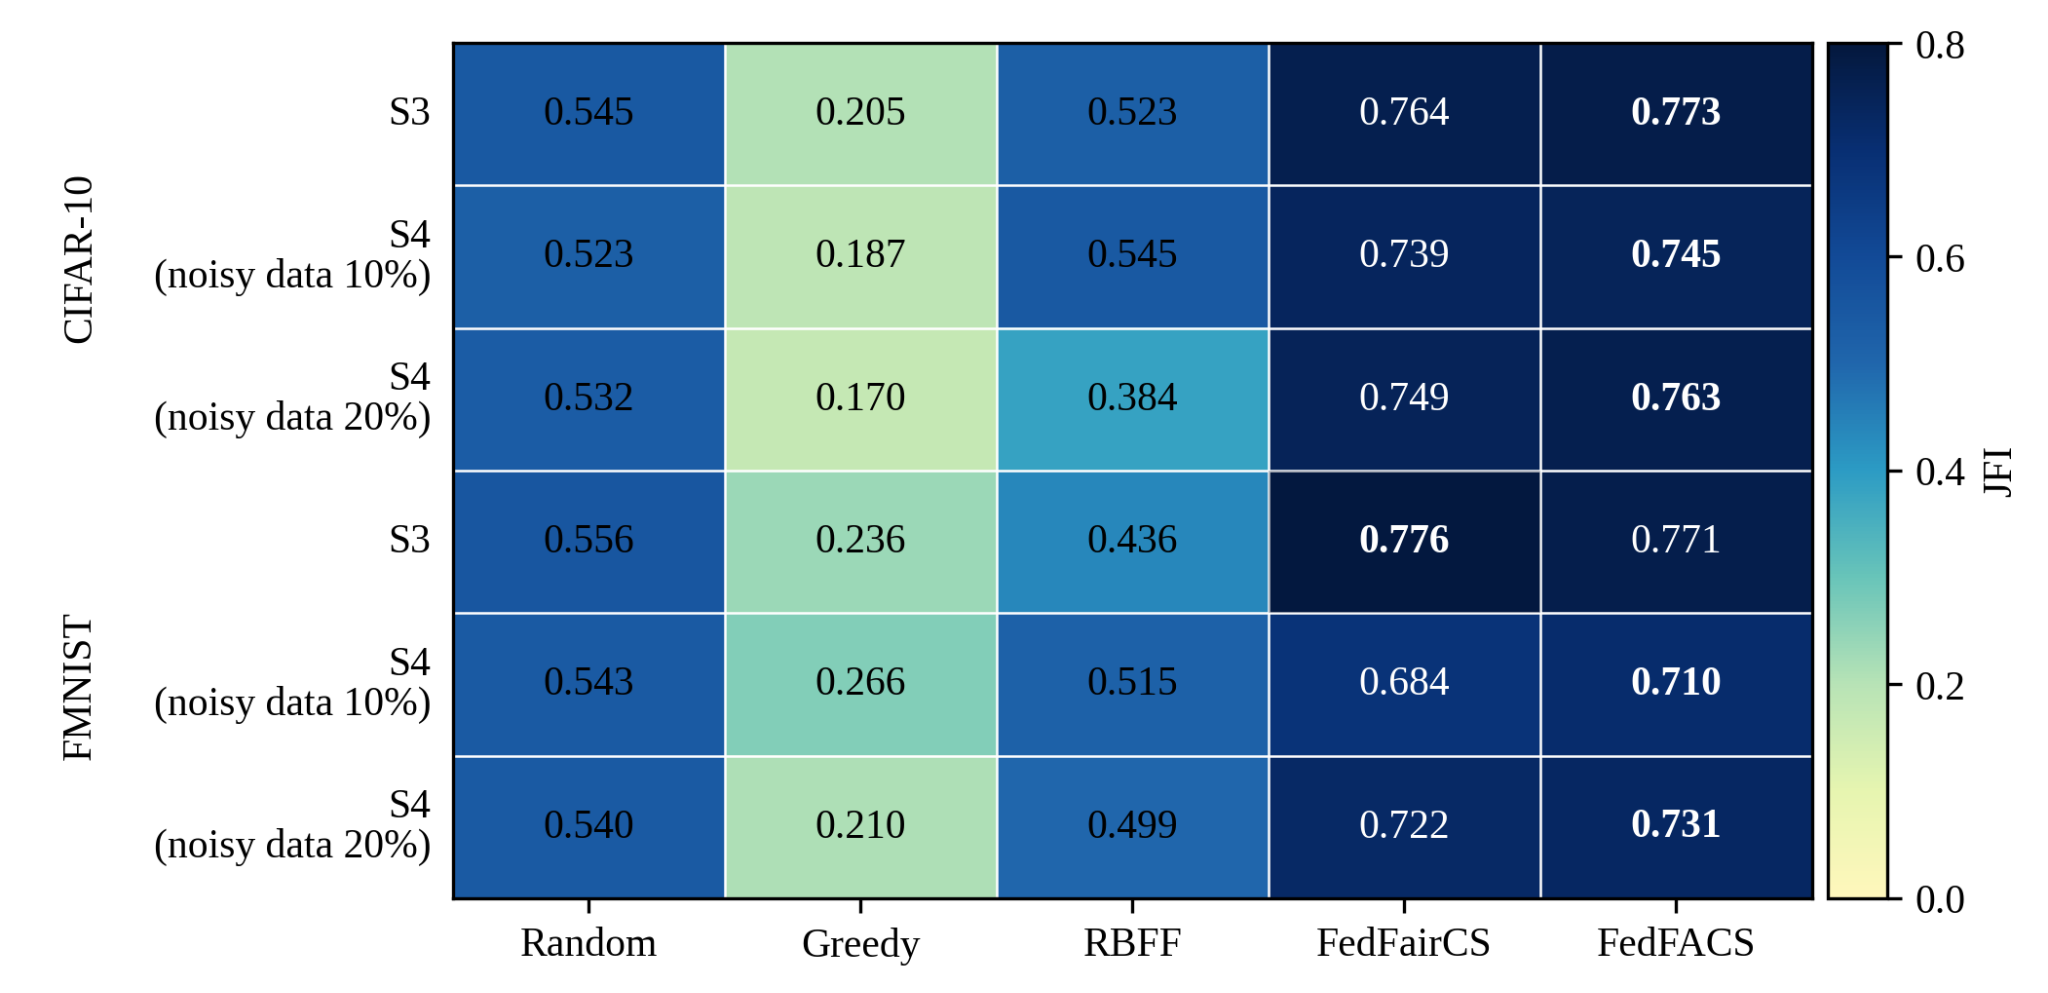
\includegraphics[width=\textwidth]{figs/fig10.png}\caption{Jain fairness index under Scenarios~3 and~4 for CIFAR-10 and FMNIST; darker cells denote higher values.}\label{fig:jfi}\end{minipage}\hfill
\begin{minipage}[t]{0.48\textwidth}\centering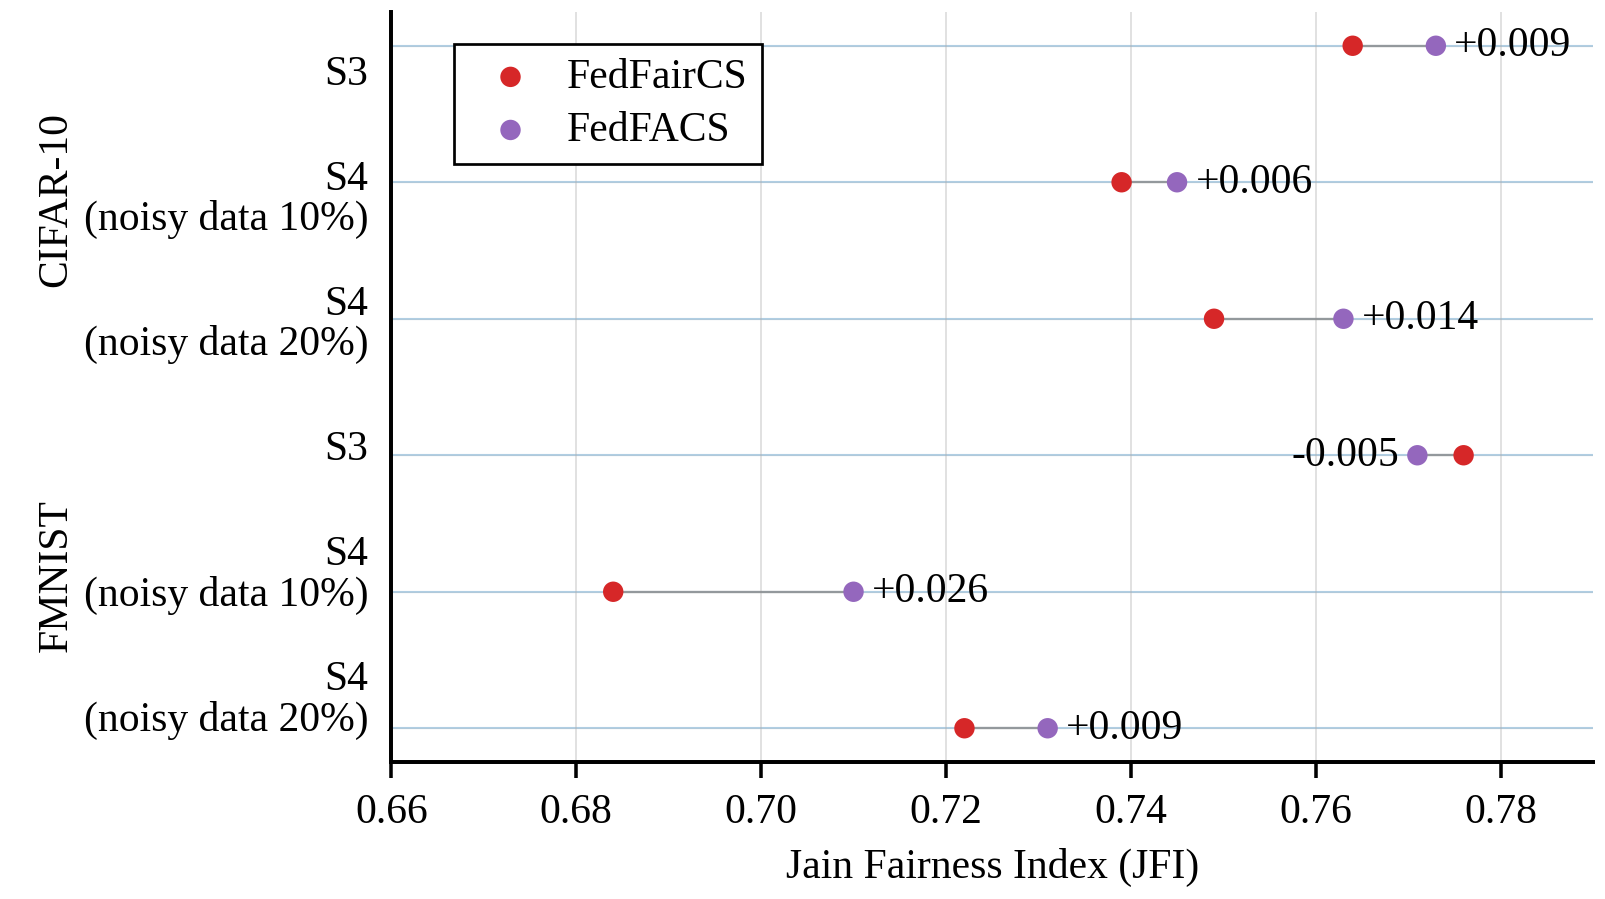
\includegraphics[width=\textwidth]{figs/fig11.png}\caption{JFI of FedFACS versus FairFedCS; annotations are signed differences.}\label{fig:jfidiff}\end{minipage}
\end{figure}

\subsubsection{Discussion}
Across the evaluated settings, the evidence supports a trade-off rather than uniform superiority. FedFACS reduced the number of rounds relative to Zhai et al.\ in every Configuration~A setting and gave modest accuracy gains in most, but it was slower than DivFL on MNIST. Relative to AHIBCS it raised accuracy and reduced cumulative uploads in all three Configuration~B datasets at the cost of more rounds on FMNIST and CIFAR-10 and lower COVID-19 recall. In Configuration C it matched or exceeded FairFedCS on JFI in five of six settings but not in all. The conditions under which the trade-off is advantageous are those in which upload volume and fairness weigh more than the extra rounds or the extra download and local-training cost borne by non-selected candidates; whether that holds for a given deployment depends on a communication and compute model that we did not measure.

%% ------------------------------------------------------------------
\section{Limitations}\label{sec:limits}
The results have the following scope and limitations.
\begin{enumerate}
\item \textbf{Correspondence between specification and results.} The results were produced before the formulation was corrected and could not be regenerated (Section~\ref{sec:scope}); the corrected specification has not been evaluated.
\item \textbf{Statistical evidence.} Every value comes from a single run, with no standard deviations or confidence intervals. Differences of one to three rounds, under one accuracy point or of 0.006 in JFI should be read as descriptive. A rigorous comparison needs at least five independently seeded runs per method with matched partitions and paired confidence intervals.
\item \textbf{Ablation.} FedFACS-A1/A2 vary cohort sizing and aggregation jointly. The individual contributions of the KL utility, fairness term, variance penalty and controller are not isolated, and the gains cannot be attributed to a specific component.
\item \textbf{Validity of the utility and the penalty.} We did not test whether $\KL_i^t$ correlates with the held-out loss change produced by incorporating a client's update, or whether the variance penalty separates corrupted from heterogeneous-but-useful updates. Sensitivity to $B$, $\mu$, $\beta$, $\lambda$, the batch size and the cohort bounds was not studied.
\item \textbf{Controller design.} The scale mismatch between $F_i^t\ge1$ and $\KL_i^t$ (Section~\ref{sec4.4}) is not corrected, and no stability, convergence or fairness guarantee is established.
\item \textbf{Communication and computation.} Only cumulative uploads were counted. All candidates download the model, train and score each round, and the corresponding downlink bytes, training steps, scoring passes and wall-clock time were not measured; the accounting of Eq.~\eqref{eq:btotal} is a definition, not a result.
\item \textbf{Fairness evidence.} JFI is quality-adjusted. Selection-frequency distributions, maximum waiting times, cumulative aggregation influence, the proportion of never-selected clients and per-client or worst-client accuracy were not recorded.
\item \textbf{Baselines.} For each baseline it is not stated whether results were reproduced in our implementation or taken from the cited publication under its own architecture and preprocessing. Oort, FedCor, q-FFL/AFL, SCAFFOLD and FedNova are discussed but not evaluated, and there is no controlled head-to-head comparison against AHIBCS, FairFedCS and Zhai et al.\ in one framework.
\item \textbf{Implementation details not recorded.} The ResNet-18 pretraining checkpoint and preprocessing, the values of $\lambda$, $\mu$ and $B$, the Configuration~B and~C cohort bounds and per-round cohort logs, the corruption process of S3 and S4, the evaluation split and accuracy endpoint (final or peak), the COVID-19 dataset version, class counts, splits and patient-level grouping, and the averaging convention of recall and F1 were not recorded.
\item \textbf{Scale and setting.} At most 100 simulated clients in a synchronous setting were used. Claims of scalability or deployment are not supported.
\item \textbf{Trust.} Client-reported scores are not verified (Section~\ref{sec4.10}); robustness to adversarial or Byzantine clients is unexplored.
\item \textbf{Reproducibility.} The code and dataset partitions behind the reported numbers are not available. A future package should contain configuration files, partition identifiers, seeds, per-round scores, cohort selections, aggregation weights and metric outputs.
\end{enumerate}

%% ------------------------------------------------------------------
\section{Conclusion}\label{sec7}
We presented FedFACS, a client selection framework that ranks clients by a fitness score combining a KL-divergence disagreement term, an idle-round fairness term and a batch-variance penalty, adapts the cohort size and utility--fairness mixing from validation-loss feedback, and aggregates selected updates with normalised nonnegative stability weights. On MNIST, FMNIST, CIFAR-10 and COVID-19 Radiography, single-run experiments show fewer rounds than Zhai et al.\ in all Configuration~A settings, higher accuracy and fewer cumulative uploads than AHIBCS in Configuration~B at the cost of more rounds on two of three datasets and lower COVID-19 recall, and a higher Jain index than FairFedCS in five of six noisy-data settings. The results describe trade-offs among accuracy, convergence rounds, uploads and quality-adjusted participation, not simultaneous superiority. They were obtained with an implementation that preceded the corrected formulation and are single-run, so they should be regarded as preliminary evidence. Future work should re-evaluate the corrected specification over multiple seeds with component-isolated ablations, measure total communication and computation, report client-level fairness, test sensitivity and scalability, and address Byzantine and data-poisoning clients.

%% ------------------------------------------------------------------
\section*{Declarations}
\begin{itemize}
\item \textbf{Funding:} \todo{authors to complete}
\item \textbf{Conflict of interest/Competing interests:} \todo{authors to complete}
\item \textbf{Ethics approval and consent to participate:} Not applicable. The study uses only publicly available benchmark datasets.
\item \textbf{Consent for publication:} Not applicable.
\item \textbf{Data availability:} MNIST, Fashion-MNIST, CIFAR-10 and the COVID-19 Radiography database are publicly available (references \citealp{lecun2010,xiao2017,krizhevsky2009,rahman2020}). The exact client partitions used in the experiments are not available.
\item \textbf{Code availability:} The implementation used to produce the reported results is not available. \todo{authors to confirm or update}
\item \textbf{Author contribution:} \todo{authors to complete}
\end{itemize}

\bibliography{sn-bibliography}

\end{document}
